% This must be in the first 5 lines to tell arXiv to use pdfLaTeX, which is strongly recommended.
\pdfoutput=1
% In particular, the hyperref package requires pdfLaTeX in order to break URLs across lines.

\documentclass[11pt]{article}

% Change "review" to "final" to generate the final (sometimes called camera-ready) version.
% Change to "preprint" to generate a non-anonymous version with page numbers.
\usepackage[final]{acl}

% Standard package includes
\usepackage{times}
\usepackage{latexsym}

% For proper rendering and hyphenation of words containing Latin characters (including in bib files)
\usepackage[T1]{fontenc}
% For Vietnamese characters
% \usepackage[T5]{fontenc}
% See https://www.latex-project.org/help/documentation/encguide.pdf for other character sets

% This assumes your files are encoded as UTF8
\usepackage[utf8]{inputenc}

% This is not strictly necessary, and may be commented out,
% but it will improve the layout of the manuscript,
% and will typically save some space.
\usepackage{microtype}

% This is also not strictly necessary, and may be commented out.
% However, it will improve the aesthetics of text in
% the typewriter font.
\usepackage{inconsolata}

%Including images in your LaTeX document requires adding
%additional package(s)
\usepackage{graphicx}

% If the title and author information does not fit in the area allocated, uncomment the following
%
%\setlength\titlebox{<dim>}
%
% and set <dim> to something 5cm or larger.

%%%%%%%%%%%%%%%%%%%%%%%%%%%%%%%%%%%%%%%%%%%%%%%%%%%%%%%%%%%%%%%%%%%%%%%%%%%%%%%%%%%%%%

% \usepackage[hidelinks]{hyperref}       % hyperlinks
\usepackage{booktabs}       % professional-quality tables
\usepackage{amsfonts}       % blackboard math symbols
\usepackage{nicefrac}       % compact symbols for 1/2, etc.
\usepackage{microtype}      % microtypography
\usepackage{xcolor}         % colors
\usepackage{multirow}
\usepackage{xspace}
\usepackage{soul}

\usepackage{longtable}
\usepackage{ulem}
\usepackage{multirow}
% \usepackage{lineno}
\usepackage{siunitx}
\usepackage{float}
\usepackage{array}
\usepackage{amsmath}
\usepackage{subcaption}
\usepackage{enumitem}
\usepackage{xcolor}
\usepackage{xspace}
\usepackage{booktabs}
\usepackage{tabularx}
\usepackage[utf8]{inputenc}
\usepackage{geometry}
\usepackage{tcolorbox}
\usepackage{lipsum}
\usepackage{makecell}
% \linenumbers
\usepackage{enumitem}
\usepackage{dcolumn}
\newcolumntype{d}[1]{D{.}{.}{#1}}

%%%%%%%%%%%%%%%%%%%%%%%%%%%%%%%%%%%%%%%%%%%%%%%%%%%%%%%%%%%%%%%%%%%%%%%%%%%%%%%%%%%%%%
% Add all custom commands here

\newcommand*\samethanks[1][\value{footnote}]{\footnotemark[#1]}
 \newcommand{\kc}[1]{\textcolor{red}{Kartik: #1}}
%\newcommand{\kc}[1]{}
\newcommand{\dieuwke}[1]{\textcolor{red!50!blue!80}{DH: #1}}
% \newcommand{\dieuwke}[1]{}

% Custom font for evaluation and judge model names
\definecolor{darkgreen}{RGB}{0,100,0}
\definecolor{red}{RGB}{255,0,0}
% \newcommand{\eval}[1]{{\textcolor{darkgreen}{#1}}}
\newcommand{\eval}[1]{{\fontfamily{phv}\selectfont #1}}
\newcommand{\judge}[1]{\texttt{\textcolor{black}{#1}}}

\newcommand{\njudges}{13\xspace}
\newcommand{\njudgesword}{thirteen\xspace}
\newcommand{\nexamtakers}{9\xspace}
\newcommand{\nexamtakersword}{nine\xspace}

\newcommand{\evaluatormodel}{exam-taker model\xspace}
\newcommand{\evaluatormodels}{exam-taker models\xspace}
\newcommand{\Evaluatormodel}{Exam-taker model\xspace}
\newcommand{\Evaluatormodels}{Exam-taker models\xspace}

\newcommand{\judgemodel}{judge model\xspace}
\newcommand{\judgemodels}{judge models\xspace}
\newcommand{\Judgemodel}{Judge model\xspace}
\newcommand{\JudgeModel}{Judge Model\xspace}
\newcommand{\Judgemodels}{Judge models\xspace}
\newcommand{\JudgeModels}{Judge Models\xspace}


\newcommand{\scottspi}{Scott's $\mathbf{\pi}$\xspace}
\newcommand{\cohenskappa}{$\kappa$ \textcolor{red}{TO CHANGE!}}
\newcommand{\gpt}{GPT-4\;Turbo\xspace}

\newcommand{\specialcell}[2][c]{\footnotesize\begin{tabular}[#1]{@{}l@{}}#2\end{tabular}}


\tcbset{
  outerbox/.style={
    colback=white,
    colframe=black,
    fonttitle=\bfseries,
    boxrule=0.25mm,
    sharp corners,
    rounded corners,
  }
}

% Define the custom tcolorbox macro
\def\mytcolorbox#1#2#3{
  \begin{tcolorbox}[outerbox, title={\textit{#1}}]
  \texttt{#2} \\
  \\
  \texttt{#3}
  \end{tcolorbox}
}


%%%%%%%%%%%%%%%%%%%%%%%%%%%%%%%%%%%%%%%%%%%%%%%%%%%%%%
% Cleverref
\usepackage[noabbrev,capitalize,nameinlink]{cleveref}
\crefname{section}{Section}{Sections}%{\S}{\S\S}
% \crefname{table}{Tab.}{}
\crefname{table}{Table}{}
% \crefname{figure}{Fig.}{}
\crefname{figure}{Figure}{}
\crefname{section}{\S}{\S\S}
\Crefname{section}{\S}{\S\S}
\crefname{appendix}{Appendix}{Appendices}
\Crefname{Appendix}{Appendix}{}

\title{Judging the Judges: Evaluating Alignment and Vulnerabilities in LLMs-as-Judges}

\author{Aman Singh Thakur\thanks{Equal Contribution} \and Kartik Choudhary\samethanks \and Venkat Srinik Ramayapally\samethanks \\
  University of Massachusetts Amherst \\
  \texttt{\{amansinghtha, kartikchoudh, vramayapally\}@umass.edu} \\\AND
  Sankaran Vaidyanathan \\
  University of Massachusetts Amherst \\
  \texttt{sankaranv@cs.umass.edu} \\\And  
  Dieuwke Hupkes \\
  Meta \\
  \texttt{dieuwkehupkes@meta.com}
  }

%%%%%%%%%%%%%%%%%%%%%%%%%%%%%%%%%%%%%%%%%%%%%%%%%%%%%%

\begin{document}
\maketitle

\begin{abstract}

The \textit{LLM-as-a-judge} paradigm offers a potential solution to scalability issues in human evaluation of large language models (LLMs), but there are still many open questions about its strengths, weaknesses, and potential biases. This study investigates \njudgesword models, ranging in size and family, as `\textit{\judgemodels}' evaluating answers from \nexamtakersword base and instruction-tuned `\textit{\evaluatormodels}'. We find that only the best (and largest) models show reasonable alignment with humans, though they still differ with up to 5 points from human-assigned scores. Our research highlights the need for alignment metrics beyond percent agreement, as judges with high agreement can still assign vastly different scores. We also find that smaller models and the lexical metric \judge{contains} can provide a reasonable signal in ranking the \evaluatormodels. Further error analysis reveals vulnerabilities in \judgemodels, such as sensitivity to prompt complexity and a bias toward leniency. Our findings show that even the best \judgemodels differ from humans in this fairly sterile setup, indicating that caution is warranted when applying \judgemodels in more complex scenarios.

% Offering a promising solution to the scalability challenges associated with human evaluation, the \textit{LLM-as-a-judge} paradigm is rapidly gaining traction as an approach to evaluating large language models (LLMs).
% However, there are still many open questions about the strengths and weaknesses of this paradigm, and what potential biases it may hold.
% In this paper, we present a comprehensive study of the performance of various LLMs acting as judges
% % \footnote{Source code is available at \url{https://github.com/UMass-Meta-LLM-Eval/llm_eval}}
% % We leverage TriviaQA as a benchmark for assessing objective knowledge reasoning of LLMs and evaluate them alongside human annotations which we found to have a high inter-annotator agreement. 
% Investigating \njudgesword \textit{\judgemodels} of different model sizes and families, judging answers of \nexamtakersword different `\textit{\evaluatormodels}' -- both base and instruction-tuned -- we find that only the best (and largest) models achieve reasonable alignment with humans.
% However, they are still quite far behind inter-human agreement and their assigned scores may still differ with up to 5 points from human-assigned scores.
% In terms of their ranking of the \nexamtakersword \evaluatormodels, instead, also smaller models and even the lexical metric \judge{contains} may provide a reasonable signal.
% Through error analysis and other studies, we identify vulnerabilities in \judgemodels, such as their sensitivity to prompt complexity and length, and a tendency toward leniency.
% The fact that even the best judges differ from humans in this comparatively simple setup suggest that caution may be wise when using judges in more complex setups.
% Lastly, our research rediscovers the importance of using alignment metrics beyond simple percent alignment, showing that judges with high percent agreement can still assign vastly different scores.

% We find that \judge{Llama-3\;70B}, \judge{Llama-3.1\;70B} and \judge{GPT-4\;Turbo} have an excellent alignment with humans, but in terms of \textit{ranking} exam taker models, they are not better than some smaller models and even the lexical matching method \judge{Contains}, which have up to 24 points lower human alignment. 
% Furthermore, the basic lexical \judge{Contains} match and the fine-tuned \judge{JudgeLM-7B} maintain the \textit{ranking} of \evaluatormodels better than larger and highly aligned models like \judge{\gpt} and \judge{Llama-3 70B}, despite having kappa scores up to 34 points lower than human alignment. 
% We find that both Llama-3-70B and GPT-4 have excellent alignment with humans, but in terms of \textit{ranking} \evaluatormodels, they are outperformed by both JudgeLM-7B and the lexical matching method \judge{contains}.
% Finally, our error analysis highlights vulnerabilities inherent in judgemodels.

% Through error analysis and various other studies, including the effects of instruction length and leniency bias, we hope to provide useful lessons for using LLMs as judges in the future.

% We discover that both Llama-3 and GPT-4 have very high alignment with humans, does this alignment 
% Our research uncovers substantial misalignment between \judgemodels and human annotations.  
% We demonstrate that although models such as Llama 3 and GPT-4 exhibit high alignment, this alignment does not correlate with comparable evaluation scores. 
% Furthermore, we observe that basic lexical matching techniques more precisely replicate the rankings of exam-taker models assigned by humans compared to all \judgemodels.
% Finally, our error analysis highlights vulnerabilities inherent in \judgemodels, particularly in instruction-tuned models.Further examination of their prompt sensitivities and biases reveals that they are often lenient and susceptible to manipulation.
\end{abstract}

\section {Introduction} \label{sec:intro}

\begin{figure*}[t]
    \centering
    \begin{subfigure}[b]{0.55\textwidth}
        \centering
        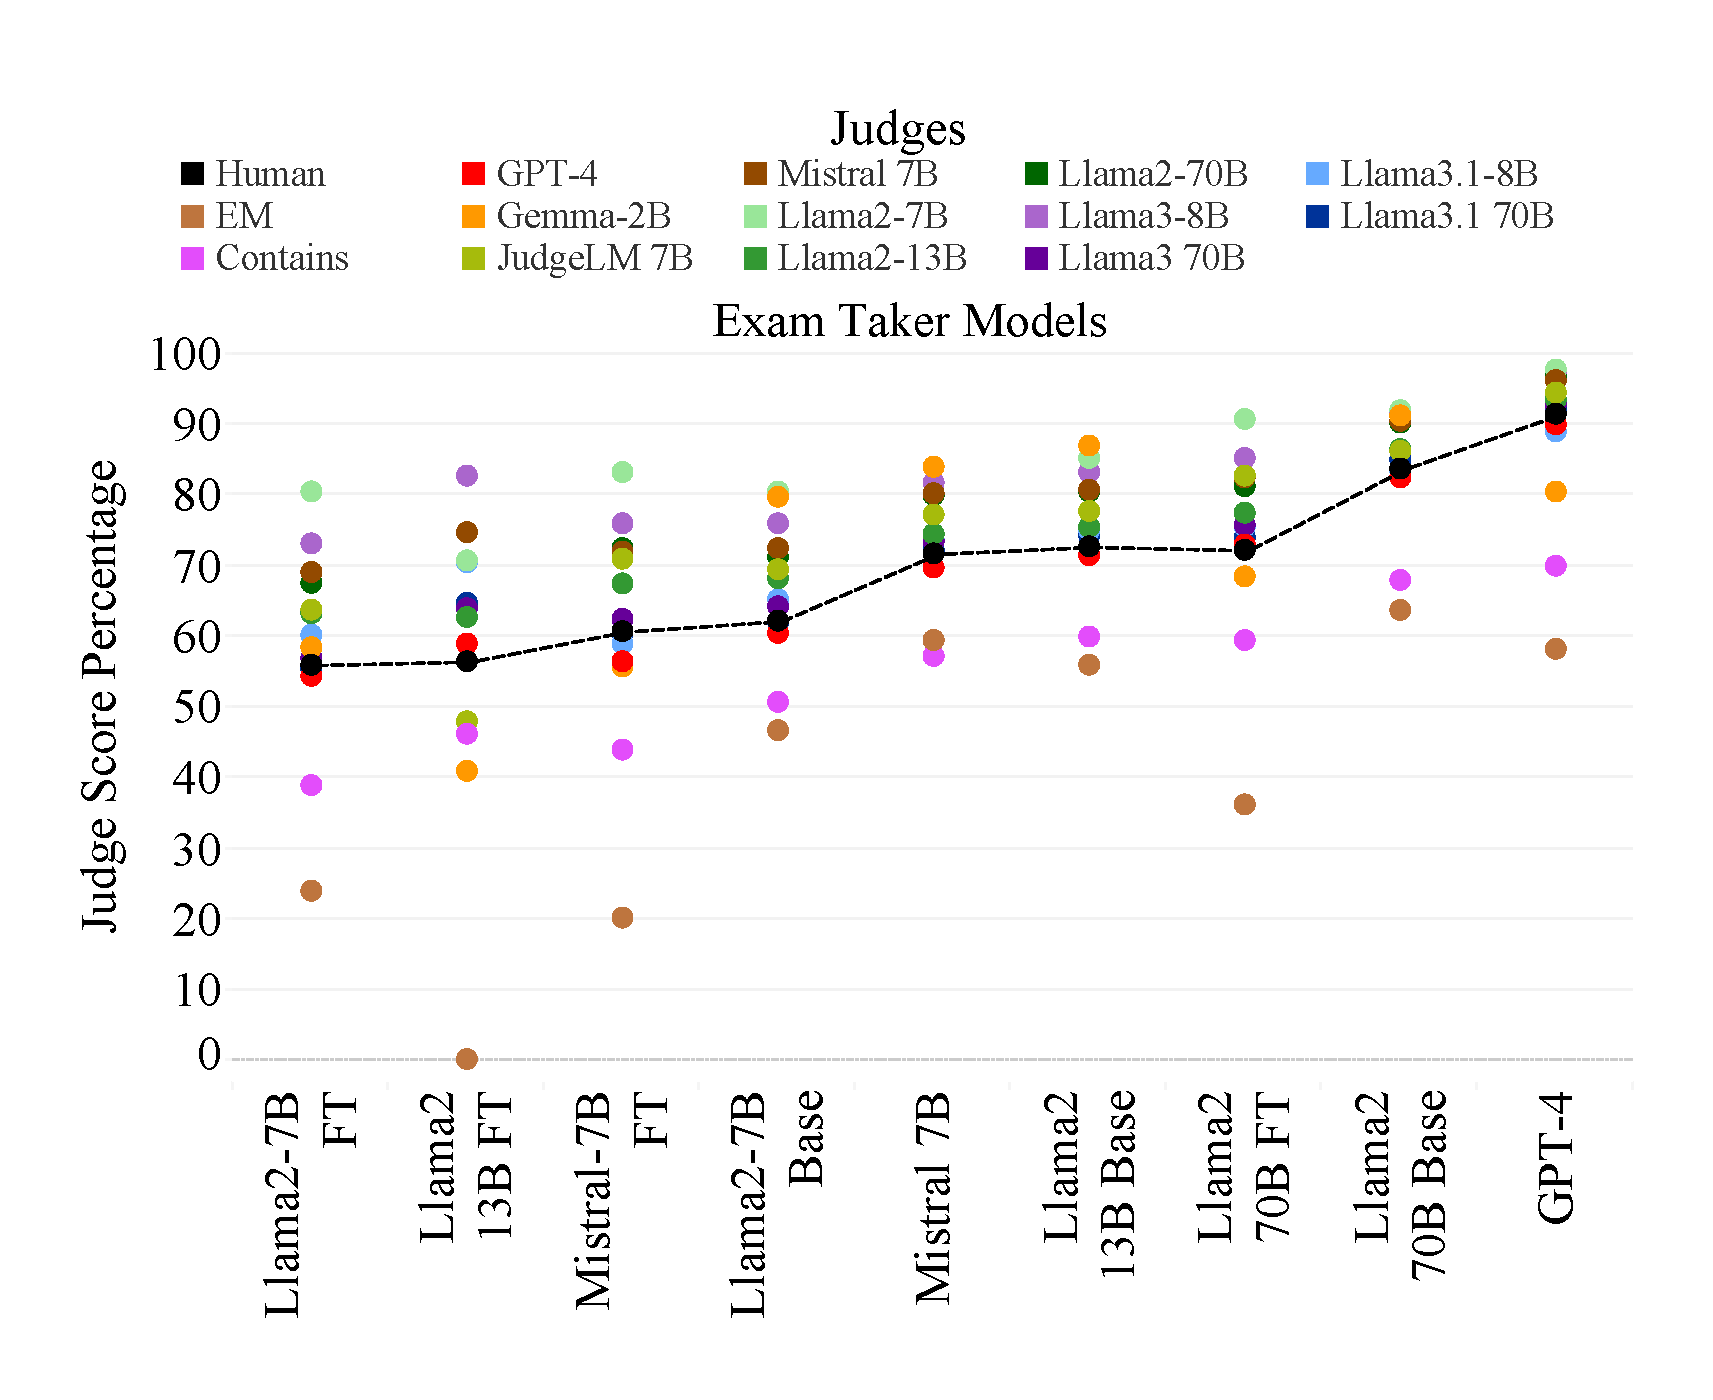
\includegraphics[width=\linewidth]{figures/Scores_HG_V3.pdf}
        \vspace{-6mm}
        \caption{}
        \vspace{-2mm}
        \label{fig:llmalignment_a}
    \end{subfigure}
    \hfill
    \begin{subfigure}[b]{0.44\textwidth}
        \centering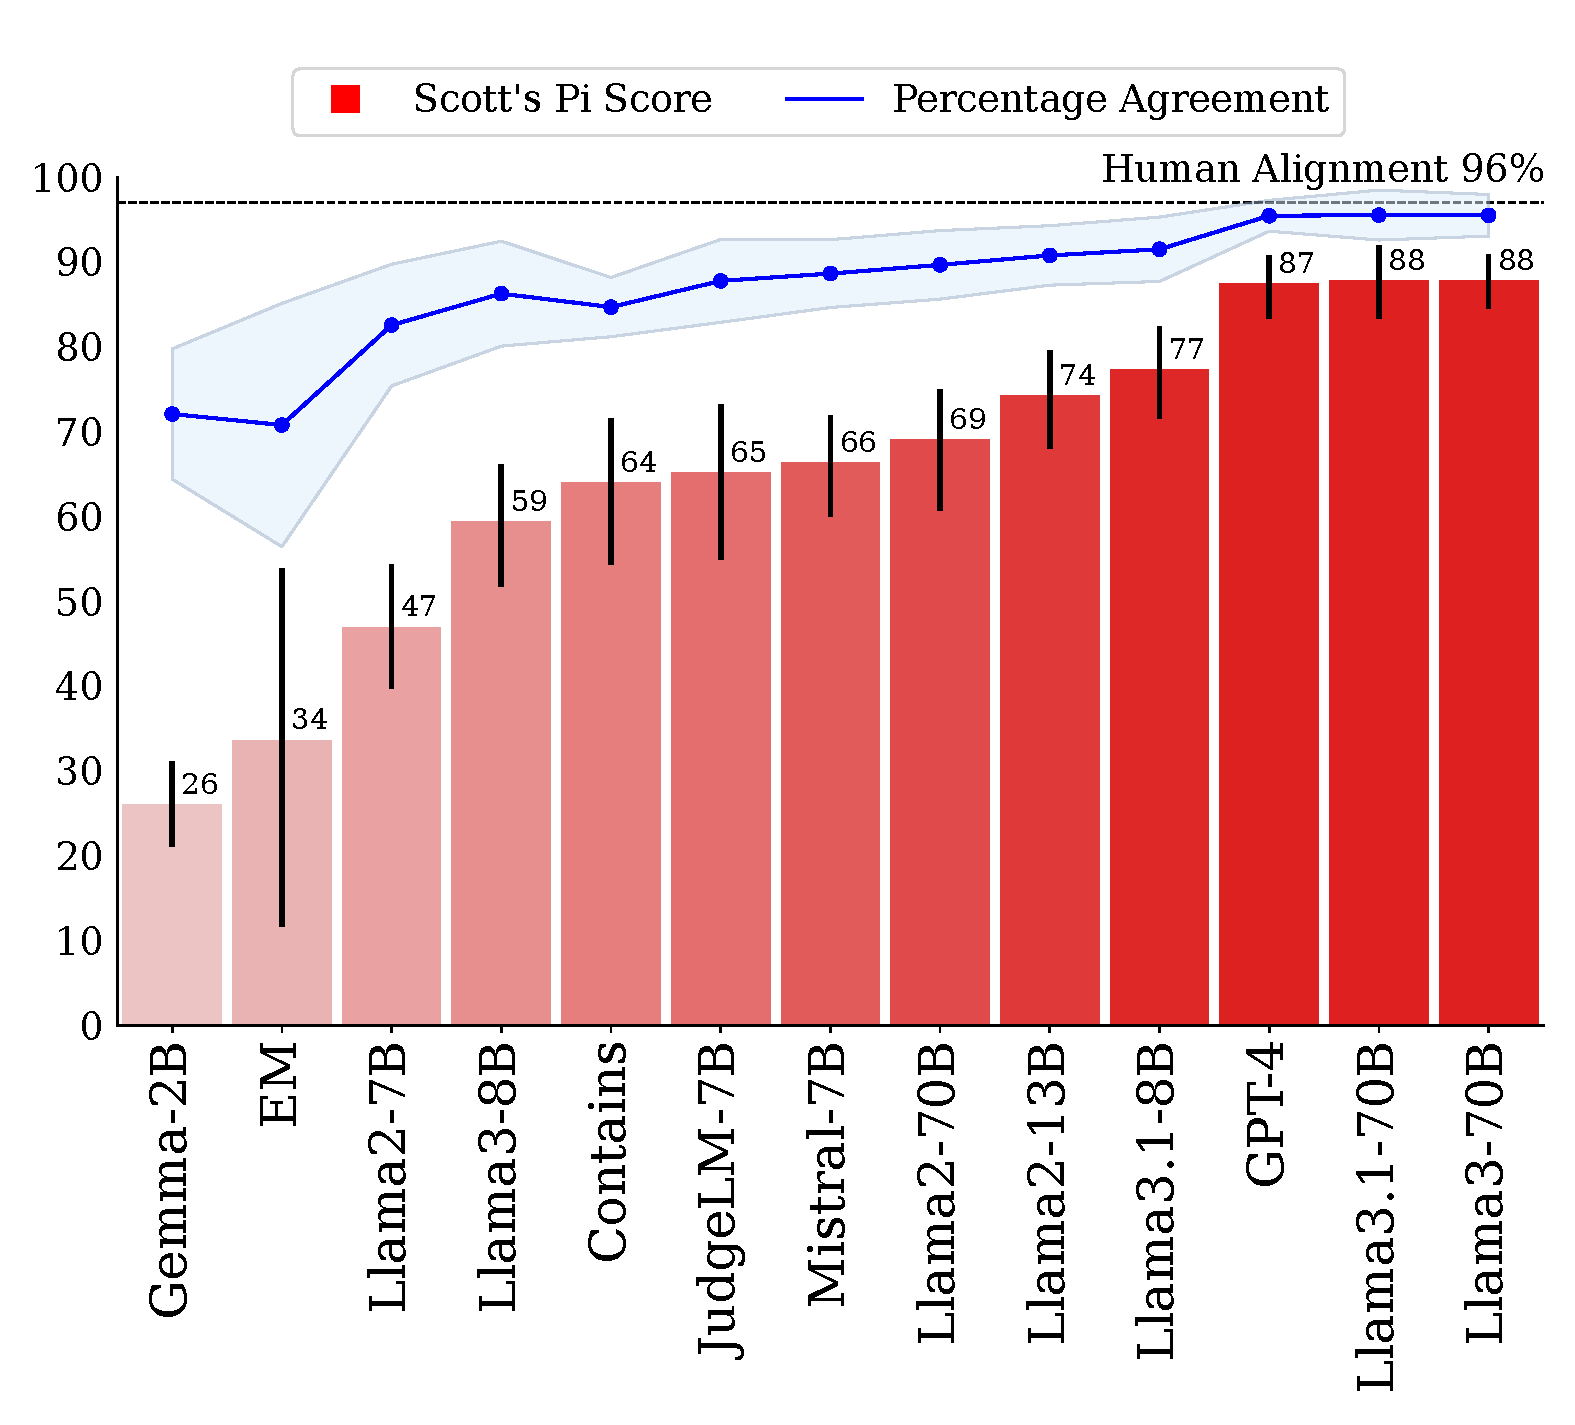
\includegraphics[width=\linewidth, height=6.5cm]{figures/LLMAlignment_HG_V1.pdf}
        \vspace{-6mm}
        \caption{}
        \vspace{-2mm}
        \label{fig:llmalignment_b}
    \end{subfigure}
    \caption{\textbf{Average scores assigned by judge models and alignment with human judges.} (a) Scores assigned to all \evaluatormodels by the various \judgemodels. 
    (b) Average percent agreement (blue line) and Scott's $\pi$ scores (red bars) of \judgemodels with human judges (black line).
    Error bars annotate standard deviation across \evaluatormodels. 
    \judge{Llama3 70B}, \judge{Llama3.1 70B} and \judge{\gpt} have Scott's $\pi$ coefficient that are indicative of excellent alignment, but are still well below the human alignment score. % of 96\%.
    }
    \label{fig:llmalignment}
\end{figure*}

Over the last few years, large language models (LLMs) have demonstrated remarkable capabilities across various domains \citep[i.a.]{radford2019language, brown2020language, achiam2023gpt, meta2024llama3}.
% world knowledge \citep{petroni2019language, razeghi2022impact} and the ability to learn specialized tasks from a few examples \citep{brown2020language}. 
% They have been employed in various tasks including generating free-form responses \citep{}, condensing extensive textual data \citep{pu2023summarization}, conducting search \citep{}, categorizing or grouping documents \citep{}, and facilitating question-answering systems \citep{vectara_llm_use_cases}. 
% 
As more and more new LLMs with different architectures and training methods continue to be released and their capabilities expand, accurately evaluating their performance and limitations becomes increasingly challenging \citep{zheng2024judging,ohmer2024form,benchekroun2023worldsense,madaan2024quantifying,li2023generative}.
% The empirical evaluation of LLMs is particularly difficult due to the diversity of their outputs and the variety of tasks they are used for \citep{li2023generative}. 


LLM evaluation methods generally fall into one of two broad categories. Benchmarks such as MMLU \citep{mmlu}, TruthfulQA \citep{lin2021truthfulqa}, and GSM8K \citep{cobbe2021training} assess specific capabilities, while leaderboards such as Chatbot Arena \citep{chiang2024chatbot} and Open LLM Leaderboard \citep{open-llm-leaderboard} rank models based on human or automated pairwise comparisons. Both approaches face challenges in evaluating free-form text responses, as assessment can be as difficult as generation itself \citep[see e.g.][]{chang2023survey, bavaresco2024llmsinsteadhumanjudges}.

% To evaluate LLMs, various methods have been proposed, typically falling into one of two broad categories. 
% First, benchmarks such as MMLU \citep{mmlu}, TruthfulQA \citep{lin2021truthfulqa}, or GSM8K \citep{cobbe2021training} are used to evaluate specific capabilities of LLMs in an automated manner. 
% Additionally, leaderboards like Chatbot Arena \citep{chiang2024chatbot} and Open LLM Leaderboard \citep{open-llm-leaderboard} assign ranks to models considering pair-wise rankings of LLM outputs, done by humans or, in some cases, automated evaluation methods.
% Since both strategies involve evaluating free-form text responses generated by the LLMs, even in the first case, evaluating the responses is often just as challenging as generating them \citep[see e.g.][]{chang2023survey, bavaresco2024llmsinsteadhumanjudges}. 

One approach to evaluating LLMs is using MCQ benchmarks like MMLU, which compare answer log-probabilities instead of assessing generated responses directly. However, this approach limits the range of measurable abilities and differs from how LLMs are used in practice. Lexical methods, such as exact match (EM) or n-gram overlap, are practical and cost-effective but prone to false negatives and often miss subtle semantic differences. These challenges are amplified for instruction-tuned chat models, which tend to produce more verbose responses \citep{saito2023verbosity, renze2024benefits}.

% One proposed solution to this problem is to use multiple-choice question (MCQ) benchmarks such as MMLU, and compare the log-probabilities of the potential answers rather than evaluating the generated answer directly. 
% However, the MCQ paradigm limits the range of abilities that can be evaluated, and the setup increasingly diverges from how LLMs are used in practice.
% Alternatively, the use of lexical matching methods such as exact match (EM) or n-gram overlap to evaluate the responses are practical and cost-efficient approaches, but are susceptible to false negatives and often fail to adequately distinguish between responses with subtle differences that change their semantic meaning.
% This issue is exacerbated when evaluating instruction-tuned ``chat'' models that are fine-tuned to carry out conversations with humans in natural language, since their responses tend to be more verbose \citep{saito2023verbosity, renze2024benefits}. 
% 
For these reasons, human evaluation remains the gold standard for evaluating LLM responses. %, especially since many benchmarks aim to assess how useful the LLMs are to humans. 

\begin{table*}
    \centering
    \renewcommand{\arraystretch}{1.1} % Increase row height
    \begin{tabular}{|>{\centering\arraybackslash}m{4.5cm}|>{\arraybackslash}m{9cm}|}
        \hline
        \textbf{\Evaluatormodels (base \& instruction-tuned)} & \eval{Llama-2 (7B, 13B, 70B)}, \eval{Mistral 7B}, \eval{\gpt} \\
        \hline
        \textbf{\Judgemodels (instruction-tuned)} & \judge{Llama-2 (7B, 13B, 70B)}, \judge{Llama-3 (8B, 70B)}, \judge{Llama-3.1 (8B, 70B)}, \judge{Gemma 2B}, \judge{Mistral 7B}, \judge{JudgeLM 7B}, \judge{\gpt} \\
        \hline
        \textbf{\Judgemodels (lexical)} & \judge{Exact Match (EM), Contains} \\
        \hline
    \end{tabular}
     \caption{\textbf{\Evaluatormodels and \judgemodels} We consider a wide variety of \evaluatormodels and \judgemodels; to get an in-depth overview of their abilities, we consider \evaluatormodels of various sizes \& types.}
    \label{tab:evaluation}
\end{table*}

Human evaluation is, however, expensive and often impractical, leading to the growing use of LLMs as \judgemodels \citep{lin2021truthfulqa,islam2023financebench,chiang2023can,liusie2024llm}. While promising alignment with humans has been noted \citep{sottana2023evaluation,zheng2024judging}, questions about this approach remain. This work examines LLMs as judges, contrasting them with humans and automated methods. Unlike prior studies, we focus on scenarios with high human alignment to separate task ambiguity from \judgemodel limitations. Using TriviaQA \citep{joshi2017triviaqa}, we evaluate how \textit{\judgemodels} of varying architectures and sizes assess \textit{\evaluatormodels}.

% However, human evaluation is expensive, time-consuming, and often impractical in many use cases. 
% As a result, it has increasingly become common practice to evaluate LLM responses using another LLM as a \judgemodel \citep{lin2021truthfulqa,islam2023financebench,chiang2023can,liusie2024llm}.
% While there are promises of alignment between LLM judges and humans \citep{sottana2023evaluation,zheng2024judging}, there are also many open questions about the strengths and weaknesses of the paradigm.
% 
In this work, we study the properties of LLMs as judges, comparing them with humans and automated evaluation methods.
Contrary to prior work, we focus on a clean scenario in which human alignment is very high, 
allowing us to distinguish ambiguity and subjectivity in the task itself from potential issues with the \judgemodels.
Using the knowledge benchmark TriviaQA \citep{joshi2017triviaqa} as our playground, we investigate how \njudgesword different \textit{\judgemodels} with varying architectures and sizes judge \nexamtakersword different \textit{\evaluatormodels}.
% Our main findings are:\begin{itemize}[wide, labelwidth=2pt, labelindent=2pt]\setlength\itemsep{1em}
    Our main findings are:
    % \vspace{-1mm}
% \begin{itemize}[wide, labelwidth=2pt, labelindent=2pt,topsep=-4pt, itemsep=-2pt]%\setlength\itemsep{1em}
\begin{itemize}[leftmargin=4pt, topsep=1pt, itemsep=0.1em] %\setlength\itemsep{0.1em}
    \item \textbf{Even in clean setups, only the best models have high alignment scores}. Among the \njudgesword \judgemodels, only \judge{\gpt}, \judge{Llama-3.1;70B}, and \judge{Llama-3;70B} achieved strong alignment with humans. However, even these fall short of the human alignment coefficient (\cref{fig:llmalignment}). %\vspace{-1mm}
% \item While previous work commonly used percent agreement, \textbf{Cohen's kappa distinguishes judges much better}, since in some cases, high percent agreement can still give very divergent scores (\cref{fig:cohenskappa}).
\\
\item \textbf{\scottspi distinguishes judges better than percent alignment}. In terms of percent alignment, judges are rarely discriminable, while \scottspi provides a more informative signal. In some cases, high percent agreement can still give scores that differ 10-20 points from the human-assigned scores (\cref{fig:alignment_vs_delta}). %\vspace{-0.5mm}

\item \textbf{Also \scottspi is not all telling} While \judge{\gpt} and \judge{Llama-3} achieve excellent alignment scores, they can differ by up to 5 points from human scores. Moreover, in discriminating between \evaluatormodels, their performance is comparable to cheaper alternatives like \judge{Mistral 7B} and \judge{contains}, which have lower alignment scores but more consistent biases (\cref{fig:ranking_posneg}).

% \item \textbf{Also \scottspi is not all telling}. While \judge{\gpt} and \judge{Llama-3} both have alignment scores that are considered excellent, their scores still differ up to 5 points from human-assigned scores. Furthermore, when it comes to \textit{discriminating} different \evaluatormodels, their results are comparable to alternative cheaper approaches such as \judge{Mistral\;7B} and \judge{contains}, which have much lower alignment scores but more consistent biases (\cref{fig:ranking_posneg}).

\end{itemize}

Through detailed analysis (\cref{sec:analysis}), we gain insights into judge performance. Improved alignment appear to be driven from higher recall rates and fewer false negatives. However, \judgemodels struggle with under-specified answers and exhibit leniency, reducing evaluation consistency. They are also sensitive to prompt length and quality. Surprisingly, even when asked to evaluate a verbatim match with a reference, \judgemodels sometimes fail.

Overall, our work highlights the strengths of the LLM-as-a-judge paradigm, while cautioning against overreliance on alignment metrics, even when they are high. Through error analysis, we identify common failure cases, contributing to a deeper understanding of this emerging evaluation paradigm. With this work, our objective is to improve understanding of the emerging mainstream paradigm for evaluating LLM.

% Through detailed analysis (\cref{sec:analysis}), we uncover additional insights into judge performance. 
% Improved alignment appears to be driven by improved recall rates and reduced false negatives. 
% However, \judgemodels struggle with under-specified answers and tend to be lenient, affecting their evaluation consistency. 
% They are also sensitive to the length and quality of prompts.
% And, surprisingly, even when the \judgemodels are asked to evaluate an answer matching verbatim with a reference answer, many \judgemodels still sometimes fail to evaluate it correctly.

% Overall, our work showcases the strengths of the LLM-as-a-judge paradigm while also highlighting the need for caution against overreliance on alignment metrics, even in cases where they are high.

% Through error analysis, we also highlight several common failure cases that require attention.
% With this, we aim to contribute to a better general understanding of what is now becoming a mainstream paradigm for evaluating LLMs.


\section {Related work}\label{sec:relatedwork}

Various recent studies have used or considered using LLMs as judges for tasks such as evaluating story generation \citep{chiang2023can}, retrieval-augmented generation \citep{es2023ragas},  visual QA \citep{maas2024improving}, code comprehension \citep{yuan2023evaluating}, multilingual evaluation \citep{hada2023large} and more general open-ended tasks \citep{zheng2024judging}.
\citet{Zhang2024LLMEval} and \citet{sottana2023evaluation} propose ways to standardise LLM evaluations and the role that \judgemodels might play in such solutions.
Several studies have demonstrated that state-of-the-art LLMs such as \gpt exhibit high alignment with human judgments \citep{sottana2023evaluation,zheng2024judging}, though others also illustrate that the paradigm is not yet without faults.
\citet{zeng2023evaluating} propose a benchmark for evaluating the performance of LLMs as judges, and other approaches have been proposed to improve LLM judges such that they are aligned well with humans \citep{shankar2024validates,zhu2023judgelm}.

Despite promising results in various settings, \judgemodels still suffer from known issues of current LLMs such as hallucinations and factual errors \citep{ye2023cognitive, turpin2023language} and difficulty in following complex instructions \citep{li2023instruction, he2024can}. 
Furthermore, various studies have reported challenges such as position bias \citep{pezeshkpour2023large,zheng2023large,wang2023large}, verbosity bias \citep{saito2023verbosity} in their preferences, confusing evaluation criteria \citep{hu2024llm}, or focusing more on the style and grammar compared to factuality \citep{wu2023style}.
Recently, \citet{liusie2024llm} have shown that LLMs perform better in comparative assessment compared to absolute scoring, which can be used for reliably measuring the relative performance of models \citep{liu2024aligning} and creating classifiers for pairwise grading 
\citep{llmasclassifier}.

We build on previous work to investigate the strengths and weaknesses of LLMs as judges. Unlike previous studies, we focus on comparing LLM outputs with reference answers rather than pairwise comparisons on open-ended tasks. With high human alignment in this setting, we gain a clearer view of LLM performance. Furthermore, we extend previous research by considering more LLMs, both as judges and as evaluated models.

% We follow up on this line of work and investigate the strengths and weaknesses of LLMs as judges.
% Unlike most prior work, we do not focus on pairwise comparisons of LLM outputs on open-ended tasks, but on comparisons of LLM outputs and reference answers.
% Since human alignment is high in this setting, this provides a clean playground to study the strengths and weaknesses of LLMs in detail.
% We also extend previous work by considering more LLMs, both as judges and LLMs to be evaluated.

% The judges are evaluated not only with percent agreement, but also with \emph{Cohen's kappa coefficient} \citep{cohen1960kappa} which is commonly considered more robust, and the way they rank different models, which as we will see may sometimes paint vastly different pictures.

% However, the strengths, weaknesses and biases of this \emph{LLM-as-a-judge} paradigm have not been studied in detail.
% Prior work has demonstrated that LLMs such as \judge{GPT-4} exhibit high alignment with humans in such tasks when used as a judge \citep{sottana2023evaluation,zheng2024judging}. 
% Despite promising results in various settings, \judgemodels still suffer from the issues of current LLMs, such as hallucinations and factual errors \citep{ye2023cognitive, turpin2023language} and difficulty in following complex instructions \citep{li2023instruction, he2024can}. Moreover, use of LLMs as judges can give rise to unique challenges such as exhibiting position bias \citep{pezeshkpour2023large} and verbosity bias \citep{saito2023verbosity} in their preference, confusing the evaluation criteria \citep{hu2024llm}, or focusing more on the style and grammar of the response compared to its factuality \citep{wu2023style}.
% % However, the strengths, weaknesses and biases of this \emph{LLM-as-a-judge} paradigm have not been studied in detail.


\section{Methodology}\label{sec:methodology}

% \kc{Describe metrics and how to perform  benchmarks here so that in the next section we talk about what specific experiments we are running? Right now they are kind of mixed I think.}

To evaluate the strengths and weaknesses of the LLM-as-a-judge paradigm, we focus on a comparatively controlled setup, in which \judgemodels assess answers of \evaluatormodels on the knowledge benchmark TriviaQA \citep{joshi2017triviaqa}.
With this methodological design, it is possible to focus on the abilities of the judges in isolation, without having to address human disagreement and error at the same time.
In this section, we elaborate the main aspects of our methodology.
\setlength{\parskip}{1pt}
% To obtain a comprehensive picture, we consider several state-of-the-art models often used as judges, a model specifically trained to judge, and several smaller autoregressive models.
% In total, we consider \njudgesword \judgemodels and \nexamtakersword \evaluatormodels.
% More details about the dataset and models are provided in \cref{app:asset-details}.

% \subsection{Benchmark and evaluation metrics}\label{sec:experiments:benchmark}

\paragraph{Evaluation data}
% \subsection{Evaluation data}
%
As our testbed, we use the TriviaQA dataset \citep{joshi2017triviaqa}, consisting of 95K question-answer pairs sourced from 14 trivia and quiz league websites. 
Each question in the train and validation set is annotated with a list of short answers containing a minimal set of facts and evidence documents collected from Wikipedia and the Web.
For our experiments, we use the validation set of the \textit{unfiltered} partition of the benchmark, using the short answers as reference answers.
We use the training set for few-shot examples.

Since experiments require manual annotation of the \evaluatormodel responses, we use a random sample of $400$ questions from the dataset.
In \cref{app:downsamplingstddev}, we show with a bootstrapping test that this sample size has low variance for our main result.
Through experiments described in \cref{subsec:human_alignment}, we establish that humans have high agreement on  judgements of answers given to the questions in the benchmark.

% \subsection{\Evaluatormodels} \label{sec:experiments:evaluationmodel}

\begin{figure*}
    \centering
    \begin{subfigure}[b]{0.415\textwidth}
        \centering
        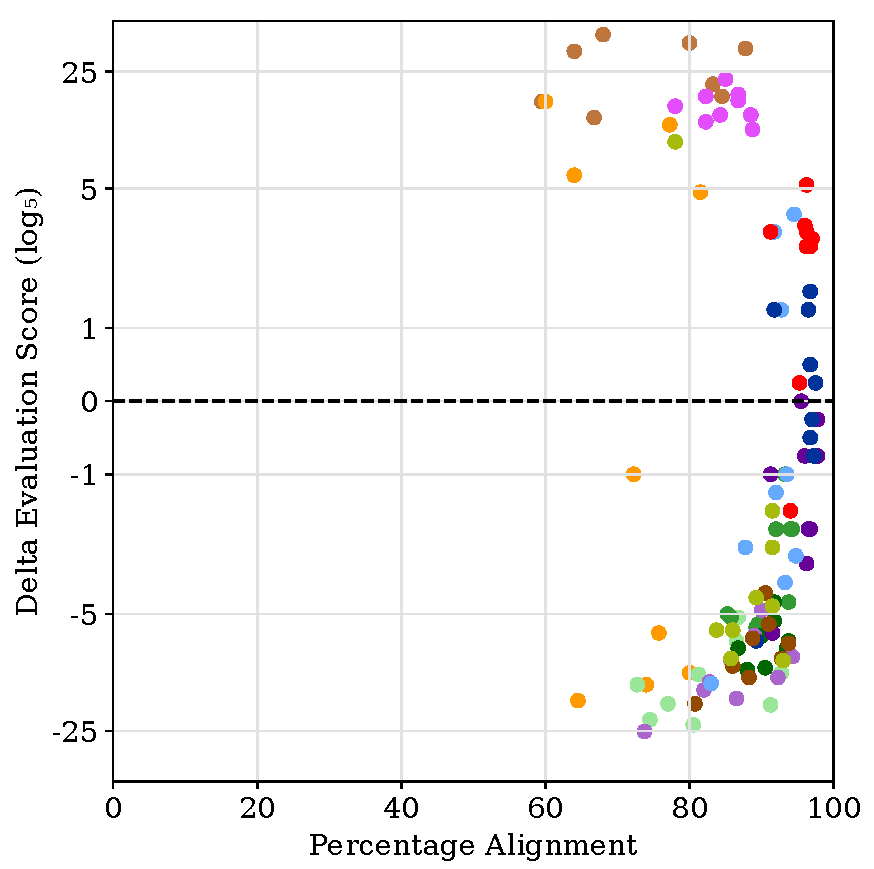
\includegraphics[width=0.9\linewidth]{figures/ScottsPiScoreVariation_aV2.pdf}
        % \vspace{-2mm}
        % \caption{}
        % \vspace{-2mm}
        % \label{fig:pct_aligned_vs_delta}
    \end{subfigure}%
    \begin{subfigure}[b]{0.565\textwidth}
        \centering
        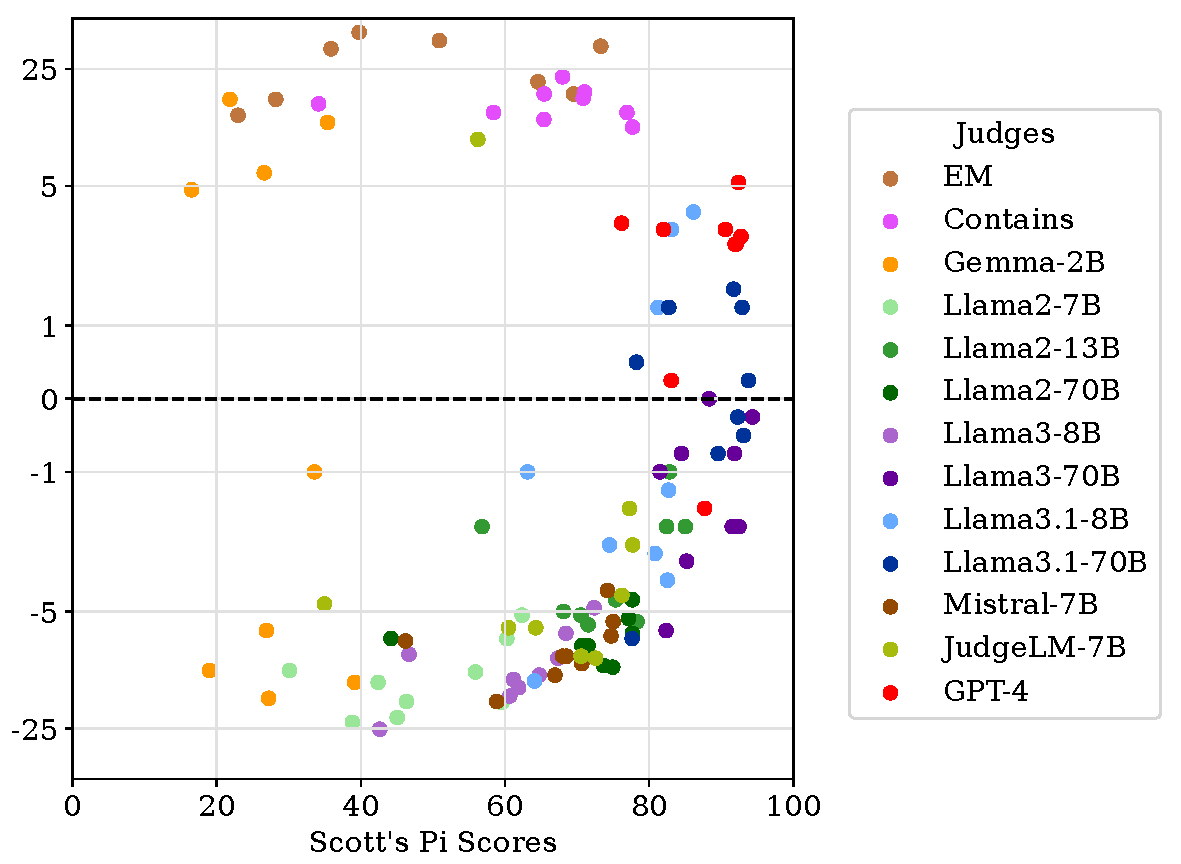
\includegraphics[width=0.9\linewidth]{figures/ScottsPiScoreVariation_bV2.pdf}
        % \vspace{-2mm}
        % \caption{}
        % \vspace{-2mm}
        % \label{fig:pi_vs_delta}
    \end{subfigure}
    \caption{\textbf{Difference with human evaluation scores versus alignment metric.} 
    The delta evaluation score is the difference between the judge and the human score; y-axes are in log scale. 
    Percent alignment (left) shows a very skewwed distribution, making it difficult to distinguish models.
    \scottspi (left) provides a clearer difference between models, and is more indicative of deviation of the gold score.
    % . The left figure shows a skewed distribution for percent agreement and delta evaluation score. Right, we see that highly aligned LLM judges with \scottspi > 0.8 exhibit low variability in scores, while judges with \scottspi < 0.8 demonstrate more variability.
    %impacting their reliability.
    }
    \label{fig:alignment_vs_delta}
\end{figure*}

\paragraph{\Evaluatormodels} \label{subsec:evaluators}
% \subsection{\Evaluatormodels}\label{subsec:evaluators}
%
To understand the strengths and weaknesses of different judges, we consider answers of pre-trained (base) and instruction-tuned (chat) `\evaluatormodels' across a wide variety of model sizes. %, and we examine the quality of the evaluations from different \judgemodels.
In particular, we consider \eval{Llama-2} \citep{touvron2023llama} in 7B, 13B, and 70B parameter sizes for both base and chat versions, \eval{Mistral 7B} \citep{jiang2023mistral} base and chat versions, and \eval{\gpt}\footnote{Accessed via the OpenAI API between Mar 19th, 2024 and Sep 20, 2024.} \citep{achiam2023gpt} as the \evaluatormodels. 
%
The prompts for the \evaluatormodels contain five few-shot examples of (question, answer) pairs from the TriviaQA training set.
The prompts for the instruction-tuned models additionally include a command signaling the model to answer the given question in a succinct manner similar to the provided examples.
The prompts are provided in \cref{app:prompt-templates}.

% \subsection{\Judgemodels} \label{sec:experiments:judgellm}

\paragraph{\Judgemodels}
% \subsection{\Judgemodels}\label{subsec:judges}
%
To get a comprehensive view of the strengths and weaknesses of \judgemodels across different model sizes and architectures, we use instruction-tuned versions of \judge{Llama-2} \citep{touvron2023llama} in 7B, 13B, and 70B sizes, \judge{Llama-3} \citep{meta2024llama3} in 8B and 70B sizes, \judge{Llama-3.1} \citep{dubey2024llama3herdmodels} in 8B and 70B sizes, \judge{Mistral} 7B \citep{jiang2023mistral}, \judge{\gpt} \citep{achiam2023gpt}, \judge{Gemma\;2B} \citep{gemma2024gemma}, and \judge{JudgeLM\;7B} \citep{zhu2023judgelm} as judges. To maintain parity with human and judge evaluation, judge prompts were built from human guidelines in \cref{app:human_annotation_guidelines}. The judges are instructed to respond with only a single word,  \texttt{``correct''} or \texttt{``incorrect''}.
An overview of all \evaluatormodels and \judgemodels is shown in \cref{tab:evaluation}.
For ease of reading, the \judge{\judgemodels} are depicted in a different font than the \eval{\evaluatormodels}.
% \subsection{Evaluation}\label{sec:experiments:baselineandhumanannotation}
% Below, we describe the baselines we compare the \judgemodels with, describe details on how we source human annotations and detail how we compute alignment for the judgemodels.
\paragraph{Baselines} \label{subsec:baselines}
% \subsection{Baselines}\label{subsec:baselines}
As baselines, we use two commonly used lexical evaluation techniques  -- exact match (\judge{EM}) and contains match (\judge{contains}).
For \judge{EM}, a response is considered correct if the response exactly matches one of the reference answers for the given question.
For \judge{contains}, an answer is considered correct if at least one of the reference answers is a sub-string of the response string.
Both EM and contains match are computed in a case-insensitive manner.

% Like exact match evaluation, contains match evaluation is also performed without considering letter casing.
% We compare the judge LLMs assessments with various classical lexical evaluation techniques, such as exact match and contains match, as well as human judgements. In exact match evaluation, if the model's answer exactly matches any of the reference answers for a question, it is evaluated as correct. This evaluation is performed without considering letter casing.
%
% Similarly, contains match evaluation considers an answer correct if the response contains all the words found in any of the reference answers, regardless of their order. Like exact match evaluation, contains match evaluation is also performed without considering letter casing.
%
% The evaluation scores from the judges represent the percentage of questions that the judges deemed correctly answered by the evaluator models, out of the total number of questions in the sample.

\paragraph{Alignment} \label{subsec:alignment}
% \jsubsection{Alignment}\label{subsec:alignment}
We use two metrics to quantify alignment between judges: percent agreement and Scott's Pi coefficient \citep{scott1995scottspi}.%
\footnote{In an earlier version of this paper, we used Cohen's kappa \citep{cohen1960kappa} to measure alignment.
It has since come to our attention that -- despite it's widespread use -- this metric has some well-documented theoretical issues \citep[e.g.][]{pontius2011death,chicco2021matthews}.
For the interested reader, we elaborate on these issues in \cref{app:cohenslimitation}.
}
Percent agreement expresses a simple percentage of the samples on which two annotators agree. 
Scott's Pi, denoted as \scottspi, is an alignment metric that corrects for chance agreement between two annotators and is considered to provide a more robust measure of alignment.
% also takes into account the possibility of chance agreement.
% It is generally considered to provide a more robust measure of alignment. 
Details about the computation of both metrics are given in \cref{app:metrics}.

\begin{figure*}[t]
    \centering
    \begin{subfigure}[b]{0.46\textwidth}
        \centering
        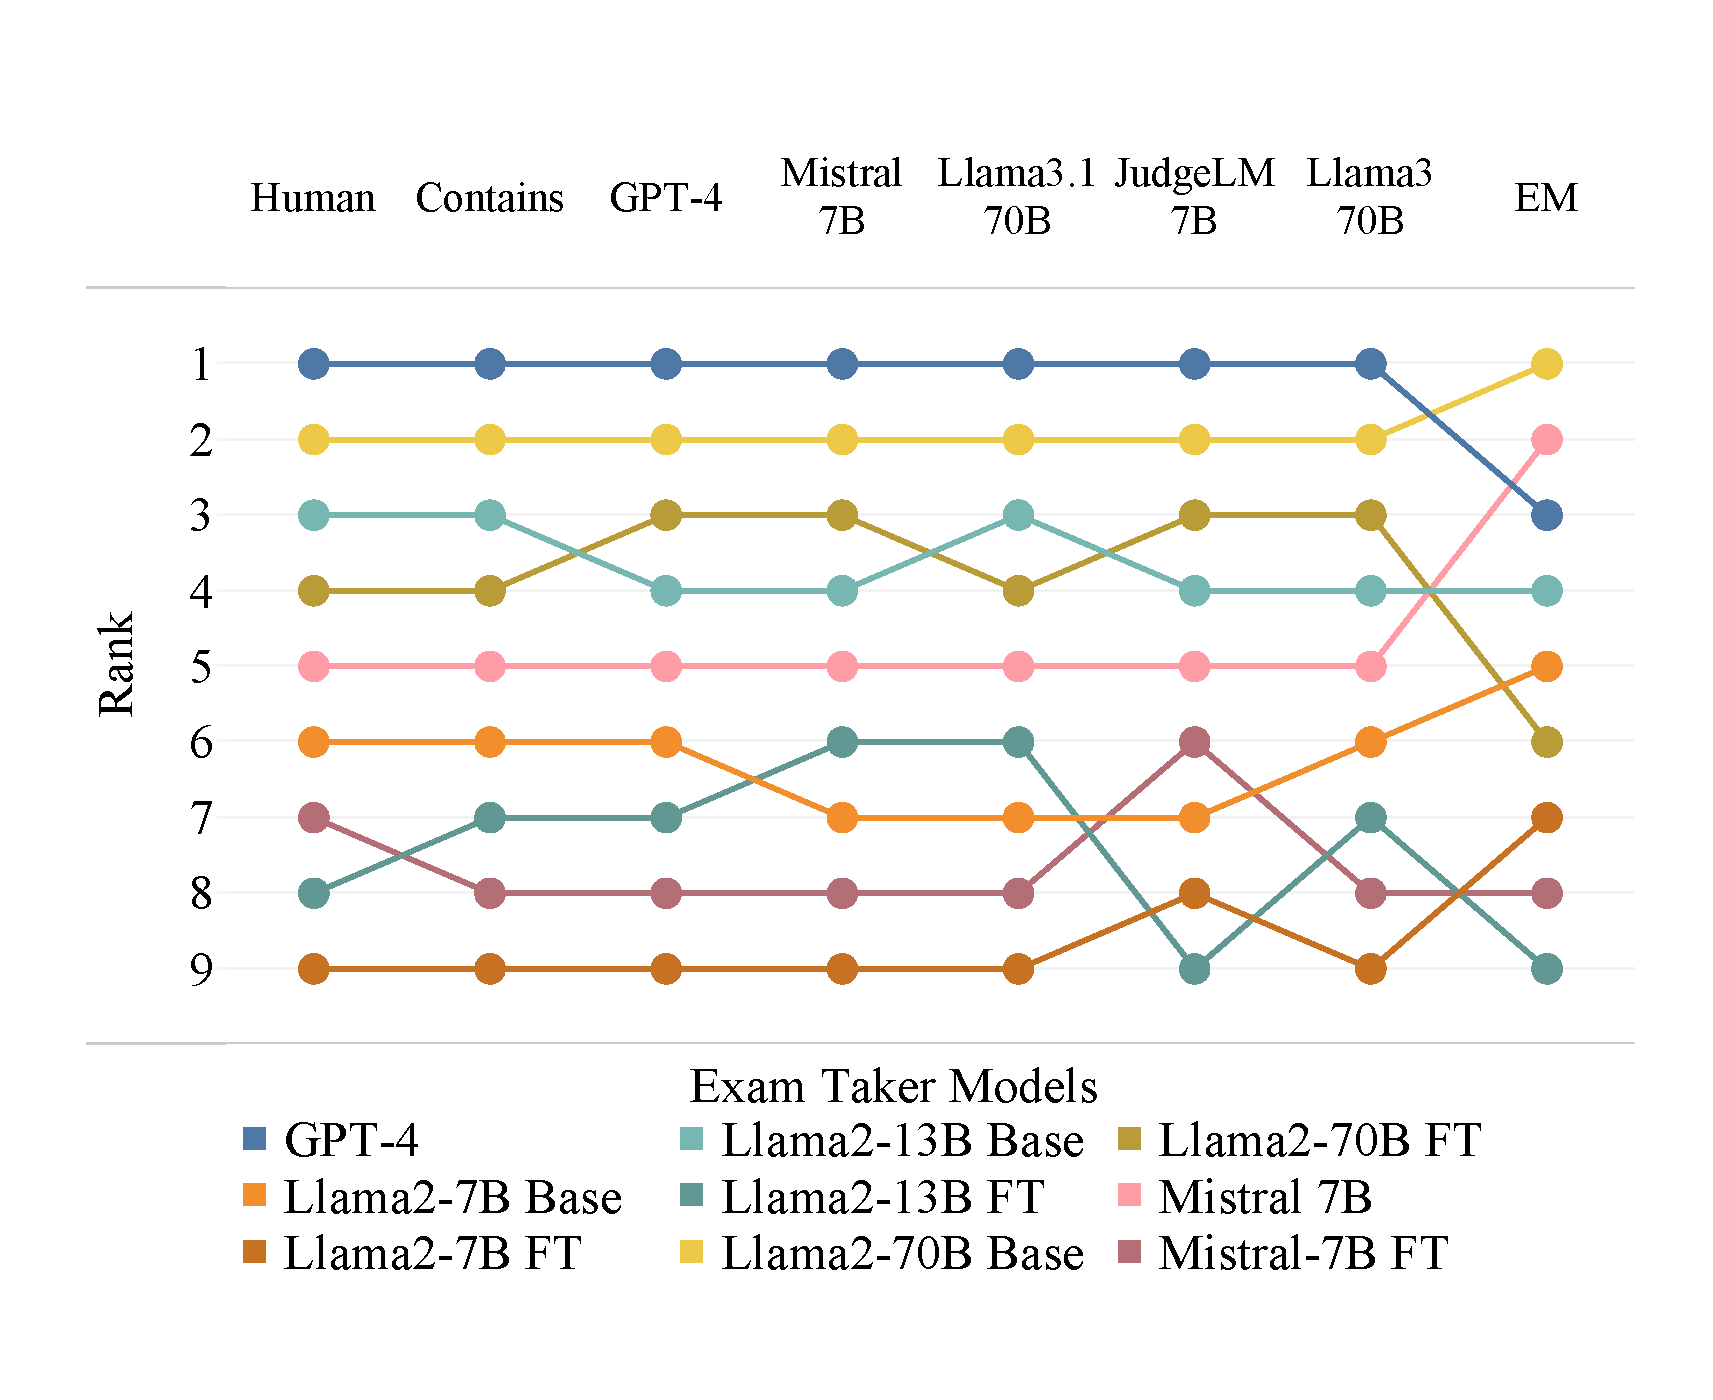
\includegraphics[width=\linewidth]{figures/Rankings_HG.pdf}
        \vspace{-8mm}
        \caption{}
        \vspace{-2mm}
        \label{fig:rankcorrelation}
    \end{subfigure}
    \hfill
    \begin{subfigure}[b]{0.53\textwidth}
        \centering
        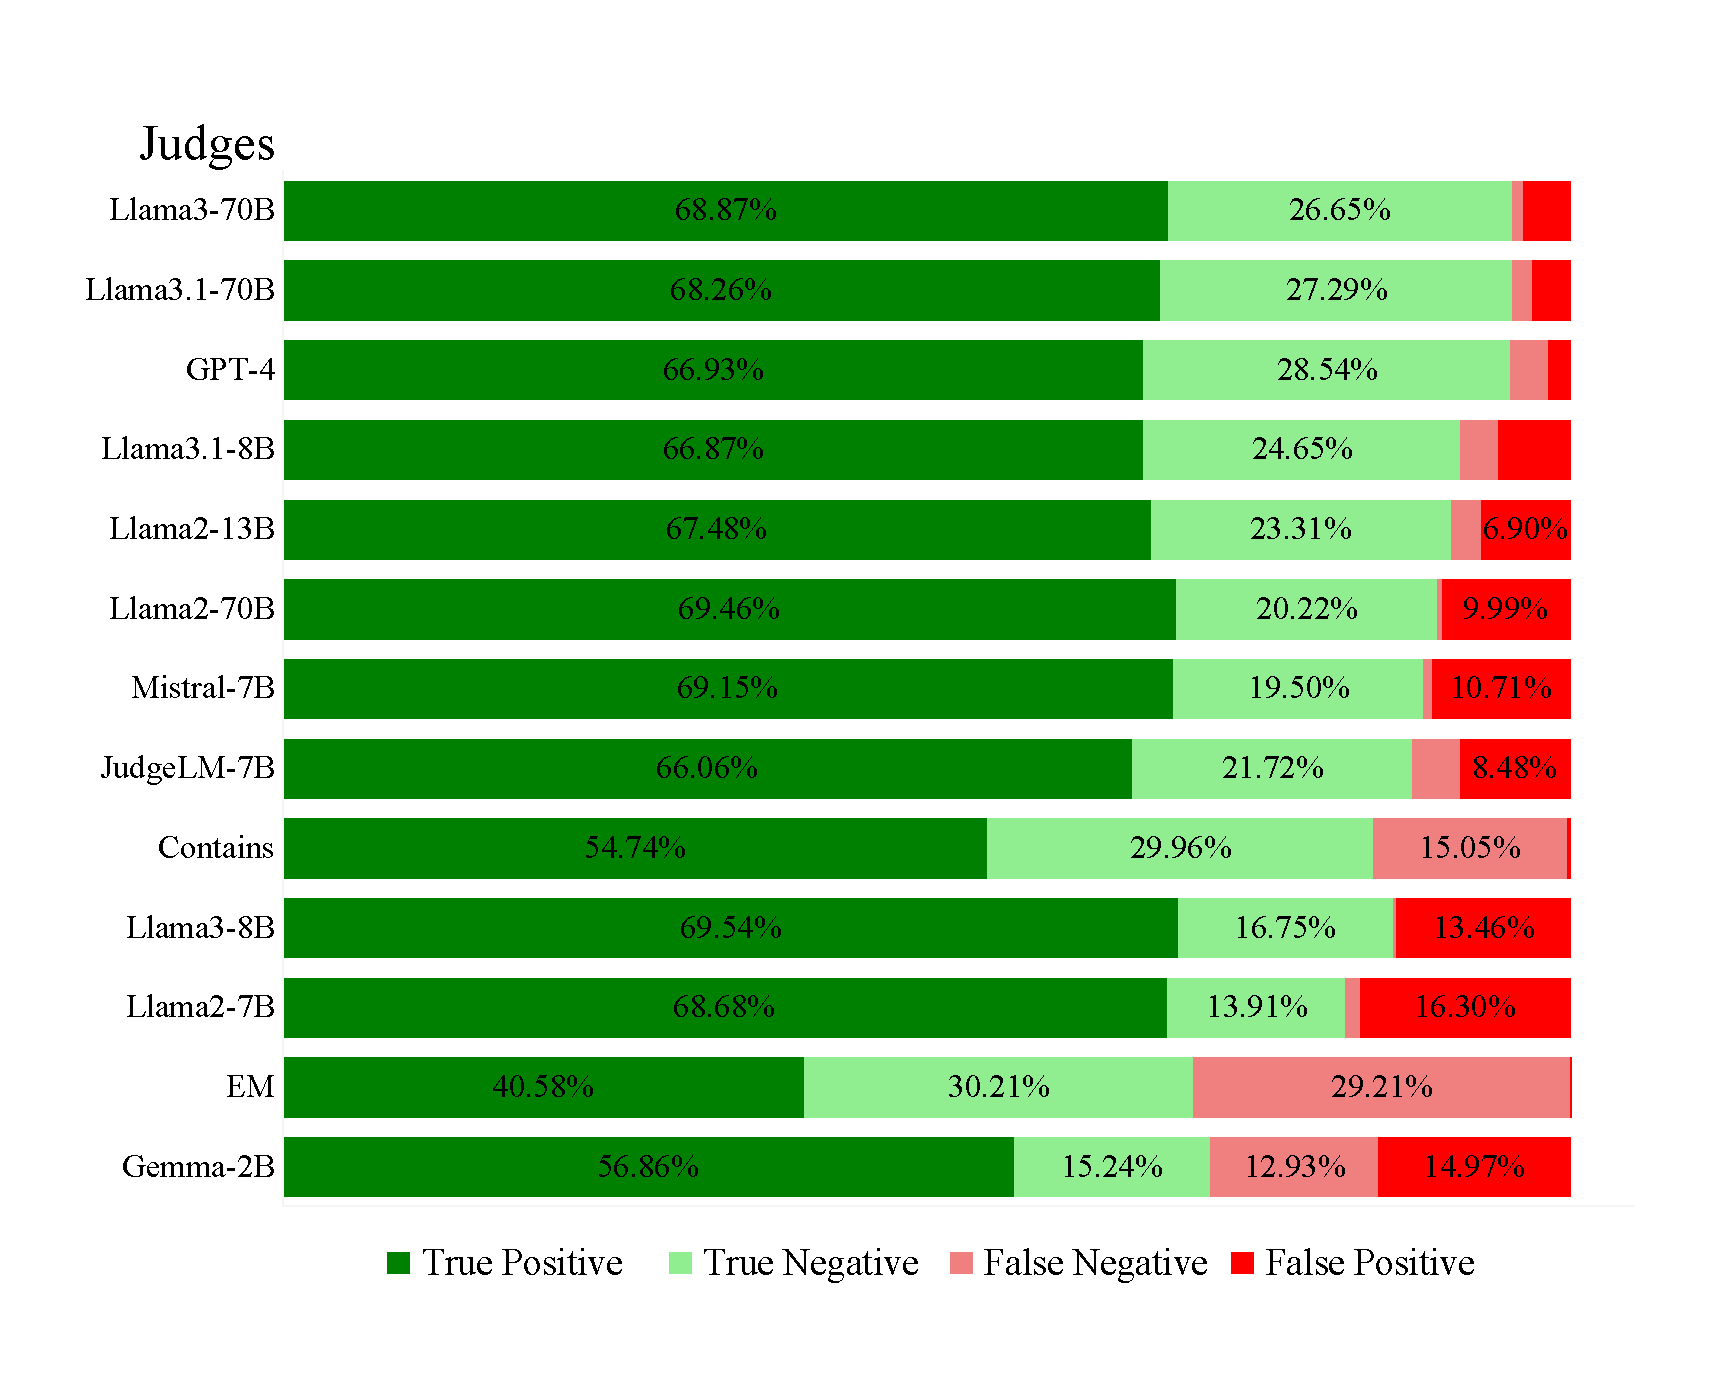
\includegraphics[width=\linewidth, height=5.5cm]{figures/ConfusionMatrixV5.pdf}
        \vspace{-8mm}
        \caption{}
        \vspace{-2mm}
        \label{fig:confusionmatrix}
    \end{subfigure}
    \caption{\textbf{Judge rankings and true/false positives and negatives.} 
    (a) Assigned \evaluatormodel rankings assigned by highly human aligned judges.
    \judge{Contains} stays closely to human-assigned rankings, as well as \judge{\gpt} and \judge{Mistral 7B}. 
    % All judges struggle to distinguish between the poor-performing \evaluatormodels, that may often be closer together.
    (b) False positives and negatives across different \judgemodels, in descending order of human alignment. 
    Both false negatives and false positives increase as human alignment decreases, but well-aligned models tend to produce more false positives than false negatives.
        % \dieuwke{Should increase the font sizes on this one, put the legends on the top and afterwards align appropriately.}
        }\label{fig:ranking_posneg}
\end{figure*}

\paragraph{Human judgements} \label{subsec:human_alignment}
% \subsection{Human judgements}\label{subsec:human_alignment}
As a ground-truth assessment, we obtain human annotations for each \evaluatormodel answer.
The inter-human alignment is calculated between three human judges using the answers to 1200 randomly sampled questions answers; the human guidelines can be found in \cref{app:human_annotation_guidelines}. 
% To compute human inter-annotator agreement, we first conduct an experiment in which three humans judge 600 \eval{Llama-2 7B} \citep{touvron2023llama} answers, randomly sampled from the TriviaQA dataset \citep{joshi2017triviaqa}.
% The human annotators were asked to annotate \evaluatormodel responses that didn't exactly match with one of the references. 
We then determine collective ``Human Judgment'' through a majority vote.
%
% During human annotation, questions marked as correct by the exact match evaluation are skipped, as they are assumed to be annotated correctly by humans. However, these questions are still counted in the final score.

% The average alignment among human evaluators with the majority vote had a \scottspi of $96.2\pm1.07$,%
% \footnote{Coefficient scaled by $100$ for easier comparison with percent alignment.}
% and the average percent agreement was $98.52\%\pm0.42\%$ (pushing the existing SOTA in similar work \citep{zeng2024evaluatinglargelanguagemodels}). 

The average alignment between human evaluators and the majority vote yielded a \scottspi of $96.2\pm1.07$,% 
\footnote{The coefficient is scaled by $100$ for easier comparison with percentage alignment.}
while the average percentage agreement was $98.52\%\pm0.42\%$,  exceeding the alignment previously reported in comparable studies \citep{zeng2024evaluatinglargelanguagemodels}.

The details of this experiment are mentioned in \cref{app:limitations}.
Given this near-perfect alignment score, we consider only one human evaluator per sample for the rest of our experiments, to reduce the overall cost of human annotations. 
The set of questions for which we obtain human annotations is identical for each \evaluatormodel.
%
% After converging on evaluation criteria, we manually annotate 400 questions for each evaluation model.
% Given the high cost of human annotations and near-perfect human alignment between annotators, each evaluation model is annotated by only one human annotator for 400 random sample. 


%\kc{better name?} 
%  We focus on the case of binary annotation, where each evaluation is one of two possible values (e.g., \texttt{correct} or \texttt{incorrect}). 
%  



\section{Results} \label{sec:results}

% \setlength{\textfloatsep}{10pt}
In this section we discuss our main results, primarily focusing on the relationship between evaluations by various \judgemodels and human evaluations (\cref{sec:results:exploringhumanjudgellmalignment}), and how that impacts their usability (\cref{sec:results:exploringsystematicpatterns}).
To do so, we evaluate their alignment with human judgment and assess how differently they rank the \nexamtakersword \evaluatormodels compared to humans.
In Section \ref{sec:analysis}, we further analyse their precision and recall to further investigate the types of errors that can be made by various \judgemodels. Details about compute requirements and others costs for experiments are given in \cref{app:experiment-costs}.

% \subsection{How well are various judges aligned with humans?}
\subsection{Alignment between \judgemodels and humans}
% \subsection{Human - \JudgeModel Alignment}
\label{sec:results:exploringhumanjudgellmalignment}

We start by computing \scottspi scores and percent agreement between the evaluations of each \judgemodel and the human annotators. %for all \evaluatormodels. 
We show the result in \cref{fig:llmalignment}.
We observe that percent alignment is high for virtually all models, with the exception of \judge{Gemma\;2B} and \judge{EM}.
\scottspi, on the other hand, has low values for most models, though its value is in the high 80s for \judge{Llama-3\;70B}, \judge{Llama-3.1\;70B}  and \judge{\gpt}. %  have \scottspi scores -- 88, 88 and 87, respectively -- that are considered to indicate excellent alignment.
Nevertheless, there still is a significant disparity between human judgment and \judgemodels: the best scoring judge, \judge{Llama-3\;70B}, is 8 points behind human judgment. 
Notably, \judge{EM} has the most variance in alignment, while \judge{Gemma\;2B} has the lowest alignment amongst all judges.
% \sout{Notably, \judge{contains} has a higher \cohenskappa score than half of the \judgemodels}, while \judge{EM} has the lowest alignment among all judges. 

% \paragraph{\scottspi vs percent agreement}

In most cases, we observe that \scottspi and percent agreement are following the same trend, with the exception of the values for \judge{Gemma\;2B} and \judge{EM}.
\judge{Gemma\;2B} shows higher percent agreement compared to \judge{EM}, yet it yields the lowest \scottspi score within the ensemble.
% Furthermore, there is a significant difference in the actual values.
For the percent agreement of judge models, we note a 26-point difference between human judgment and EM, while \scottspi exhibits a more substantial 64-point gap. 
This is also visible in the general decline of alignment scores: while \judge{Llama-3\;8B} has a \scottspi score of only 59, its percent agreement is still well above 80\%.
Overall, \scottspi appears to be better able of discriminating various judge models, showing more divergence across the tested judges.
% From \cref{fig:llmalignment_b}, we can also observe that the greater the deviation of judges from human judgments, the more significant the variation in their \cohenskappa scores becomes.

To understand how indicative the two alignment metrics are of the expected accuracy of the overall judgement of the models, we plot, for each \judgemodel and \evaluatormodel, the difference between the score assigned by the judge and the score assigned by a human.
In the figure, we can see that for \scottspi values higher than 80, the evaluation scores are comparatively close to the human evaluation scores, with a difference of up to 5 points in their assigned scores (complete results table provided in \cref{app:all_scores}). % TODO check!
For percent alignment, on the other hand, even judges that have more than 90\% may still differ more than 10 points in their assigned score.
% 
% \paragraph{Alignment vs assigned score}
% In \cref{fig:cohenskappa}, we show the variation in scores assigned by the \judgemodels to various \evaluatormodels for different values of percent agreement (\cref{fig:cohenskappa_part1}) and Scott's pi (\cref{fig:cohenskappa_part2}).
% To get a better idea of how much variation in actual assigned scores can be expected given a particular kappa, we plot the differences between scores provided by judges and those from human assessment across a range of judge kappa scores, in \cref{fig:cohenskappa} (assigned scores per model can be found in \cref{fig:llmalignment_a}).
% \dieuwke{TODO: make y-axis log-scale}.
%\sout{
% We can see that for \scottspi > 80, the evaluation scores by \judgemodels are close to the human evaluation scores for most of the judges, with a difference of up to 5 points in their assigned scores (complete results table provided in \cref{app:all_scores}).
%}
% For percent agreement we observe deviations of up to 20 points in the evaluation scores for similar scott's pi alignment.
Interestingly, %, for several \judgemodels, 
the deviation from human-judgements for a single judge model can be quite different depending on the \evaluatormodel.
% is quite distinct for different \evaluatormodels.
In \cref{fig:llmalignment_a}, \judge{Gemma\;2B}, for instance, sometimes assigns higher scores than humans, and sometimes much lower. 
In the next section, we further explore this particular pattern.

% \subsection{How does this impact their usability?}
\subsection{Exploring consistent patterns in \judgemodels} \label{sec:results:exploringsystematicpatterns}

% \begin{figure}[h]
%     \centering
%     \includegraphics[width=\linewidth]{figures/JudgeScoreforExamTakers.png}
%     \caption{ We plot the delta between Judge exam scores and human assessment for various exam takers.Judge LLMs exhibit diverse distributions and rankings across different exam-taker, none of which exactly mirror the assessments of human judges. However, well aligned tend to consistently score more than the human assessment. \dieuwke{Invert this so that i) the exam taker models are on the y-axis, and the colour indicates the judges, and ii) put the actual score, not the delta.} \dieuwke{Potentially: put next to the figure with the rankings.}}
%     \label{fig:assigned_scores}
% \end{figure}


In the previous section, we saw that none of the \judgemodels were as aligned with humans as humans were with each other. As shown in \cref{fig:alignment_vs_delta}, even the best-aligned \judgemodels can differ by up to 5 points from human-assigned scores. While this limits their ability to perfectly estimate \evaluatormodel capabilities, \judgemodels can still provide valuable insights to \textit{differentiate} between \evaluatormodels. For example, judges with consistent biases may not assign identical scores but could rank models similarly, akin to a very strict teacher.

To assess this, we compare the rankings given by each \judgemodel to the nine \evaluatormodels, computing Spearman's rank correlation coefficients $\rho$ \citep{spearman1904spearman} with the human ranking. The rankings are shown in \cref{fig:rankcorrelation}, with $\rho$ and $\sigma$ values in \cref{app:correlationcoefftable}. Most \judgemodels have rank correlations above 0.7, indicating they struggle to distinguish poorer models but do well with better ones. Notably, models like \judge{contains} and \judge{Mistral 7B}, which have divergent scores from humans, show high rank correlation ($\rho$ of 0.99 and 0.98, respectively), performing similarly to \judge{\gpt} and outperforming the better \judge{Llama} models -- though with lower significance values -- indicating that identifying which models are better should not be equated to assigning them the correct score.

% In the previous section, we have seen that none of the \judgemodels we considered were aligned with humans as well as the humans were aligned amongst themselves.
% Furthermore, as can be seen in \cref{fig:alignment_vs_delta}, the scores assigned by even the best aligned \judgemodels can differ up to 5 points with the human-assigned scores.
% However, while this may limit -- to some extent -- the utility of using a \judgemodels to get a perfect estimate of the \evaluatormodel's capability on the benchmark, the \judgemodels may still offer valuable insights to \textit{differentiate} between different \evaluatormodels.
% %For example, 
% If judges exhibit consistent biases such as -- akin to a very strict teacher -- consistently rating any \evaluatormodel lower, they will not assign identical scores but may assign identical \textit{rankings}.

% To evaluate this, we compare the rankings assigned by each \judgemodel to the nine \evaluatormodels by computing their Spearman's rank correlation coefficients $\rho$ \citep{spearman1904spearman} with the human ranking. 
% We show the rankings in \cref{fig:rankcorrelation}, with $\rho$ and corresponding $\sigma$ values in \cref{app:correlationcoefftable}. 
% Most \judgemodels have rank correlations higher than 0.7; it appears they struggle to distinguish between poorer-performing \evaluatormodels, but do well at distinguishing between better-performing ones.
% Notably, the results show that several models that assign scores quite divergent from humans and have poor alignment on the sample level are very aligned in terms of the rankings they assign.
% Specifically, both \judge{contains} and \judge{Mistral 7B}, with \scottspi values of 64 and 66, respectively, exhibit very high rank correlation with the human scores ($\rho$ 0.99 and 0.98, respectively, with $\sigma$ 0.02 and 0.03).
% With that, these judges perform on par with \judge{\gpt} and outperform the better \judge{Llama} judges -- though with lower significance values -- indicating that identifying which models are better should not be equated to assigning them the correct score.


% Generally, even smaller judges appear to be good at distinguishing higher performing models, but struggle more when performance is lower.

% These results show that \judge{contains} demonstrates the highest alignment with the human ranking, swapping the ranks of only two out of nine models. 
%\sout{
% Notably, \judge{contains} performs on par with \judge{\gpt} and \judge{Mistral 7B}, the judges with the best alignment.
% Most \judgemodels have rank correlations higher than 0.7; it appears they struggle to distinguish between poorer-performing \evaluatormodels, but do well at distinguishing between better-performing ones.
% We see that all best-aligning judges are consistent in their ranking of the top two models: they all agree that, of the models evaluated, GPT4 is the best performing model, followed by Llama2-70b-base.
% Below the top two, there are more changes.
% The GPT-4 and Llama3 have the same three models in spot three, four and five as the human judge, but both with different orders.
% Generally, judges appear worse at distinguishing poorer performing models than better-performing models.

% Classical lexical models fare even worse with greater misalignment with human judgement across the board, with the -- commonly used -- EM score not even agreeing on the top-performing model.


% \begin{table}[h]
%     \centering
%     \begin{tabular}{|c|c|}
%     \hline
%     \textbf{Model} & \textbf{Spearman Rank Correlation Coeff} \\
%     \hline
%     Human Alignment & 100 \\
%     GPT-4 & 99.17 \\
%     Llama3-70B & 99.17 \\
%     Llama-70B & 81.67 \\
%     Mistral-7B & 77.50 \\
%     Contains & 41.67 \\
%     Llama-7B & 85.00 \\
%     Llama3-8B & 42.50 \\
%     JudgeLM-7B & 59.17 \\
%     Llama-13B & 18.33 \\
%     EM & 65.83 \\
%     Gemma-2B & 48.33 \\
%     \hline
%     \end{tabular}
%     \caption{Judges sorted by Kappa Human Alignment and their Spearman Rank Correlation Coeff}
%     \label{tab:scores_multiplied}
% \end{table}

% \begin{figure}[h]
%     \centering
%     \begin{minipage}[b]{0.49\textwidth}
%         \centering
%         \includegraphics[width=\linewidth]{figures/InterLLMAlignment.png}
%         \caption{Inter Judge Alignment}
%         \label{fig:interllmalignment}
%     \end{minipage}
%     \hfill
%     \begin{minipage}[b]{0.49\textwidth}
%         \centering
%         \includegraphics[width=\linewidth]{figures/RankCorrelationCoeff.png} 
%         \caption{Judge Ranking over Evaluation Models}
%         \label{fig:rankcorrelation}
%     \end{minipage}
% \end{figure}

% \subsubsection{Precision, Recall \& False Positives}

% Using the human judgement, we calculate the precision, recall and false positive rate to quantify judge LLM performance. To understand the precision-recall tradeoff, we plot the precision and recall rates and maintain The ordering of LLMs from Figure \ref{fig:llmalignment}. We can observe in figure \ref{fig:precisionrecall}, when LLMs become more aligned with human judgment, their recall improves. Precision, on the other hand, remains relatively consistent across all LLMs due to balancing effect of increase in true positive and false positives. From figure \ref{fig:confusionmatrix}, we can observe increase in true positives but not a similar reverse trend in False Positive. Instead, we see that the False Negatives are decreasing with increase in human alignment for Judges. 

% \begin{figure}[h]
%     \centering
%     \begin{minipage}[b]{\textwidth}
%         \centering
%         \includegraphics[width=\linewidth]{figures/PrecisionRecall_V4.png}
%         \caption{Precision \& recall with increasing human alignment}
%         \label{fig:precisionrecall}
%     \end{minipage}
% \end{figure}

% \begin{figure}[h]
%     \centering
%     \begin{minipage}[b]{\textwidth}
%         \centering
%         \includegraphics[width=\linewidth]{figures/ConfusionMatrixV2.png}
%         \caption{Judge performance \& error rate with increasing human alignment }
%         \label{fig:confusionmatrix}
%     \end{minipage}
% \end{figure}




% To explore the variability in scores among LLMs within the same cluster, we focus on the first group comprising Llama2-80B, Llama3-80B, Mistral-7B, and GPT-4, plotting their evaluation scores. Figure Y illustrates that despite similar Kappa scores for identical questions and evaluation models, judges' responses yield disparate evaluator results. In the worst-case scenario, these results can differ by up to 10 points

% \begin{figure}[h]
%     \centering
%     \begin{minipage}[b]{\textwidth}
%         \centering
%         \includegraphics[width=\linewidth]{figures/VariationofScores.png}
%         \caption{Variation of Scores for similar Kappa Scores}
%         \label{fig:llmalignment}
%     \end{minipage}
% \end{figure}

% In our study, we investigated nine evaluation models and anticipated consistency in the ranking of judges across each model. To verify this assumption, we assessed the ranking of each judge across the different evaluation models. Recognizing the possibility of unchanging rankings (no variance), we computed and plotted the Spearman Rank Correlation Coefficient (cite) across the 12 judges. Spearman Rank Correlation is valuable as it gauges the degree to which the relationship between two variables can be described using a monotonic function. A Spearman Rank Correlation exceeding 0.7 indicates a strong correlation, a common occurrence in robust benchmarks. However, the plotted data in Figure (cite) reveals fluctuations in rankings among the remaining evaluators.

% \begin{figure}[h]
%     \centering
%     \includegraphics[width=0.6\textwidth]{figures/score-kappa-0.png}
%     \caption{Scores assigned by different evaluators vs their alignment with human evaluations}
%     \label{fig:score-kappa-0}
% \end{figure}

% \begin{figure}[h]
%     \centering
%     \includegraphics[width=0.6\textwidth]{figures/score-kappa-1.png}
%     \caption{Scores assigned by different evaluators vs their alignment with human evaluations}
%     \label{fig:score-kappa-0}
% \end{figure}

% \begin{figure}[h]
%     \centering
%     \includegraphics[width=0.6\textwidth]{figures/score-kappa-2.png}
%     \caption{Scores assigned by different evaluators vs their alignment with human evaluations}
%     \label{fig:score-kappa-0}
% \end{figure}





% OLD STUFF


% \begin{figure}[h]
%     \centering
%     \includegraphics[width=\textwidth]{figures/humanalignment_withem.png}
%     \caption{Human Alignment w GT}
%     \label{fig:human}
% \end{figure}

% \begin{table}[h]
%     \centering
%     \caption{Percentage Alignment}
%     \label{tab:my_table}
%     \begin{tabular}{cccccc}
%         \toprule
%         \textbf{Scenario} & \textbf{Avg Alignment} & \textbf{Human-A} & \textbf{Human-S} & \textbf{Human-K} & \textbf{Avg Size} \\
%         \midrule
%         All Questions & 98.33 & 97.33 & 98.5 & 99.17 & 600 \\
%         Low Confidence & 98.92 & 99.51 & 97.7 & 99.53 & 214 \\
%         High Confidence & 98.05 & 96.22 & 98.95 & 98.96 & 386 \\
%         \bottomrule
%     \end{tabular}
% \end{table}

% \begin{table}[htbp]
%     \centering
%     \begin{tabular}{cccccc}
%         \toprule
%         \textbf{Scenario} & \textbf{Avg Alignment} & \textbf{Human-A} & \textbf{Human-S} & \textbf{Human-K} & \textbf{Avg Size} \\
%         \midrule
%         All Questions & 96.75 & 94.81 & 97.08 & 98.38 & 308 \\
%         Low Confidence & 98.92 & 99.51 & 97.71 & 99.53 & 214 \\
%         High Confidence & 92.34 & 85.71 & 95.56 & 95.74 & 94 \\
%         \bottomrule
%     \end{tabular}
%     \caption{Without EM - Percentage Alignment}
%     \label{tab:my_table2}
% \end{table}

% \begin{table}[htbp]
%     \centering
%     \caption{Kappa Scores}
%     \label{tab:my_table2}
%     \begin{tabular}{cccccc}
%         \toprule
%         \textbf{Scenario} & \textbf{Avg Kappa} & \textbf{Human-A} & \textbf{Human-S} & \textbf{Human-K} & \textbf{Avg Size} \\
%         \midrule
%         All Questions & 96.36 & 94.14 & 96.75 & 98.19 & 600 \\
%         All Questions - EM & 92.38 & 88.06 & 92.96 & 96.13 & 600 \\
%         \bottomrule
%     \end{tabular}
% \end{table}

% \begin{figure}[h]
%     \centering
%     \includegraphics[width=0.8\textwidth]{figures/HumanHeatMap.png}
%     \caption{Human Alignment with Kappa Scores}
%     \label{fig:human}
% \end{figure}

\section {Analysis}\label{sec:analysis}

\begin{figure*}[t]
    \centering
    \begin{subfigure}[b]{0.48\textwidth}
        \centering
        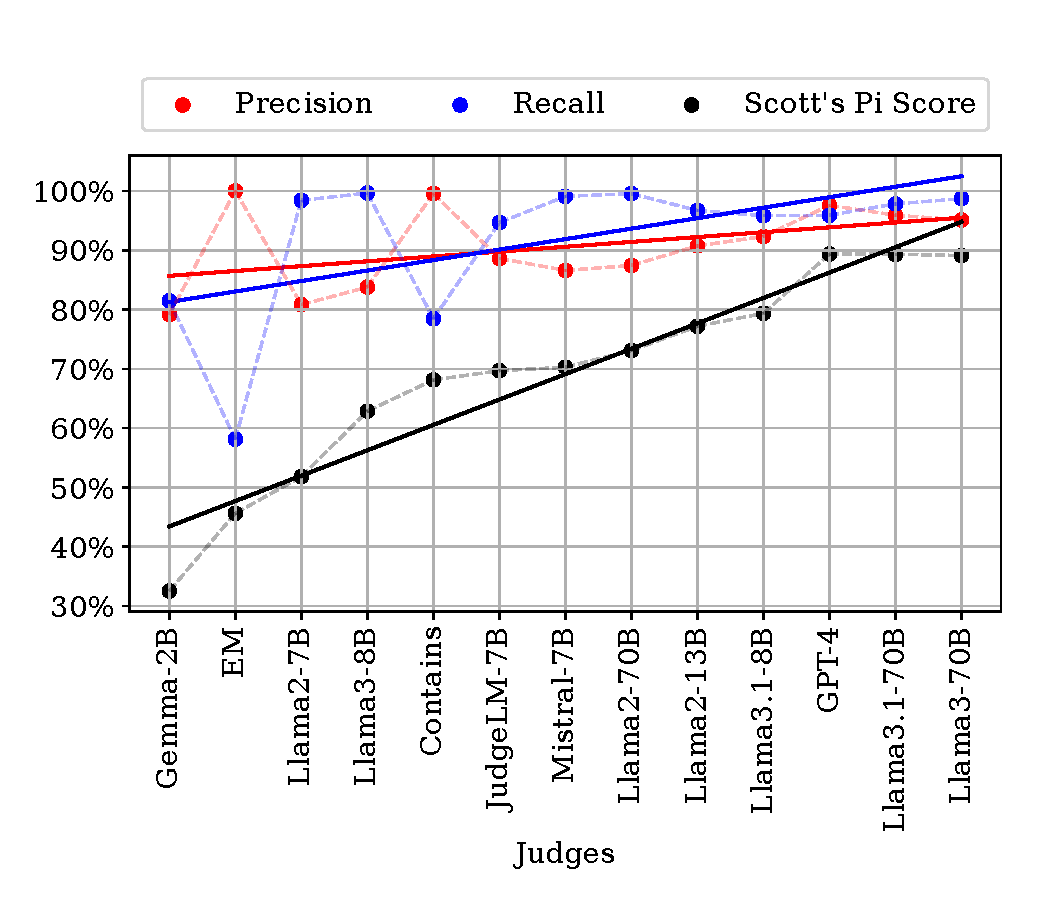
\includegraphics[width=\linewidth]{figures/PrecisionRecall_V6.pdf}
        \vspace{-6mm}
        \caption{}
        \vspace{-2mm}
        \label{fig:precisionrecall}
    \end{subfigure}
    \hfill
    \centering
    \begin{subfigure}[b]{0.51\textwidth}
        \centering
        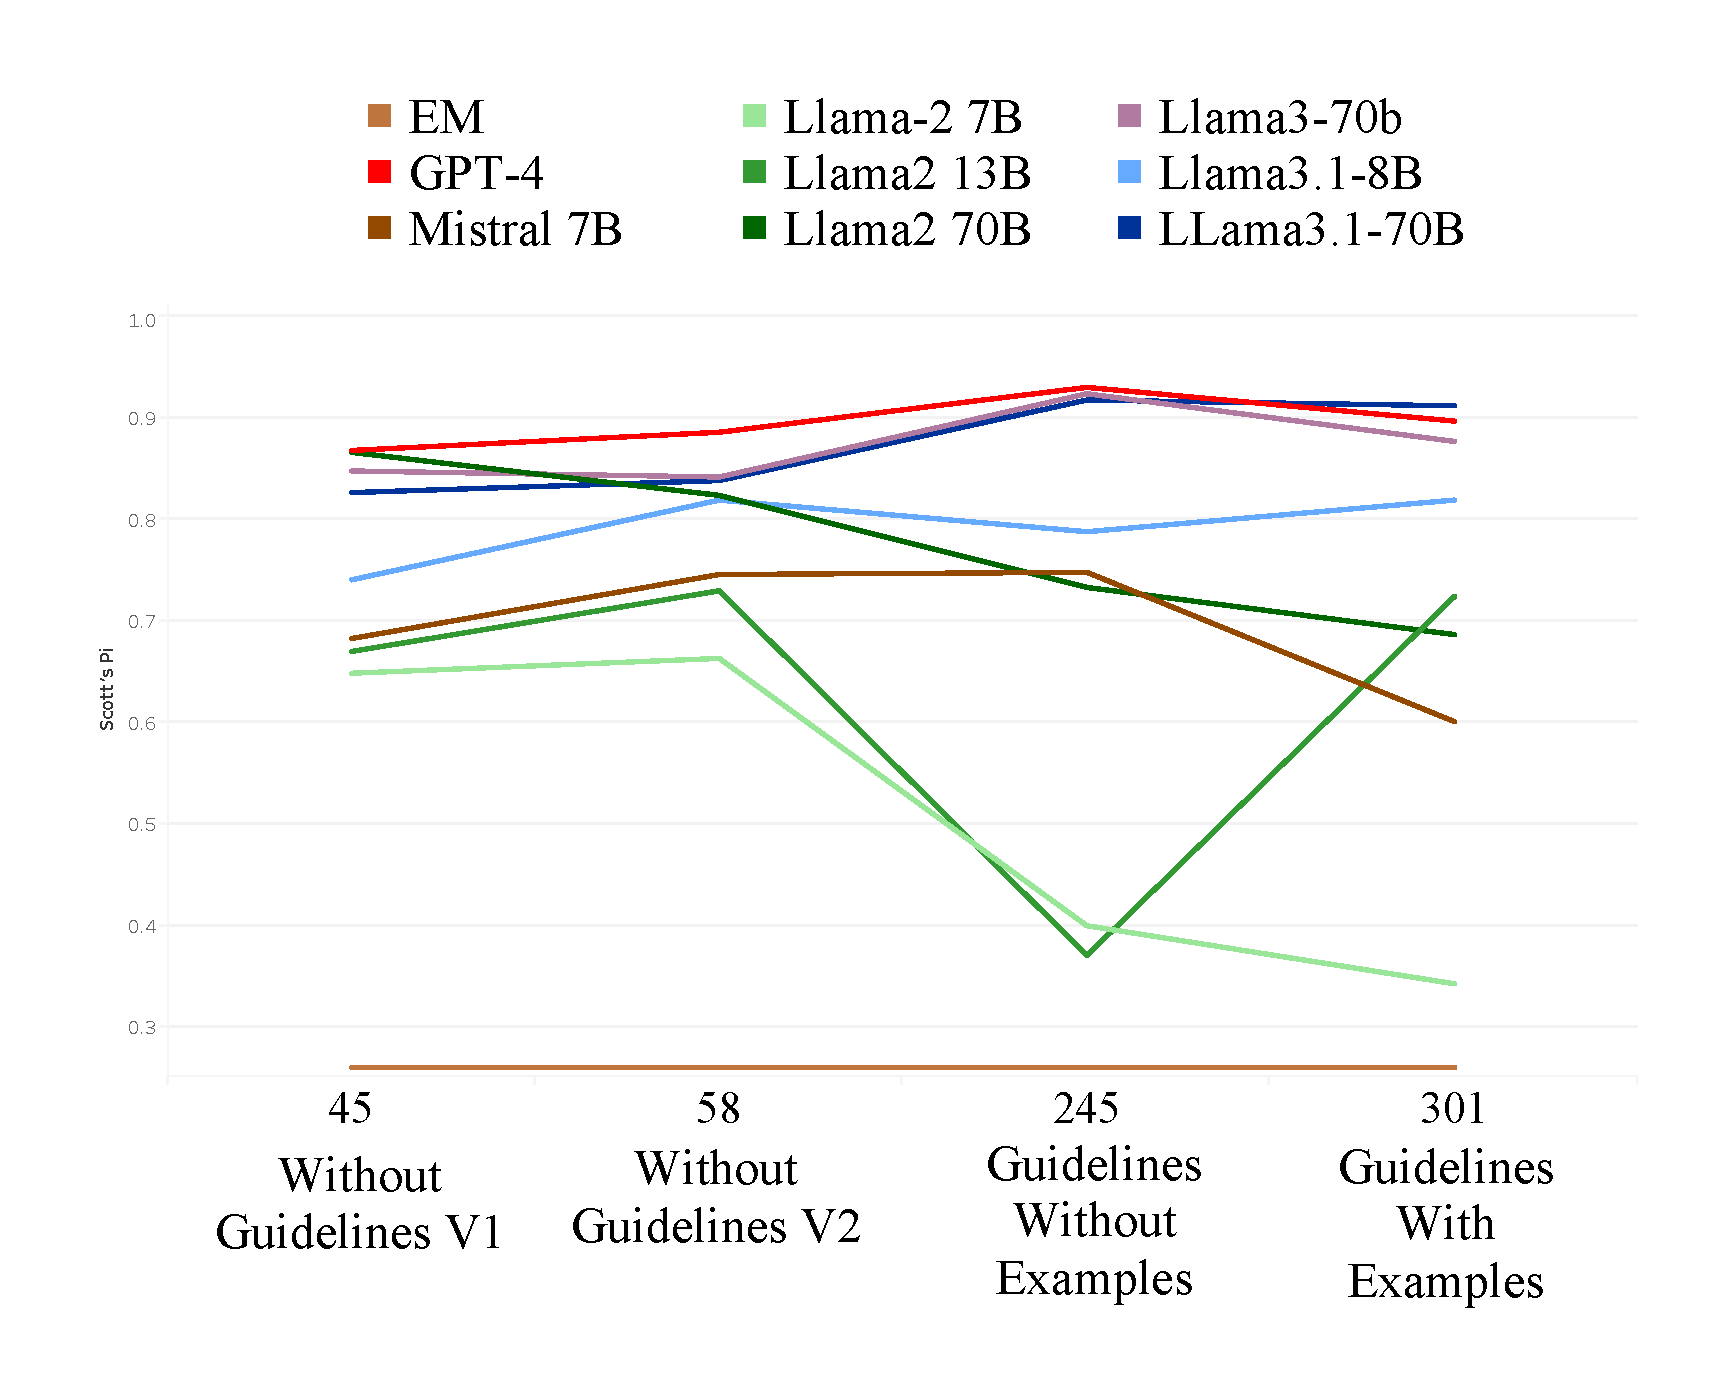
\includegraphics[width=\linewidth]{figures/TooMuchInfo.pdf}
        \vspace{-6mm}
        \caption{}
        \vspace{-2mm}
        \label{fig:TooMuchInfo}
    \end{subfigure}
    
% This adds space between the subfigures
    \caption{\textbf{Precision, recall and prompt sensitivity.} (a) Recall and precision improve with increasing human alignment (\( R^2 \) = 0.31 and \( R^2 \) = 0.21, respectively). %(\( R^2 \) = 0.91). 
    (b) \scottspi scores for judges across different instructions. 
    }
\end{figure*}

\begin{table*}[t]
% \captionsetup{skip=8pt} % Adjust space between table and caption
\resizebox{\textwidth}{!}{
    \begin{tabular}{lllllll}
        \textbf{Error code} & \textbf{Explanation} & \textbf{Example} & \textbf{Proportion} & \textbf{GPT-4 recall} & \textbf{Llama-3 70B recall}\\ 
        \toprule\toprule
        \textbf{Incorrect entity} & \specialcell{Response refers to a wrong entity} & \specialcell{\texttt{Henry VII, James I, Edward VI,} \\ \texttt{Mary I and Elizabeth I}} & 86.9\% & \textbf{98.3\%} & \textbf{96.6\%}\\
        \hline
        \textbf{Under-specified} & \specialcell{Response contains only part \\ of the answer} & \specialcell{\texttt{Henry VII, Henry VIII, Edward,} \\ \texttt{Mary, and Elizabeth}} & 37.3\% & 33.9\% & 23.3\% \\
        \hline
        \textbf{Too few entities} & \specialcell{Response contains too few entities} & \specialcell{\texttt{Henry VII, Edward VI,} \\ \texttt{Mary I and James I}} & 2.47\% & \textbf{80.0\%} & 60.0\%\\
        \hline
        \textbf{Too many entities} & \specialcell{Response contains too many entities} & \specialcell{\texttt{Henry VII, Henry VIII, Edward VI,} \\ \texttt{Mary I, James I, and Elizabeth I}} & 2.7\% & \textbf{90.1\%} & \textbf{90.1\%} \\
        \hline
        \textbf{Other} & \specialcell{Response is incorrect but cannot \\ be put into any of the above buckets} & \specialcell{\texttt{I'm sorry but I do not know the} \\ \texttt{answer to that question}} & 1.23\% & 20.0\% & 40.0\% \\
        \bottomrule
    \end{tabular}
    }
     \caption{\textbf{Error analysis for \judge{GPT-4} and \judge{Llama-3 70B} judges.} 
     %Error codes used to identify the types of errors made by \evaluatormodels when answering questions. 
     The example question is \textit{``Excluding Lady Jane Grey, who were the five monarchs of the House of Tudor?''}, the correct answer \textit{``Henry VII, Henry VIII, Edward VI, Mary I and Elizabeth I''} (in any order).}
     \label{table:error_codes}
\end{table*}

To better understand the \judgemodels, we conduct multiple case studies aimed at identifying common errors and vulnerabilities in the judges we investigate.
Specifically, we study their precision and recall and error types (\cref{sec:analysis:subsec:precision_recall}), their sensitivity to the instruction prompt prompt (\cref{sec:analysis:subsec:instructions}), how they respond to controlled resposes of specific types (\cref{sec:analysis:subsec:judge-ability}), and the extent to which they have a \textit{leniency bias} (\cref{sec:leniency-bias}).
% We study the precision and recall of the \judgemodels and their ability to recall specific error types (\cref{sec:analysis:subsec:precision_recall}), how sensitive \judgemodels are to the length of prompts and the clarity of guidelines (\cref{sec:analysis:subsec:instructions}), ability of judges to evaluate controlled responses (\cref{sec:analysis:subsec:judge-ability}), the leniency of \judgemodels in grading (\cref{sec:leniency-bias}) and the difference in evaluation of base and chat \evaluatormodels (\cref{app:BaseVsChatSupp}).
%\dieuwke{insert rest of the results}.

\subsection{Better aligned models: Precision and recall gains with error spotlights}
\label{sec:analysis:subsec:precision_recall}

We first examine the precision and recall of the \judgemodels. As shown in \cref{fig:precisionrecall}, both metrics increase moderately with alignment. \cref{fig:confusionmatrix} reveals a similar trend, with a clearer distribution of false positives and negatives. True positives remain consistent across varying judge quality, whereas true negatives exhibit a slight decline as judge quality decreases. Notably, a reduction in judge quality leads to an increase in false positives.

% True positives remain stable across many judges, while true negatives decrease as judge quality drops, indicating it's easier to identify correct answers.

Next, we analyze the errors made by \judgemodels by manually annotating 900 outputs from \eval{Llama-7B Base}, focusing on top performers \judge{\gpt} and \judge{Llama-3;70B}. We categorize error types and determine how often they are correctly judged as incorrect. The results in \cref{table:error_codes} show that both \judge{\gpt} and \judge{Llama-3;70B} excel at identifying answers referring to incorrect entities or containing too many entities. Under-specified and incorrect answers are more challenging, with \judge{\gpt} performing better on answers with fewer entities than \judge{Llama-3;70B}.

% We first investigate the precision and recall of the \judgemodels. 
% Maintaining the ordering of \cref{fig:llmalignment}, we plot both in \cref{fig:precisionrecall}. 
% We can see that both precision and recall exhibit a moderate increasing trend as alignment increases. 
% In \cref{fig:confusionmatrix}, we observe a similar pattern, though with a clearer picture on the distribution of false positives and negatives.
% Specifically, we see that the number of true positives is quite stable across many judges.
% The true negatives, instead, drop off quickly as the judge quality decreases, suggesting it is generally easier to judge answers that are correct.

% there is a similar pattern to observe; a sharp decline in false positives initially, along with a gradual decline in false negatives.

% It can be seen that the precision shows moderate r observable trend with increasing alignment, which can be further observed in \cref{fig:confusionmatrix}.
% The recall, \sout{on the other hand}, shows an increasing trend, with more aligned models having comparatively fewer false negatives.

% \begin{figure}[h]
%     \centering
%         \includegraphics[width=\linewidth]{figures/ConfusionMatrixV2.png}
%         \caption{Judge performance \& error rate with increasing human alignment }
%         \label{fig:confusionmatrix}
% \end{figure}

% \subsection{What types of errors do \judgemodels recall?}\label{sec:analysis:subsec:error_analysis}

% Next, we analyse the types of errors made by the \judgemodels by manually annotating 900 outputs from \eval{Llama-7B Base} with error codes, focusing on the top performers \judge{\gpt} and \judge{Llama-3\;70B}.
% We then determine the percentage of each error type that are correctly judged to be incorrect by these two models.
% The results are shown in \cref{table:error_codes}, where it can be observed that both \judge{\gpt} and \judge{Llama-3 70B} have a good error recall when the answers refer to an incorrect entity, or when too many entities are present.
% Under-specified and otherwise incorrect answers are most challenging for both judges, while answers with too few entities are judged relatively accurately by \judge{GPT-4} but less accurately by \judge{Llama-3 70B}.
% However, the judge can mark answers as correct when they are only \textit{partially} correct (i.e.\ when they have too few or under-specified entities), which appears to be a source of misalignment between humans and \judgemodels.

% \setlength{\textfloatsep}{10pt}
% From this case study, we can see that 87\% of incorrect responses were because of knowledge gap of evaluation model. 
% Using GPT-4 Judge LLM, we evaluate each of the responses and then calculate the recall of each error code. From \cref{fig:recallfpr}, we observe that GPT-4 accurately recalls incorrect entities, too many entities, and too few entities. 
% However, GPT-4's recall drops to 20\% - 20\% for underspecified and other error codes indicating that it may be lenient with such error codes.
% 
% \begin{figure}[h]
%     \begin{subfigure}[b]{0.49\linewidth}
%         \centering
%         \includegraphics[width=\linewidth]{figures/ErrorCodeAnalysisV2.png}
%         \caption{\judge{GPT-4}}
%         \label{fig:recallfpr}
%     \end{subfigure}
%     \begin{subfigure}[b]{0.49\linewidth}
%         \centering
%         \includegraphics[width=\linewidth]{figures/ErrorCodeAnalysisV2.png}
%         \caption{\judge{Llama3-70B-Chat}}
%         \label{fig:recallfpr}
%     \end{subfigure}
%     \caption{Recall of specific errors by \judge{GPT-4} and \judge{Llama3-70B-chat}. 
%     `Proportion' indicates how many of the observed errors were of that specific type.
%     \dieuwke{Create Llama 3 plot on the right.}}
% \end{figure}

% \begin{figure}
%     \centering
%     \begin{subfigure}[b]{0.42\textwidth}
%         \includegraphics[width=\textwidth]{figures/ErrorCodeAnalysisV2}
%         \caption{}\label{fig:generalisation_over_time_c}
%     \end{subfigure}
%     \caption{}\label{fig:generalisation_over_time}
% \end{figure}

% \begin{figure}[H]
%     \centering
%     \begin{minipage}[t]{\textwidth}
%         \centering
%         \includegraphics[width=1\textwidth, height=\textheight, keepaspectratio]{figures/TooMuchInfo_Scaled.pdf}
%         \caption{Cohen's Kappa score (human alignment) vs prompt token size for judge LLMs}
%         \label{fig:TooMuchInfo}
%     \end{minipage}
% \end{figure}

\begin{figure*}[t]
    \centering
    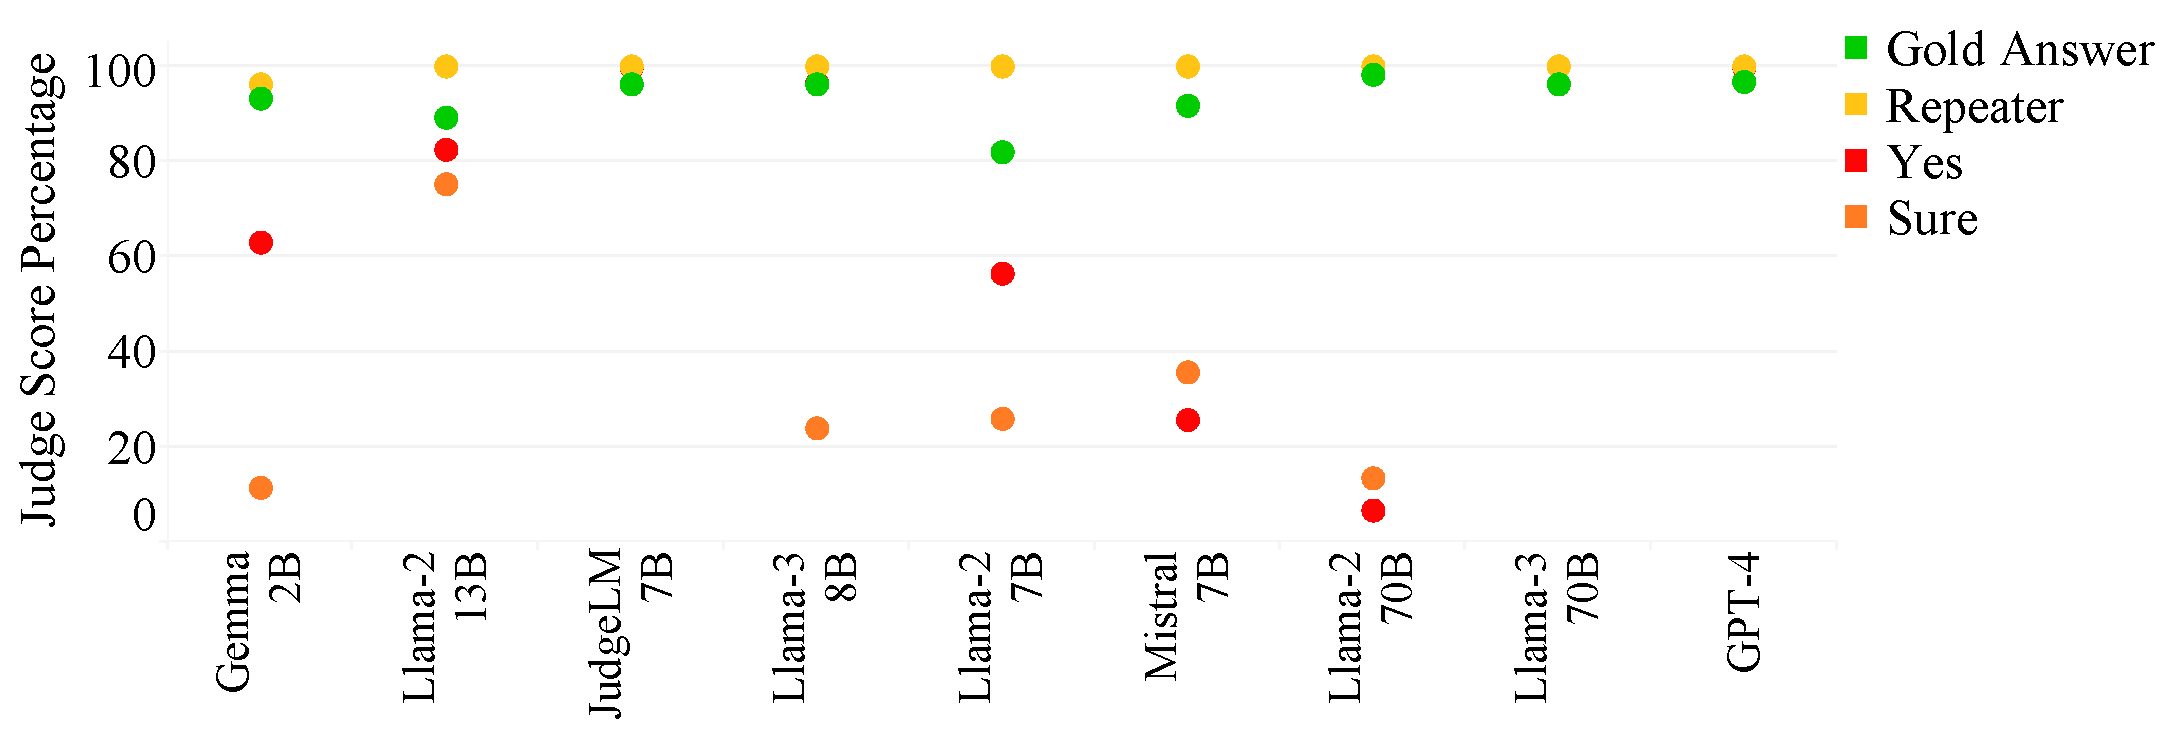
\includegraphics[width=0.825\textwidth]{figures/ConstantV2.pdf}
    \caption{\textbf{Judge responses to dummy answers.} 
    We investigate how \judgemodels respond to dummy answers.
    % , that either repeat the question, simply say `yes' or `sure' or verbatim match one of the reference answers. 
    \judgemodels remain robust when \evaluatormodels produce responses identical to the prompt (`repeater'), but are less robust when the responses are "Yes" and "Sure". Even when the answer matches one of the reference answers verbatim (`Gold answer'), judges do not always arrive at the correct judgement.
    }
    \label{fig:judge_dummy}
\end{figure*}

\subsection{\Judgemodel sensitivity to prompt length and specificity}
\label{sec:analysis:subsec:instructions}

Next, we investigate how prompt length and specificity affect \judgemodels' inferences to determine whether their performance is influenced by \textit{specificity} of the prompt. We use four prompt versions with varying length and specificity.

The first two prompts (\texttt{Without;guidelines;V1/V2}, 45 and 58 tokens) ask for an evaluation without further details. The longer prompts (\texttt{Guidelines;without;examples} and \texttt{Guidelines;with;examples}, 245 and 301 tokens) provide more elaborate guidance and examples. All prompts are listed in \cref{app:TMI}.

\cref{fig:TooMuchInfo} shows that \judge{\gpt}, \judge{Llama-3;70B}, and \judge{Llama-3.1;70B} exhibit low variance in human agreement as prompt length and specificity increases. Top performers show high alignment with humans even with minimal instructions, while they slightly improve with more detailed prompts. In contrast, other models lose alignment with increased instructions, likely due to difficulty processing complex instructions.

In a follow-up experiment, we investigate the impact of reference order (see \cref{app:ref-bias-exp}). \cref{app:ReferenceBiasExample1} and \cref{app:RefernceBiasExample2} shows that larger models maintain consistent judgments regardless of reference order, while smaller models, except \judge{Mistral;7B}, are more sensitive to it.

% Next, we study the impact of the prompt on the predictions of the \judgemodels, to understand if the success of various \judgemodels is related to the \textit{length} of the prompt, and to study the degree to which the judgments of the \judgemodels change with the \textit{specificity} of the prompt.

% We use four different prompt versions, varying in length and specificity.

% The first two prompts (\texttt{Without\;guidelines\;V1/V2}, 45 and 58 tokens, respectively) simply ask to evaluate the responses, without any further information, while more elaborate guidance and examples are given in the longer prompts (\texttt{Guidelines\;without\;examples} and \texttt{Guidelines\;with\;examples}, 245 and 301 tokens, respectively). 
% All prompts are listed in \cref{app:TMI}. 

% \cref{fig:TooMuchInfo} shows that \judge{\gpt}, \judge{Llama-3\;70B} and \judge{Llama-3.1\;70B} exhibit relatively low variance in their agreement with humans as the level of information and the length of the prompt increases.
% For this task, top performers' (\judge{\gpt}, \judge{Llama-3\;70B} and \judge{Llama-3.1\;70B}) implicit definition of a correct judgment seems well aligned with the provided instructions and thus shows high alignment with humans even if no specific instructions are provided.

% It can also be observed that only top performers appears to benefit from the more detailed instructions, with a slight upward trend, whereas the other models get less aligned with more instructions. This might be due to the less powerful judges not being able to follow many instructions in the prompt at the same time.
% % 
% In a follow-up experiment, we further investigate the impact of the order of the reference answers (for details, we refer to \cref{app:ref-bias-exp}). 
% \cref{fig:consistency} illustrates that larger \judgemodels consistently maintain their judgments regardless of the reference order, whereas smaller models -- with the exception of \judge{Mistral\;7B} -- are more sensitive to the reference order given in the prompt.

\subsection{Evaluating controlled responses}
\label{sec:analysis:subsec:judge-ability}

We conduct simple tests on the \judgemodels by having them evaluate dummy benchmark responses. In the first test, the answer is a verbatim reference from the dataset (always correct). In the next three tests, the answers are incorrect. For the second and third tests, the dummy \evaluatormodel responds with \texttt{``Yes''}, and \texttt{``Sure''} respectively. In the fourth test, the evaluated answer is a repetition of the question.

% Next, we perform simple tests on the \judgemodels by asking them to evaluate a set of dummy benchmark responses. For the first test, the answer to be evaluated for each question is one of the references from the dataset, verbatim (the answer is thus always correct).
% For the next three tests, the answer is always incorrect.
% In the second and third tests, the dummy \evaluatormodel always responds with \texttt{``Yes''}, and \texttt{``Sure''} for the second and third tests, respectively.
% For the fourth test, the evaluated answer is a repetition of the question.

% the answer to be evaluated is always incorrect, with the dummy \evaluatormodel always responding with \texttt{``Yes''}, and \texttt{``Sure''} for the 2nd and the 3rd tests, respectively, and simply repeating the question for the fourth test.
%

In \cref{fig:judge_dummy}, we observe that while some \judgemodels correctly identify and mark answers as correct (first test) or incorrect (next three tests), others, like \judge{Llama-2;70B}, incorrect evaluate many dummy answers, despite showing high human alignment on benchmark evaluations (see \cref{fig:llmalignment_b}). We hypothesize that when the answers are plausible but incorrect, judges can correctly identify them as wrong by comparing them with the reference. However, when the answer is unrelated (e.g., \texttt{``Yes''}, and \texttt{``Sure''}), \judgemodels may mistakenly mark them as correct, though further research is needed to clarify this behavior.

% In \cref{fig:judge_dummy}, we can see that while some \judgemodels are able to identify and correctly mark the answers as correct (for the first test) or incorrect (for the next three tests), some judges, notably \judge{Llama-2\;70B}, incorrectly evaluate a significant number of dummy answers, even though they show a relatively high alignment with humans on the benchmark evaluations (see \cref{fig:llmalignment_b}).
% % 
% We hypothesise that when the answers are plausible but incorrect (e.g.\ if the question asks about the name of the author of a book, and the \evaluatormodel gives the name of the wrong author), most judges are able to identify them as being incorrect (by comparing it with the reference answer). 
% However, the judges might get confused about what they are supposed to evaluate if the answer is completely unrelated to the question (such as the words \texttt{``Yes''} and \texttt{``Sure''}). 
% It is possible that, in this situation, a \judgemodel tries to evaluate one of the reference answers, thus marking it as correct, though further research is required to identify the cause of this behavior.



% \begin{figure}[H]
%     \begin{minipage}[b]{0.49\textwidth}
%         \centering
%         \includegraphics[width=\textwidth]{figures/BasevsChat7b.png}
%         % \caption{Comparison Scores for Llama 7B Base and Llama 7B Chat}
%     \end{minipage}
%     \hfill
%     \begin{minipage}[b]{0.49\textwidth}
%         \centering
%         \includegraphics[width=\textwidth]{figures/BasevsChat70b.png}
%         % \caption{Comparison Scores for Llama 70B Base and Llama 70B Chat}
%     \end{minipage}
%     \caption{Comparison of Llama 7B and Llama 70B Models}
%     \label{fig:comparison}
% \end{figure}



% From these observations, we can draw the conclusions that

% 1) There is a knowledge gap between base and chat models which gets more prominent in bigger models. \\
% 2) The ideal LLM evaluator is more lenient than the smaller models and more stricter than GPT \\
% 3) Base models are subject to more relaxed judgement as compared to Chat models.

\subsection{Leniency bias in \judgemodels}
\label{sec:leniency-bias}

% \begin{table}[t]
%     \centering
%     \begin{tabular}{lrrr}
    
%       \toprule
%       Evaluator & $\kappa$ & $P_e$ & $P_+$ \\
%       \midrule
%       Gemma 2B & 0.50 & 0.62 & 0.80 \\
%       Llama-2 7B & 0.66 & 0.68 & 0.36 \\
%       Mistral 7B & 0.72 & 0.75 & 0.75 \\
%       Llama-2 13B & 0.68 & 0.76 & 0.45 \\
%       Llama-2 70B & 0.80 & 0.79 & 0.94 \\
%       Llama-3 8B & 0.81 & 0.80 & 0.84 \\
%       Llama-3 70B & 0.84 & 0.84 & 0.79 \\
%       GPT-4 Turbo & 0.85 & 0.85 & 0.66 \\
%       \bottomrule
% \end{tabular}
% \caption{Estimated values of $P_e$ and $P_+$ for different \judgemodels}
% \label{tab:leniency-bias}
% \end{table}

Lastly, to get a general sense of the inherent biases or misalignment in the evaluation criteria that might be present in the judge models, we estimate if they have a positive or negative bias in their judgment.
To do so, we assume that a judge assigns the correct judgment (i.e.\ same evaluation as the ground truth) with a probability of $P_c$ and assigns the rest of the samples to be \texttt{``correct''} with a probability $P_+$, which we call their \textit{leniency bias}.
% present a crude but simple hypothesis: for a given \judgemodel and a given benchmark, the proportion of times where the evaluation criteria of the \judgemodel align with the provided instructions is given by $P_e$. 
% In the cases where the \judgemodel is not able to correctly understand the task or is not capable enough to evaluate according to the given criteria, it randomly gives an evaluation of \texttt{true} with probability $P_+$, and an evaluation of \texttt{false} with the remaining probability of $1-P_+$, independently of the correctness of the answer.
We estimate the values of $P_c$ and $P_+$ from the benchmark results\footnote{
The theoretical derivation of the expressions for $P_c$ and $P_+$, as well as the empirical validation for their estimated values can be found in \cref{app:leniency-bias}.}
and show them in \cref{tab:p-vals-full}. 
We observe that $P_+$ for most models is significantly higher than $0.5$ (\cref{fig:k-p-corr}), indicating a tendency of the \judgemodels to evaluate responses as \texttt{``correct''} when their evaluation criteria are not completely aligned with the provided instructions. 

\section {Conclusion}\label{sec:conclusion}

In this work, we conduct an extensive study of LLMs as judges, comparing them to human judges and automated evaluation methods. By focusing on a clean evaluation scenario with high inter-human agreement, we identify potential issues with the LLM-as-a-judge paradigm, separate from task ambiguity.

We find that smaller, cost-efficient models, like \judge{Mistral;7B}, are less effective than larger models such as \judge{\gpt}, \judge{Llama-3.1;70B}, and \judge{Llama-3;70B}, which are better aligned but still fall short of human alignment. Even with high alignment, their scores can differ by up to 5 points from human scores, highlighting the need for caution when using judges in more complex scenarios. We also note that the commonly used metric of \textit{percent aligned} fails to differentiate between judges effectively. We suggest future work adopt the more robust \scottspi metric for better distinction.

Next, we note that high alignment scores are not always necessary to \textit{discriminate} between models. While \judge{\gpt} and \judge{Llama-3} have excellent alignment scores, simpler and more cost-efficient models, like \judge{contains}, perform similarly in ranking \evaluatormodels, despite lower alignment scores and score deviations. For studies focused on ranking models rather than estimating exact scores, these approaches can be as suitable as more expensive ones.

Lastly, we run experiments to assess judge models' sensitivity to prompts, precision, recall, error types, leniency, and vulnerability to dummy answers. We find that smaller models are more likely to judge positively when in doubt, that lower-alignment models lack precision, and that better models are more robust across different prompts but harder to "steer." Some \judgemodels are easily fooled by dummy answers like \texttt{''Yes''} and \texttt{''Sure''} and are better at detecting completely incorrect answers than partially incorrect ones.

Overall, this work contributes to LLM evaluation by assessing judges in a clearly defined framework. Our results highlight the potential of LLMs as judges but caution against blindly trusting their judgments, even when aligned with humans. We recommend computing both percent agreement and \scottspi, paired with qualitative analysis, to avoid bias. We discuss limitations in \cref{app:limitations} and plan to expand our work to more complex scenarios in the future.

%%%%%%%
% In this work, we provide an extensive study of the properties of LLMs as judges, comparing them with human judges as well as automated evaluation methods.
% By focusing on a clean evaluation scenario in which inter-human agreement is high, we examine the potential issues with the LLM-as-a-judge paradigm, separately from the ambiguity and subjectivity in the task itself.
% %
% We find that even in straightforward setups, smaller and more cost-efficient models are less effective judges compared to the best available LLMs, such as \judge{Mistral\;7B}.
% \judge{\gpt}, \judge{Llama-3.1\;70B} and \judge{Llama-3\; 70B}, instead, are much better aligned, though they are still quite far from the alignment that humans have among each other.
% In some cases, despite their high alignment, their scores deviate from human scores with up to 5 points.
% Given the relative simplicity of the scenarios in which we deployed the judges, urging caution in using judge for more complex scenarios.
% Importantly, we noted that such patterns are virtually undetectable using the commonly deployed metric of \textit{percent aligned}, which barely discrimates between the considered judges.
% We suggest that future work instead considers the more robust metric \scottspi, which allows to distinguish judges much better.

% Next, we note that to \textit{discriminate} between models, high alignment scores are not an absolute necessity.
% While \judge{\gpt} and \judge{Llama-3} both have excellent alignment scores, simpler and more cost-efficient and even the lexical matching method \judge{contains} perform on par when discriminating between the \evaluatormodels in terms of their \textit{ranking}, despite having much lower alignment scores and score deviations.
% If the purpose of a study is to determine which model is better and not to estimate their actual scores, such approaches may thus be as suitable as the more expensive ones.

% Lastly, we run a range of experiments to investigate judge models' sensitivity to prompts, their precision and recall, their error types, how lenient they are, and how much they can be fooled by dummy answers. 
% We find that LLMs tend to judge positively when in doubt, and this is more pronounced for small models than for larger ones; that judge models with lower alignment lack precision rather than recall, that better models are generally more robust across different prompts, but are difficult to `steer' in their judgments; that some \judgemodels can be easily fooled by dummy answers such as \texttt{`Yes'} and \texttt{`Sure'}; and that \judgemodels are better at detecting completely incorrect answers than partially incorrect ones.
 
% Overall, this work adds to the realm of LLM evaluation research by assessing judges within a clearly defined and objective framework. Our results highlight the utility of using some LLMs as judges but also urge caution in blindly trusting their judgments, even if they are found to be well-aligned with humans.
% For practitioners using LLMs as judges -- regardless of the setup -- we recommend not only computing percent agreement, but also \scottspi, and pairing these with a qualitative analysis to ensure that conclusions from \judgemodels are less susceptible to biases. We further elaborate on the limitations of our work in \cref{app:limitations}. In the future, we plan to expand our work to increasingly more complex scenarios with more open-ended answers and variability and more generally assess how consistent our findings are across dataset samples, benchmarks, and prompt templates.
%%%%%%%%%%%%%%%%%%%%%%%%%%%%%%%%%%%%%%%%%%%%

% Our emphasis is on evaluating the inherent abilities of \judgemodels rather than their proficiency in assessing other LLMs. Understanding how judge LLMs operate and perform in objective settings helps establish benchmarks for their reliability and fairness. This knowledge is crucial for ensuring that AI systems, including those used in legal and decision-making contexts, uphold principles of transparency, accountability, and fairness.

% We also find that Judge LLMs are highly sensitive to prompt variations, with performance declining with overly complex or ambiguous instructions. Furthermore, our comparison highlights the consistent underperformance of fine-tuned models compared to pre-trained ones in objective assessments. These findings underscore the need for refinement in automatic grading system and use of Judge LLMs.



% In conclusion, we report that evaluations from different judges align poorly with human judgement. Judge LLMs do not exhibit any signs of systematic biases that may help us make an argument to use them. We also 

% \kc{Basically summarize here what are the answers that we found for the research questions that we put forward in the Experiments section. All answers should directly follow form the results of the experiments we performed.}


% textbf{1)} How well do the evaluations from different judges align with human evaluations? \textbf{2)} How is a alignment of evaluations related to the alignment of the final scores given by the judges? \textbf{3)} How similar are the rankings of evaluation models generated by the judge models compared to the rankings by humans? \textbf{4)} How sensitive are the judge models to the specific prompt provided to them to give a judgement? \textbf{5)} What are the similarities and differences in the mistakes made by different judges?

% \subsection{Future Work}
% These baseline results are a lot different from the previous run I did, with the difference being a slight change in the template (delimiting the questions, answers and references with “```” ), and skipping high ref count questions (although I don’t think the second change would make a difference). So that shows that the exact template used can be a big factor in the evaluations, and even GPT-4 is susceptible to small changes in the template.

%\section{Limitations}\label{app:limitations}

In our work, we have evaluated how 11 different LLMs fare as judges in a scenario in which judgements should be relatively straight-forward, and human alignment is high.
As any study, our work has several limitations as well as directions that we did not explore but would have been interesting too.
In this section, we discuss both.

\paragraph{Simplicity of the task}
As mentioned in the introduction of our work, the scenario in which judges are used are typically much more complicated than the scenario that we focussed on.
Specifically, judges are most often deployed in preference rankings (where two model responses are compared) or to judge complex answers that are difficult to automatically parse.
In such tasks, human agreement is often low, making it challenging to judge the judges themselves.
In our work, we have deliberately chosen for a simple task, in which human alignment is high.
The main premise is, that if a judge does not perform well in this simple setup, caution is suggested also in more complex setups -- if someone cannot do multiplication, why would they be able to solve ordinary differential equations.
Given the poor understanding of which abilities of LLMs generalise in what dimensions, however, more studies are needed to understand how our results generalise to various other scenarios.

\paragraph{Human alignment}
In an earlier version of this paper, due to the high cost of human annotations, we opted to select a single model for human annotation as we iteratively modified the exam taker prompt, few-shot examples, and guidelines. 
We selected the \eval{Llama2 7B} for this purpose with a random sample of 600 questions.
As this is only a single model, it is possible that our human alignment scores are biased because of that.
After, we have therefore extended our results with another 600 human-annotated examples from \eval{Llama3.1 70B}.

% This choice was made to establish a lower bound on human alignment by utilizing one of the smallest base models available. 
For \eval{Llama2 7B} The average alignment among human evaluators had a \scottspi of $96.36\pm1.46$,%
and the average percent agreement was $98.33\%\pm0.76\%$.
For \eval{Llama3.1 70B}, we noted that the average alignment among human evaluators had \scottspi of $95.78\pm0.30$,\% and the average percent agreement was $98.72\%\pm0.10\%$.
Given the similarity of these two numbers, we believe that these 1200 samples provide an adequate estimate.
In the paper, we take the average.
% Larger models typically achieve higher Exact Match (EM) scores, which often results in a smaller sample size needed for human annotations.  
% Before finalizing this methodology, we experimented with different chat models and GPT-4 but did not observe any appreciable difference in human alignment

\paragraph{Size of the judged samples}
As each of the \nexamtakersword \evaluatormodels requires human annotations for each sample, we restricted our analysis to 400 samples in total.
This sample size also allowed us to conduct manual annotations and error analysis within 75 human hours/200 GPU hours (see \cref{app:experiment-costs}) and give reliable confidence intervals while also providing the flexibility to compare a range of models. 
We were not able to increase the size due to the cost, but a statistical analysis (details provided in \cref{app:downsamplingstddev}) illustrated that the variance because of this sample size was very low.

\paragraph{Selection of judges}
With our selection of judges, we have stuck to autoregressive judges that can be used off-the-shelve, as well as one LLM specifically trained to judge.
They are -- at the moment of writing -- the ones that are most commonly used as LLM-judges, and we have tried to be comprehensive across size and family.
Nevertheless, we acknowledge that there are other judges that we could have considered as well.
As including more judges in -- compared to including more \evaluatormodels -- relatively straightforward because it requires only computational power, no manual annotation, we hope that others may evaluate their newly proposed judges using our setup as well.

% Similarly, We focused on the TriviaQA \cite{joshi2017triviaqa} dataset exclusively due to its clear references and structured questions, which ensured high inter-human annotator agreement. 
% In contrast, our experiments with other QA datasets like Natural Questions \cite{kwiatkowski2019natural} often faced challenges with question ambiguity, resulting in lower agreement among human annotators. 
% By choosing TriviaQA, we aimed to establish strong baselines with straightforward guidelines, allowing for consistent evaluations across different models without the confounding factor of ambiguous questions.
% In reporting our primary findings, we acknowledge in methodology (\cref{sec:methodology}) that the prompt template used in \cref{app:judge-prompt-template} is not as detailed as the human guidelines outlined in \cref{app:human_annotation_guidelines}. To address this, we conducted a parallel experiment using the human annotation guidelines in \judgemodels prompts. Our hope was to improve the judges' ability to assess underspecified or overspecified answers and responses with excessive verbosity. With human guidelines, we noticed that the "Contains" lexical match performed better. However, smaller models like Gemma 2B \citep{gemma2024gemma} and Judge LM 7B \citep{zhu2023judgelm} showed poor alignment with human annotators, achieving less than 20\%. This result supports our earlier concerns mentioned in \cref{sec:analysis:subsec:instructions}, where we pointed out that smaller models have difficulty following complex and nuanced instructions.

% From \cref{fig:llmalignment_w_human_guidelines}, it is evident that although this approach enhances the performance of the "Contains" judge, smaller models experience significant degradation. This finding aligns with our concerns noted in \cref{sec:analysis:subsec:instructions}, where we highlighted that smaller models struggle to follow complex and nuanced instructions.

% \centering
% \begin{figure}[h!]
%     \centering
% \includegraphics[width=0.7\textwidth, height=9cm]{figures/LLMAlignment_With_HumanGuidelines.pdf} 
%     \caption{ Kappa scores (red bars) and percent agreement (blue line) for difference judges when run with human guidelines. This setup skews judges like contains closer to human alignment but leads to worse alignment for EM (upto $\sim$ 30 points deviation from mean) and smaller judge models like Gemma 2B (1\%) \& JudgeLM-7B (18\%)}
%     \label{fig:llmalignment_w_human_guidelines}
% \end{figure}

\paragraph{Future work}
All in all, these differences underline how finicky using LLMs as judges can be, and with that confirm the overall conclusions of our study that much more work is needed to better understand the strengths and limitations of judge models across a wide range of scenarios and model accuracies.
We consider assessing the strengths across multiple different samples and tasks, which would require many more human annotations, outside the scope of this paper and leave such experimentation for future work.

% \section {Acknowledgements}
We would like to thank Mark Tygert for pointing us to the limitations of Cohen's Kappa and for helping us proofread \cref{app:cohenslimitation}.
AST, KC and VSR received assistance from GPU facilities provided by the University of Massachusetts, Amherst,  as well as GPT-4 funding was from the Center of Data Science at Manning College of Information and Computer Science, UMass Amherst.


\bibliography{bibliography}
% \bibliographystyle{acl_natbib}

\appendix
\newpage
\appendix
\renewcommand{\thesection}{\Alph{section}}

\section{Limitations}\label{app:limitations}

In our work, we have evaluated how 11 different LLMs fare as judges in a scenario in which judgements should be relatively straight-forward, and human alignment is high.
As any study, our work has several limitations as well as directions that we did not explore but would have been interesting too.
In this section, we discuss both.

\paragraph{Simplicity of the task}
As mentioned in the introduction of our work, the scenario in which judges are used are typically much more complicated than the scenario that we focussed on.
Specifically, judges are most often deployed in preference rankings (where two model responses are compared) or to judge complex answers that are difficult to automatically parse.
In such tasks, human agreement is often low, making it challenging to judge the judges themselves.
In our work, we have deliberately chosen for a simple task, in which human alignment is high.
The main premise is, that if a judge does not perform well in this simple setup, caution is suggested also in more complex setups -- if someone cannot do multiplication, why would they be able to solve ordinary differential equations.
Given the poor understanding of which abilities of LLMs generalise in what dimensions, however, more studies are needed to understand how our results generalise to various other scenarios.

\paragraph{Human alignment}
In an earlier version of this paper, due to the high cost of human annotations, we opted to select a single model for human annotation as we iteratively modified the exam taker prompt, few-shot examples, and guidelines. 
We selected the \eval{Llama2 7B} for this purpose with a random sample of 600 questions.
As this is only a single model, it is possible that our human alignment scores are biased because of that.
After, we have therefore extended our results with another 600 human-annotated examples from \eval{Llama3.1 70B}.

% This choice was made to establish a lower bound on human alignment by utilizing one of the smallest base models available. 
For \eval{Llama2 7B} The average alignment among human evaluators had a \scottspi of $96.36\pm1.46$,%
and the average percent agreement was $98.33\%\pm0.76\%$.
For \eval{Llama3.1 70B}, we noted that the average alignment among human evaluators had \scottspi of $95.78\pm0.30$,\% and the average percent agreement was $98.72\%\pm0.10\%$.
Given the similarity of these two numbers, we believe that these 1200 samples provide an adequate estimate.
In the paper, we take the average.
% Larger models typically achieve higher Exact Match (EM) scores, which often results in a smaller sample size needed for human annotations.  
% Before finalizing this methodology, we experimented with different chat models and GPT-4 but did not observe any appreciable difference in human alignment

\paragraph{Size of the judged samples}
As each of the \nexamtakersword \evaluatormodels requires human annotations for each sample, we restricted our analysis to 400 samples in total.
This sample size also allowed us to conduct manual annotations and error analysis within 75 human hours/200 GPU hours (see \cref{app:experiment-costs}) and give reliable confidence intervals while also providing the flexibility to compare a range of models. 
We were not able to increase the size due to the cost, but a statistical analysis (details provided in \cref{app:downsamplingstddev}) illustrated that the variance because of this sample size was very low.

\paragraph{Selection of judges}
With our selection of judges, we have stuck to autoregressive judges that can be used off-the-shelve, as well as one LLM specifically trained to judge.
They are -- at the moment of writing -- the ones that are most commonly used as LLM-judges, and we have tried to be comprehensive across size and family.
Nevertheless, we acknowledge that there are other judges that we could have considered as well.
As including more judges in -- compared to including more \evaluatormodels -- relatively straightforward because it requires only computational power, no manual annotation, we hope that others may evaluate their newly proposed judges using our setup as well.

% Similarly, We focused on the TriviaQA \cite{joshi2017triviaqa} dataset exclusively due to its clear references and structured questions, which ensured high inter-human annotator agreement. 
% In contrast, our experiments with other QA datasets like Natural Questions \cite{kwiatkowski2019natural} often faced challenges with question ambiguity, resulting in lower agreement among human annotators. 
% By choosing TriviaQA, we aimed to establish strong baselines with straightforward guidelines, allowing for consistent evaluations across different models without the confounding factor of ambiguous questions.
% In reporting our primary findings, we acknowledge in methodology (\cref{sec:methodology}) that the prompt template used in \cref{app:judge-prompt-template} is not as detailed as the human guidelines outlined in \cref{app:human_annotation_guidelines}. To address this, we conducted a parallel experiment using the human annotation guidelines in \judgemodels prompts. Our hope was to improve the judges' ability to assess underspecified or overspecified answers and responses with excessive verbosity. With human guidelines, we noticed that the "Contains" lexical match performed better. However, smaller models like Gemma 2B \citep{gemma2024gemma} and Judge LM 7B \citep{zhu2023judgelm} showed poor alignment with human annotators, achieving less than 20\%. This result supports our earlier concerns mentioned in \cref{sec:analysis:subsec:instructions}, where we pointed out that smaller models have difficulty following complex and nuanced instructions.

% From \cref{fig:llmalignment_w_human_guidelines}, it is evident that although this approach enhances the performance of the "Contains" judge, smaller models experience significant degradation. This finding aligns with our concerns noted in \cref{sec:analysis:subsec:instructions}, where we highlighted that smaller models struggle to follow complex and nuanced instructions.

% \centering
% \begin{figure}[h!]
%     \centering
% \includegraphics[width=0.7\textwidth, height=9cm]{figures/LLMAlignment_With_HumanGuidelines.pdf} 
%     \caption{ Kappa scores (red bars) and percent agreement (blue line) for difference judges when run with human guidelines. This setup skews judges like contains closer to human alignment but leads to worse alignment for EM (upto $\sim$ 30 points deviation from mean) and smaller judge models like Gemma 2B (1\%) \& JudgeLM-7B (18\%)}
%     \label{fig:llmalignment_w_human_guidelines}
% \end{figure}

\paragraph{Future work}
All in all, these differences underline how finicky using LLMs as judges can be, and with that confirm the overall conclusions of our study that much more work is needed to better understand the strengths and limitations of judge models across a wide range of scenarios and model accuracies.
We consider assessing the strengths across multiple different samples and tasks, which would require many more human annotations, outside the scope of this paper and leave such experimentation for future work.


\section{A brief explanation of the theoretical issues with Cohen's kappa}\label{app:cohenslimitation}

Cohen's Kappa Coefficient \citep{cohen1960kappa} is a statistic to measure inter-rater agreement for categorical responses.
Cohen's Kappa coefficient measures this agreement by computing the observed (percent) agreement between raters ($p_o$) and comparing it with the hypothetical probability of chance agreement ($p_e$), which is taken as a baseline, as follows:
\begin{equation}
\kappa \equiv \frac{p_o - p_e}{1 - p_e}
\end{equation}

In this equation, the chance agremeent $p_o$ constitutes the hypothetical probability that observed agreement occurred by chance, given the observed distributions of the considered raters, under the assumption that the probabilities the raters assign to the observed labels are independent.
Specifically, it is defined as:

\begin{equation*}
\begin{aligned}
p_e &= \sum_k \widehat{p_{k12}} =^{ind} \sum_k \widehat{p_{k1}} \widehat{p_{k2}} \\
    &= \sum_k \frac{n_{k1}}{N} \cdot \frac{n_{k2}}{N}
     = \frac{1}{N^2} \sum_k n_{k1} n_{k2}
\end{aligned}
\end{equation*}

where $\widehat{p_{k12}}$ is the estimated probability that rater 1 and rater 2 will classify the same item as $k$, rewritten to $\widehat{p_{k1}}\widehat{p_{k2}}$ under the assumption that $p_{k1}$ and $p_{k2}$ are independent.
The crux of the issue with this method of computation, is that $\widehat{p_{k1}}$ and $\widehat{p_{k2}}$ are estimated independently from the data.
As such, the chance agreement adjusts for the observed average differences between raters, which is in fact part of what we intend to measure.

To address this issue, Scott's Pi \citep{scott1995scottspi} instead defines the chance baseline under the assumption that the raters have the same distribution, which is estimated considering the joint distribution of rater 1 and rater 2, rather than considering them separately.
It defines $p_e$ as:

\begin{equation}
p_e = \sum_k \widehat{p_k^2} = \sum_k \sum_k (\frac{n_{k1} + n_{k2}}{2N})^2
\end{equation}

As such, contrary to Cohen's Kappa, it captures differences surpassing the chance agreement if rater 1 and rater 2 were in fact equivalent.
In other words, we compare against a baseline in which raters would be equivalent, and we measure how much they deviate from that.

Note that if the empirical distributions of rater 1 and rater 2 are the same, so will the values of Scott's Pi and Cohen's Kappa be.
This also implies that for larger observed (percent) alignment values, the values for Cohen's Kappa and Scott's Pi will be closer.



\section{Model and dataset details}\label{app:asset-details}

In \cref{tab:assets}, we show the different models and datasets used in our experiments, along with version and license details.


\begin{table*}[h]
    \centering
    \begin{tabular}{lll}
        \toprule
        Asset & Version & License \\
        \midrule
        TriviaQA & \href{https://huggingface.co/datasets/mandarjoshi/trivia_qa}{\texttt{mandarjoshi/trivia\_qa}} & apache-2.0 \\
        Llama-2 7B Base & \href{https://huggingface.co/meta-llama/Llama-2-7b-hf}{\texttt{meta-llama/Llama-2-7b-hf}} & llama2 \\
        Llama-2 7B Chat & \href{https://huggingface.co/meta-llama/Llama-2-7b-chat-hf}{\texttt{meta-llama/Llama-2-7b-chat-hf}} & llama2 \\
        Llama-2 13B Base & \href{https://huggingface.co/meta-llama/Llama-2-13b-hf}{\texttt{meta-llama/Llama-2-13b-hf}} & llama2 \\
        Llama-2 13B Chat & \href{https://huggingface.co/meta-llama/Llama-2-13b-chat-hf}{\texttt{meta-llama/Llama-2-13b-chat-hf}} & llama2 \\
        Llama-2 70B Base & \href{https://huggingface.co/meta-llama/Llama-2-70b-hf}{\texttt{meta-llama/Llama-2-70b-hf}} & llama2 \\
        Llama-2 70B Chat & \href{https://huggingface.co/meta-llama/Llama-2-70b-chat-hf}{\texttt{meta-llama/Llama-2-70b-chat-hf}} & llama2 \\
        Mistral 7B Base & \href{https://huggingface.co/mistralai/Mistral-7B-v0.1}{\texttt{mistralai/Mistral-7B-v0.1}} & apache-2.0 \\
        Mistral 7B Chat & \href{https://huggingface.co/mistralai/Mistral-7B-Instruct-v0.2}{\texttt{mistralai/Mistral-7B-Instruct-v0.2}} & apache-2.0 \\
        Llama-3 8B Chat & \href{https://huggingface.co/meta-llama/Meta-Llama-3-8B-Instruct}{\texttt{meta-llama/Meta-Llama-3-8B-Instruct}} & llama3 \\
        Llama-3 70B Chat & \href{https://huggingface.co/meta-llama/Meta-Llama-3-70B-Instruct}{\texttt{meta-llama/Meta-Llama-3-70B-Instruct}} & llama3 \\
        Llama-3.1 8B Chat & \href{https://huggingface.co/meta-llama/Meta-Llama-3.1-8B-Instruct}{\texttt{meta-llama/Meta-Llama-3.1-8B-Instruct}} & llama3.1 \\
        Llama-3.1 70B Chat & \href{https://huggingface.co/meta-llama/Meta-Llama-3.1-70B-Instruct}{\texttt{meta-llama/Meta-Llama-3.1-70B-Instruct}} & llama3.1 \\
        JudgeLM & \href{https://huggingface.co/BAAI/JudgeLM-7B-v1.0}{\texttt{BAAI/JudgeLM-7B-v1.0}} & Non-commercial license \\
        GPT-4 Turbo & \href{https://platform.openai.com/docs/models/gpt-4-turbo-and-gpt-4}{\texttt{gpt-4-turbo-2024-04-09}} & N/A \\
        % Qwen 0.5B Chat & \href{https://huggingface.co/Qwen/Qwen1.5-0.5B-Chat}{\texttt{Qwen/Qwen1.5-0.5B-Chat}} & tongyi-qianwen \\
        % Qwen 1.8B Chat & \href{https://huggingface.co/Qwen/Qwen1.5-1.8B-Chat}{\texttt{Qwen/Qwen1.5-1.8B-Chat}} & tongyi-qianwen \\
        % Qwen 4B Chat & \href{https://huggingface.co/Qwen/Qwen1.5-4B-Chat}{\texttt{Qwen/Qwen1.5-4B-Chat}} & tongyi-qianwen \\
        % Qwen 7B Chat & \href{https://huggingface.co/Qwen/Qwen1.5-7B-Chat}{\texttt{Qwen/Qwen1.5-7B-Chat}} & tongyi-qianwen \\
        % Qwen 14B Chat & \href{https://huggingface.co/Qwen/Qwen1.5-14B-Chat}{\texttt{Qwen/Qwen1.5-14B-Chat}} & tongyi-qianwen \\
        % Qwen 72B Chat & \href{https://huggingface.co/Qwen/Qwen1.5-72B-Chat}{\texttt{Qwen/Qwen1.5-72B-Chat}} & tongyi-qianwen \\
        \bottomrule
    \end{tabular}
\label{tab:assets}
        \captionsetup{skip=8pt} % Adjust space between table and caption
\caption{Version and license details for the different models and datasets used in experiments.}
\end{table*}


\section{Model evaluation prompt templates}\label{app:prompt-templates}

In \cref{app:template_pretrained} and \cref{app:template_finetuned}, we show the prompt templates used for the base and chat \evaluatormodels during the question answering process.

% \clearpage

\begin{figure*}[htbp]
    \centering
    \centering
    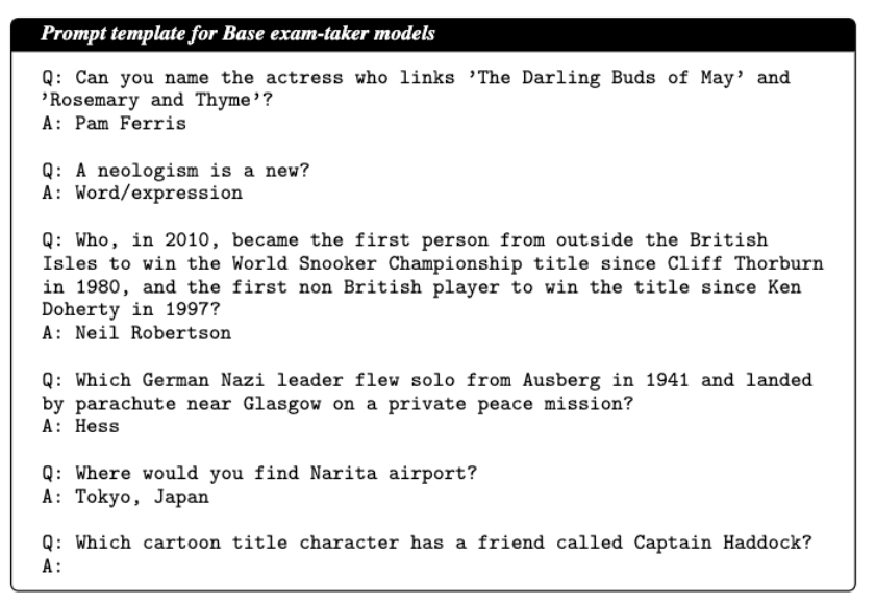
\includegraphics[width=0.8\linewidth]{figures/BaseExamTakerTemplate.pdf}
    \caption{Prompt template for base \evaluatormodels}
    \label{app:template_pretrained}
\end{figure*}

\begin{figure*}[htbp]
    \centering
    \centering
    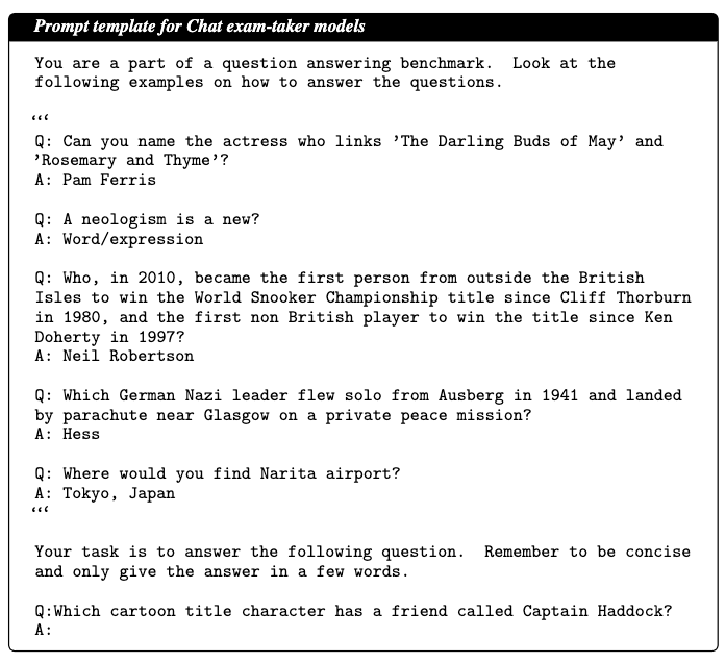
\includegraphics[width=0.8\linewidth, height=0.5\textheight]{figures/ChatExamTakerTemplate.pdf}
    \caption{Prompt template for Chat \evaluatormodels}
    \label{app:template_finetuned}
\end{figure*}


\section{Judge LLM Prompt templates}\label{app:judge-prompt-template}
In \cref{app:WithoutGuidelines}, we show the prompt template used to guide the \judgemodels during the evaluation process of a 400-question sample from the TriviaQA unfiltered dataset.

\begin{figure*}[h]
    \centering
        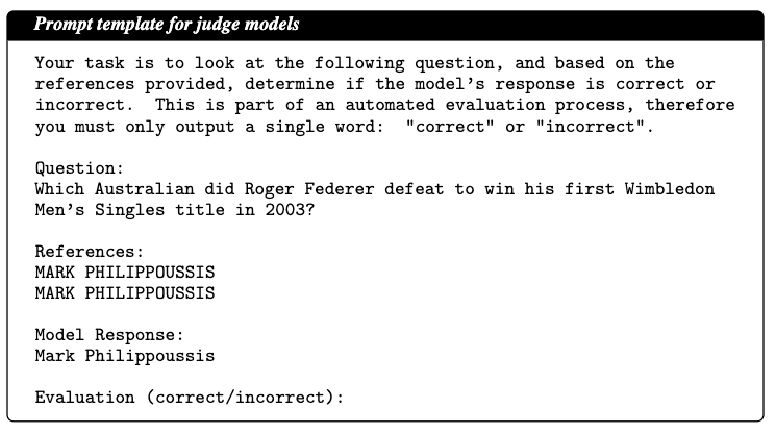
\includegraphics[width=0.8\textwidth, ]{figures/JudgePromptTemplate.pdf}
    \caption{Prompt templates for the \judgemodels}
    \label{app:WithoutGuidelines}
\end{figure*}

\section{Metrics for \judgemodels}
\label{app:metrics}

If one of the annotators is taken to be the reference, then the annotations of the other annotator can be categorized as true positives, false positives, true negatives, and false negatives, with the total number of each of them in a benchmark being represented by $T_P, F_P, T_N,$ and $F_N$ respectively.

\textbf{Percent agreement} is simply the ratio of the numbers of times two annotators agree with each other relative to the total number of annotations. This ratio can have values between $0$ and $1$. For the binary case, the alignment ratio $\rho$ 
%\kc{what symbol to use?} 
is given as

\begin{equation}
    \rho = \frac{T_P + T_N}{T_P + F_P + T_N + F_N}.
\end{equation}

\textbf{Scott's Pi}, \citep{scott1995scottspi}, measures the alignment of two annotators while also taking into account the possibility of agreement by pure chance. This coefficient usually has values above $0$ in most real-world situations. The value of Scott's Pi is given below where $p_o$ is the relative observed agreement, and $p_e$ is the hypothetical probability of chance agreement. 

\begin{figure*}[t]
\begin{equation*}
\pi = \frac{p_o - p_e}{1 - p_e} \nonumber \\
    = \frac{
        \left(\frac{TP + TN}{TP + TN + FP + FN}\right) - 
        \left(\frac{(TP + FP)(TP + FN) + (TN + FN)(TN + FP)}
        {(TP + TN + FP + FN)^2}\right)
    }{
        1 - 
        \left(\frac{(TP + FP)(TP + FN) + (TN + FN)(TN + FP)}
        {(TP + TN + FP + FN)^2}\right)
    }
\end{equation*}
\vspace{-1em}
\label{app:scott-pi}
\end{figure*}

\clearpage
\onecolumn
\section{Human Annotation Guidelines}
\label{app:human_annotation_guidelines}

\mytcolorbox{Human annotation guidelines}{You will be given a question, a set of reference answers and the answer given by an LLM. Your task is to judge if the answer given by the LLM is correct, as if you were the LLMs teacher grading their exam. An answer should be counted as correct if it is semantically equivalent to (one of the) reference answers. In doing so, please follow the following guidelines:}{\begin{itemize}
    \item Underspecified answers (e.g. "December" instead of "December 20") should be marked \textit{incorrect}.
    \item Answers that have more information than requested (e.g. "December 20, in Paris" instead of "December 20") should be marked correct, provided the extra information is not incorrect or contrasting the rest of the answer.
    \item Answers with unnecessary verbosity but correct answers should be marked correct (E.g. ``Thanks for asking this question! The correct answer is: ...").
\end{itemize}
If you have trouble judging whether the answer is correct, for instance because you feel you are lacking knowledge required to judge so, please indicate so by marking the answer "maybe correct" or ``maybe incorrect", so that we can further review it.}

\twocolumn
Preliminary research involved iterative refinement of human annotation guidelines to ensure consistency and reproducibility across annotators with general English semantic knowledge. CS graduate students served as annotators for this experiment. We provide the guidelines used for human evaluation below.

\section{Experiment costs}\label{app:experiment-costs}

The costs for the different experiments described in this work belong in three categories -- GPU-hours for running open-source models on one or more \texttt{Nvidia A100} GPUs, OpenAI credits for making API calls to OpenAI models,\footnote{Pricing details for OpenAI models are available at \url{https://openai.com/api/pricing/}} and human hours for manual annotations of benchmark responses. 
The estimated costs for the final reported experiments are given in \cref{tab:experiment-costs}. 
In addition to this, previous unreported experiments and trials had an approximate cost of 120 GPU-hours, 100 USD in OpenAI credits, and 50 human hours, bringing the total experimental cost for this work to approximately 200 GPU-hours, USD 125 OpenAI credits, and 75 human annotation hours.

\section{Statistical reliability of Evaluation sample} \label{app:downsamplingstddev}

Due to computational constraints discussed in \cref{app:limitations} and \cref{app:experiment-costs}, we limit our evaluation set to randomly sampled 400 questions from TriviaQA \citep{joshi2017triviaqa}. In this section, we further take 5 samples of 300 randomly selected questions from the evaluation set and calculate the mean and standard deviation of Scott's Pi. From \cref{tab:downsampletab}, it can be observed that even on down-sampled sets, the \scottspi values are similar to \cref{fig:llmalignment_b}. Standard deviation of all the \judgemodels from the mean \scottspi is also minimal, barring \judge{EM} lexical match.  

\begin{table}[H]
    \begin{tabular}{lcc}
        \toprule
        Judge Model & Mean \scottspi & Std Dev \\
        \midrule
        Llama3-70B & 0.88 & 0.0046 \\
        Llama3.1-70B & 0.88 & 0.0039 \\
        Llama3.1-8B & 0.78 & 0.0050 \\
        Llama2-13B & 0.75 & 0.0043 \\
        Llama2-70B & 0.69 & 0.0114 \\
        Mistral-7B & 0.67 & 0.0108 \\
        JudgeLM-7B & 0.66 & 0.0026 \\
        Contains & 0.64 & 0.0087 \\
        Llama3-8B & 0.60 & 0.0126 \\
        Llama2-7B & 0.47 & 0.0112 \\
        EM & 0.47  & 0.29 \\
        Gemma-2B & 0.26 & 0.007 \\
        \bottomrule
    \end{tabular}
     \label{tab:downsampletab}
    \centering \captionsetup{skip=8pt} % Adjust space between table and caption
     \caption{Weak \scottspi variation for the 5 down-sampled sets indicating robustness for the evaluation sample}
\end{table}

\section{Judge Scores}
\label{app:all_scores}

We show the scores assigned by each \judgemodel to each \evaluatormodel, visualised in \cref{fig:llmalignment_a} in \cref{tab:eval-scores}.



% \section{Too Much Info Confuses the LLM}
% \label{app:TMI}
% \textcolor{red}{v1 and v2}
% Here are the prompt templates used for this experiment. The simplest prompt used is \textit{Without Guidelines v1} (see \cref{app:WithoutGuidelines_v1}) where we define a sequential and structured process for the \judgemodel. In \textit{Without Guidelines v2} (see \cref{app:WithoutGuidelines_v2}), we add an additional focus on the overall task and outcome as well. 

% For \textit{Guidelines without examples} (see \cref{app:GuidelinesWithoutExamples}), we provide the \judgemodels with detailed instructions about the task at hand, along with explicit guidelines on how to evaluate the answers. Additionally, for \textit{Guidelines with examples}(see \cref{app:GuidelinesWithExamples}), we also provide examples to the \judgemodels for further reference.

\section{\Evaluatormodel base vs chat analysis}
\label{app:BaseVsChatSupp}

Given the human judgments we have available, we take the opportunity to investigate the performance differences between base and their corresponding chat models.
In \cref{tab:ScoresBaseChat}, we show the scores assigned by various \judgemodels to four base-chat pairs.
According to the default metric \judge{EM}, the base models outperform the chat models by a large margin.
Interestingly, while this difference gets smaller when the answers are judged by humans (second column) or \judge{GPT-4 Turbo}, there is still a substantial difference for all four pairs, suggesting that the difference is not merely an effect of the increased verbosity of the chat models.
Further evidence for that hypothesis is provided by \cref{fig:BaseChatPieChart}, in which we can see that while 14\% of the errors are shared between the base-chat pairs, almost another 14\% of the examples get judged correctly by the base models but not by the chat models, while the opposite happens in only 2.5\% of the cases.

\onecolumn
\begin{table}[H]
    \centering
    \begin{tabular}{lccc}
        \toprule
        Experiment & GPU-hours & OpenAI credits & Human hours \\
        \midrule
        Main benchmarks & 5 & 2 & - \\
        Main evaluations & 30 & 8 & 10 \\
        Human alignment & 2 & - & 9 \\
        Error analysis & 1.5 & - & 5 \\
        Controlled responses & 15 & - & - \\
        Leniency bias & 5 & 5 & - \\
        Guideline bias & 10 & 5 & 1 \\
        Reference bias & 5 & 4 & 1 \\
        \midrule
        \textbf{Total} & \textbf{73.5} & \textbf{24} & \textbf{26} \\
        \bottomrule
    \end{tabular}
    \label{tab:experiment-costs}
         \captionsetup{skip=8pt} % Adjust space between table and caption
     \caption{Estimated costs for the final reported experiments. GPU-hours are in equivalent \texttt{Nvidia A100} hours, OpenAI credits are in USD, and human hours are time spent in manual annotation.}
\end{table}

\begin{table}[h]
\label{tab:eval-scores}
\centering
    % \begin{tabular}{cccc@{\extracolsep{2mm}}ccc@{\extracolsep{2mm}}ccc@{\extracolsep{2mm}}c}
    \setlength{\tabcolsep}{5pt}
    \begin{tabular}{ccccccccccc}
    % \toprule
% \small
    &  \multicolumn{9}{c}{\textbf{Exam taker models}} \\
    \cmidrule{2-10}
    & \multicolumn{6}{c}{Llama2} & \multicolumn{2}{c}{Mistral} & GPT-4 \\ 
    & \multicolumn{3}{c}{Base} & \multicolumn{3}{c}{Chat} & Base & Instruct \\
% \begin{longtable}{|p{1.4cm}|p{1.1cm}|p{1.1cm}|p{1.1cm}|p{1.1cm}|p{1.1cm}|p{1.1cm}|p{1.1cm}|p{1.1cm}|p{1.1cm}|p{1.1cm}|}
% \hline
% \multicolumn{2}{|c|}{\multirow{2}{*}{}} & \multicolumn{9}{|c|}{\textbf{Exam Taker Models}} \\ \cline{3-11}
% \multicolumn{2}{|c|}{\multirow{2}{*}{}} & \multicolumn{6}{c|}{Llama 2} & \multicolumn{2}{c|}{Mistral} & \multicolumn{1}{c|}{} \\ \cline{3-11}
% \multicolumn{2}{|c|}{} & \multicolumn{3}{c|}{Base} & \multicolumn{3}{c|}{Chat} & \multicolumn{1}{c|}{Base} & \multicolumn{1}{c|}{Instruct} &  \\ \hline
\textbf{Judge Models} & 7B  & 13B & 70B & 7B & 13B & 70B & \multicolumn{2}{c}{7B} \\
\cmidrule[1pt]{2-10}
Llama 3.1 8B & 65.25 & 75.00 & 83.50 & 60.25 & 70.50 & 75.50 & 73.75 & 59.00 & \textbf{89.00} \\ 
Llama 3.1 70B & 62.00 & 74.25 & 85.00 & 55.50 & 64.75 & 74.00 & 72.25 & 60.50 & \textbf{92.25} \\ \midrule
Llama 3 8B & 76.00 & 83.25 & 91.50 & 73.25 & 82.75 & 85.25 & 81.75 & 76.0 & \textbf{97.25} \\ 
Llama 3 70B & 64.25 & 75.50 & 86.50 & 57.00 & 64.00 & 75.75 & 73.5 & 62.50 & \textbf{92.75} \\ \midrule
Llama 2 7B & 80.50 & 85.25 & 92.00 & 80.50 & 70.75 & 90.75 & 84.00 & 83.25 & \textbf{97.75} \\ 
Llama 2 13B & 68.25 & 75.50 & 86.50 & 63.25 & 62.75 & 77.50 & 74.50 & 67.50 & \textbf{93.5} \\ 
Llama 2 70B & 71.25 & 80.5 & 90.25 & 67.50 & 74.75 & 81.25 & 80.0 & 72.5 & \textbf{96.75} \\ \midrule
Mistral 7B & 72.50 & 80.75 & 90.50 & 69.00 & 74.75 & 82.50 & 80.25 & 72.00 & \textbf{96.25} \\ \midrule
Gemma 2B & 79.75 & 87.00 & \textbf{91.25} & 58.50 & 41 & 68.50 & 84.0 & 55.75 & 80.50 \\ \midrule
JudgeLM & 69.50 & 77.75 & 86.25 & 63.75 & 48.0 & 82.75 & 77.25 & 71.0 & \textbf{94.50} \\ \midrule
GPT-4 & 60.50 & 71.50 & 82.50 & 54.50 & 59.0 & 73.0 & 69.75 & 56.50 & \textbf{90.0} \\ \midrule
Exact Match & 46.75 & 56.00 & \textbf{63.75} & 24.00 & 0.25 & 36.25 & 59.50 & 20.25 & 58.25 \\ 
Contains Match & 50.75 & 60.00 & 68.00 & 39.00 & 46.25 & 59.50 & 57.25 & 44.00 & \textbf{70.00} \\ \midrule
Human Eval & 62.50 & 72.75 & 83.75 & 56.00 & 56.50 & 72.25 & 71.75 & 60.75 & \textbf{91.50} \\
\bottomrule
\end{tabular}
 \captionsetup{skip=8pt} % Adjust space between table and caption
\caption{\Judgemodel score card for every \evaluatormodel.}
\end{table}

\twocolumn




% \begin{subfigure}[b]{0.6\textwidth}
% \renewcommand{\arraystretch}{0.7} % Reduce row spacing
% \setlength{\tabcolsep}{3pt} % Reduce column spacing
% \begin{tabular}{@{}lrrrrr@{}}
% \toprule
% \multicolumn{1}{c}{} & \multicolumn{5}{c}{\textbf{Judge models}} \\ \cmidrule(lr){2-6}
% \makecell{Base-Chat\\ pair} & EM & Human & \makecell{GPT-4\\Turbo} & \makecell{Llama-2\\70B} & \makecell{Llama-2\\7B} \\ \midrule
% \makecell{Llama-2\\7B} & 22.75 & 6.25 & 6.50 & 4.25 & 3.25 \\ \cmidrule(lr){1-6}
% \makecell{Mistral\\7B} & 39.25 & 11.00 & 19.75 & 2.75 & -11.75 \\ \cmidrule(lr){1-6}
% \makecell{Llama-2\\13B} & 55.25 & 16.25 & 17.50 & -3.75 & -6.00 \\ \cmidrule(lr){1-6}
% \makecell{Llama-2\\70B} & 27.50 & 11.50 & 13.00 & 4.25 & 22.25 \\ \bottomrule
% \end{tabular}
% \caption{}
% \label{tab:DeltaValuesBaseChat}
% \end{subfigure}

\begin{table}[b]
    \centering
\label{tab:ScoresBaseChat}
 \captionsetup{skip=8pt} % Adjust space between table and caption
\caption{Scores of base and chat models by various judges}
\setlength{\tabcolsep}{6pt}
\begin{tabular}{p{2.5cm}cccccccccc}
\toprule
& \multicolumn{10}{c}{\textbf{Judge models}} \\ \cmidrule(lr){2-11}
    \makecell{Base-Chat\\ pair} & \multicolumn{2}{c}{EM} & \multicolumn{2}{c}{Contains} & \multicolumn{2}{c}{Human} & \multicolumn{2}{c}{\makecell{GPT-4\\Turbo}} & \multicolumn{2}{c}{\makecell{Llama-3\\70B}} \\
    \cmidrule{2-11}
    & Base & Chat & Base & Chat & Base & Chat & Base & Chat & Base & Chat \\
    \makecell{Llama-2 7B} & \textbf{46.75} & 24.00 & \textbf{50.75} & 39.00 & \textbf{62.25} & 56.00 & \textbf{60.50} & 54.50 & \textbf{64.25} & 57.00\\
    \makecell{Mistral 7B} & \textbf{59.50} & 20.25 & \textbf{57.25} & 44.00 & \textbf{71.75} & 60.75 & \textbf{69.75} & 56.50 & \textbf{73.50} & 62.50\\
    \makecell{Llama-2 13B} & \textbf{ 56.00} & 0.25 & \textbf{60.00} & 46.25 & \textbf{72.75} & 56.50 & \textbf{75.00} & 59.00 & \textbf{76.50} & 64.00\\
    \makecell{Llama-2 70B} & \textbf{63.75} & 36.25 &  \textbf{68.00} & 59.50 & \textbf{83.75} & 72.25 & \textbf{82.50} & 73.00 & \textbf{86.50} & 75.75\\
\bottomrule
\end{tabular}
\end{table}

We consider two alternative hypotheses:\begin{itemize}\setlength\itemsep{0.1em}
    \item[i)] The chat models have a worse understanding of the particular prompt format, which is tuned more to fit base models; or
    \item[ii)] The chat models have `unlearned' some knowledge during their alignment training.
\end{itemize}

To disentangle these two factors, we manually analyse 400 questions for \eval{Llama-2 70B} and \eval{Llama-2 70B-chat}, using our earlier error codes.
The results, shown in \cref{fig:comparisonBarplot}, sugest that, at least to some extent, the difference between base and chat models is in fact due to `unlearning' of knowledge: while the number of errors is more or less equal among most categories, there is a stark difference in the \emph{incorrect entity} category.
Substantially more often than the base models, the chat models do answer the question with a semantically plausible but incorrect entity.
In \cref{tab:KnowledgeUnlearningExample1}-\cref{tab:KnowledgeUnlearningExample3}, we provide examples of such cases.
The results do not show any evidence to support the first hypothesis: the number of errors where the answer cannot be parsed or is just entirely incorrect does not differ between base and chat models.

\section{\Evaluatormodel ranking correlation }
\label{app:correlationcoefftable}
% In \cref{tab:judges_rho_reversed}, we show the Spearman's rank correlation coefficient \citep{spearman1904spearman} ($\rho$) with human judgment. 
% Since $\rho$ > 0.7 is considered well aligned, only \judge{Llama-7B and \judge{Gemma-2B} have poor rank correlation with human judgment.} 


In \cref{tab:judges_rho_reversed}, We use the Spearman Rank correlation coefficient  \citep{spearman1904spearman} to assess the rankings of the \evaluatormodels. To validate these rankings, we randomly select 6 out of \nexamtakers \evaluatormodels across 5 samples, subsequently calculating the mean ($\rho$) and standard deviation ($\sigma$) of the rankings. The results reveal that the \judge{contains} model exhibits the highest stability and $\rho$ among the rankings, while the majority of judge models achieve a coefficient exceeding 0.7, indicating a strong alignment. Notably, smaller models such as \judge{Mistral 7B} perform on par with \judge{\gpt}, highlighting the robustness of smaller models in maintaining rankings.

\begin{table}[H]
\label{tab:judges_rho_reversed}
    \centering
    \begin{tabular}{lcc}
        \toprule
        Judges & $\rho$ & $\sigma$ \\
        \midrule
        Contains & 0.99 & 0.02 \\
        Mistral-7B & 0.98 & 0.03 \\
        GPT-4 & 0.98 & 0.03 \\
        Llama2-13B & 0.95 & 0.18 \\
        JudgeLM-7B & 0.95 & 0.05 \\
        Llama2-7B & 0.94 & 0.04 \\
        Llama3.1-70B & 0.94 & 0.07 \\
        Llama3-70B & 0.93 & 0.05 \\
        Llama3.1-8B & 0.89 & 0.10 \\
        Llama3-8B & 0.86 & 0.07 \\
        Llama2-70B & 0.84 & 0.13 \\
        Gemma-2B & 0.71 & 0.20 \\
        EM & 0.67 & 0.13 \\
        \bottomrule
    \end{tabular}
            \captionsetup{skip=5pt}
    \caption{Spearman Rank Correlation Coefficient $\rho$.}
\end{table}

% \clearpage
\section{Too much info confuses judges}
\label{app:TMI}
In \cref{app:WithoutGuidelines_v1}-\ref{app:GuidelinesWithExamples}, we report the guidelines we used for the experiments in \cref{sec:analysis:subsec:instructions}. 
The simplest prompt used is \textit{Without Guidelines v1} (see \cref{app:WithoutGuidelines_v1}) where we define a sequential and structured process for the \judgemodel. 
In \textit{Without Guidelines v2} (see \cref{app:WithoutGuidelines_v2}), we add an additional focus on the overall task and outcome as well. 
% 
For \textit{Guidelines without examples} (see \cref{app:GuidelinesWithoutExamples}), we provide the \judgemodels with detailed instructions about the task at hand, along with explicit guidelines on how to evaluate the answers. 
Additionally, for \textit{Guidelines with examples}(see \cref{app:GuidelinesWithExamples}), we also provide examples to the \judgemodels for further reference.


% \begin{itemize}[noitemsep]
% \item Knowledge unlearning by the chat models or Loss in knowledge (Correct Answer by Base model and Wrong Answer by Chat model) - $\mathcal{L}_{knowledge}$
% \item Error in judgment by \judgemodels (Right answer by Chat model but wrong judgment or Wrong answer by Base model but judged as right) - $\epsilon$
% \item Misc (Chat model fails to understand the prompt or answer Cut off) - $\mu$
% \end{itemize}

% \[
% \begin{array}{cc}
% \Delta_{\text{Human}} = \mathcal{L}_{knowledge} + \mu & \hspace{2cm} \Delta_{\text{LLM}} = \mathcal{L}_{knowledge} + \mu \pm \epsilon
% \end{array}
% \]

%%%%%%%%%%%%%%%%%%%%%%%%%
% Storyline
% 1) First we show the difference in scores and show not many 'Answer cut off' or other errors for chat models and hence its mostly Knowledge unlearning that contributes to delta in scores between Base and Chat models
% 2) Then we have to explain why is the delta varying across all judge models since Knowledge unlearning is same no matter what judge model we use. So here we say that its upto the judge model. Bigger judge = lineant scoring, smaller judge = harsher. Hence decrease in delta. Additionally, Knowledge unlearning is greater in bigger Base-Chat pairs
%%%%%%%%%%%%%%%%%%%%%%%%%%

% Assuming there is zero error in human judgment, $\epsilon$ in $\Delta_{\text{Human}}$ = 0. 

% The plots in \cref{fig:BaseChatPieChart} and \cref{fig:comparisonBarplot} suggest knowledge unlearning, as the Chat model provides more incorrect answers than the Base model, with the majority of these errors classified as 'incorrect entities' or 'under specification' (examples in \cref{app:BaseVsChatSupp}). 
% Specifically, \cref{fig:comparisonBarplot} shows that the \eval{Llama2 70B} Chat model answers a higher number of questions as 'incorrect entity' compared to the corresponding base model. 
% Furthermore, the Chat model provides too few entities in more responses than the Base model, indicating knowledge unlearning due to its inability to provide all the required entities for correct answers.
\onecolumn
\begin{figure}[t]
\centering
\begin{subfigure}{0.6\textwidth}
    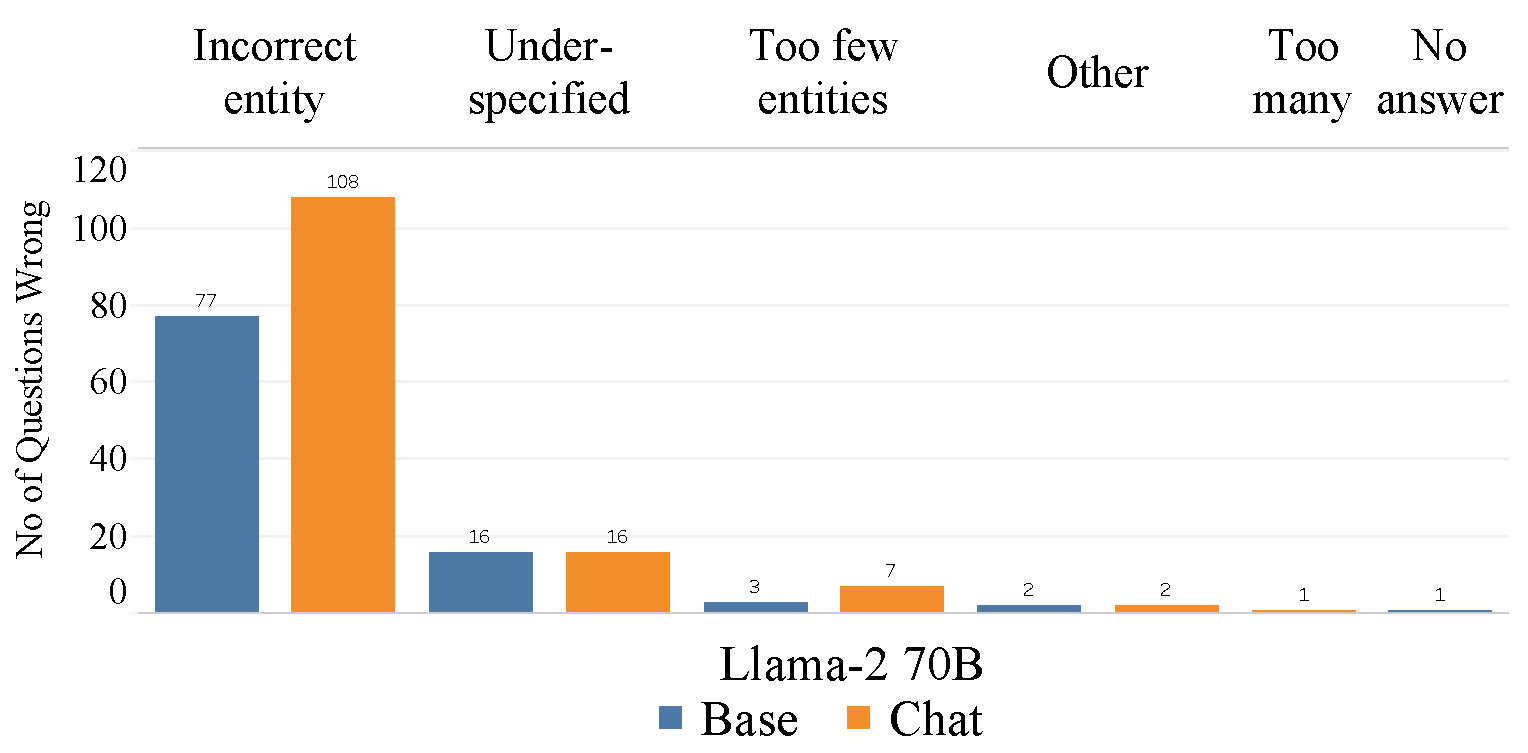
\includegraphics[width=\textwidth]{figures/ErrorCode.pdf}
    \caption{}
     \label{fig:comparisonBarplot}
\end{subfigure}
%
\hfill
%
\begin{subfigure}{0.39\textwidth}
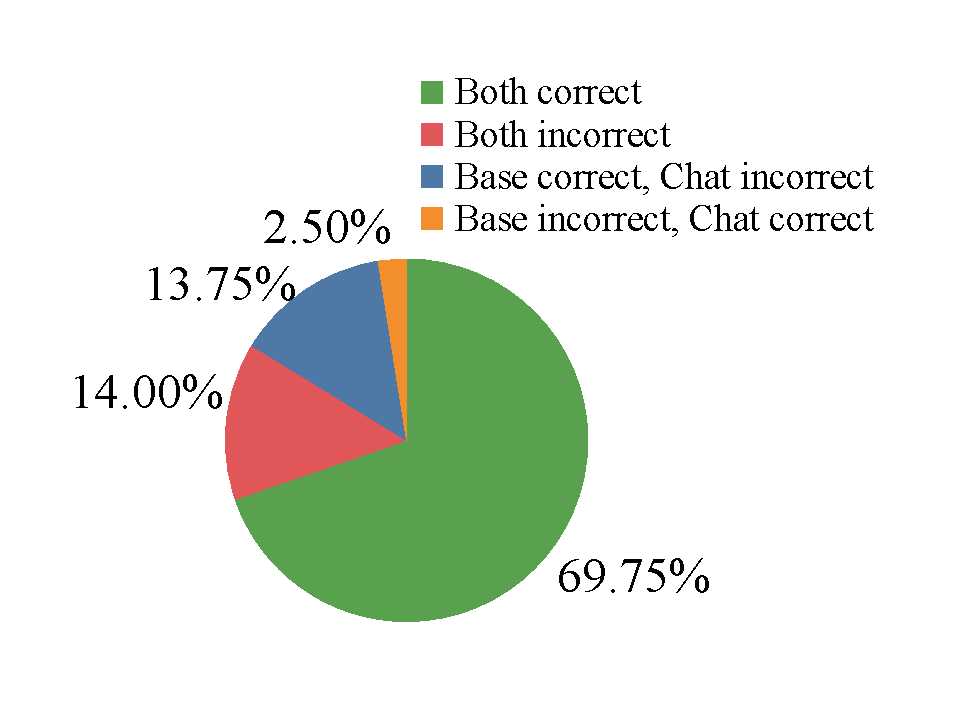
\includegraphics[width=\textwidth]{figures/PieChart.pdf}
% \vspace{15pt}
\caption{}
\label{fig:BaseChatPieChart}
\end{subfigure}
\caption{a) Distribution of incorrect question counts by error codes for \eval{Llama2 70B} Base vs Chat \evaluatormodels evaluated on 400 questions. b) Pie chart showing the percentage of questions categorized by the judgment from Base and Chat models.}
\end{figure}



% Additionally, \cref{fig:BasevsChat} shows with an increase in model size, \judge{GPT-4 Turbo} as a judge has a similar Kappa and alignment score with humans only for the Chat models. This implies that while bigger \judgemodels effectively parse and evaluate the verbose responses from the chat models, the main problem lies in the accuracy of their answers, which leads to a lower judge score and further suggesting knowledge unlearning.

% Furthermore, \cref{fig:BasevsChat} demonstrates that although the Llama-2 Base models have higher judge scores compared to the Chat models, the $\kappa$ score and percent agreement of \judge{GPT} increase for the Chat models and decrease for the Base models as the model size grows. 
% This indicates that the issue with the Chat models lies in the accuracy of their answers, resulting in lower judge scores, rather than an error in parsing their verbose responses. 
% This further suggests the unlearning of knowledge by the Chat models.

% Interestingly, across all \judgemodels, as the size of the \evaluatormodel increases, $\Delta$ also increases, suggesting that $\mathcal{L}_{knowledge}$ between the Base and Chat models widens as the model size grows. % \dieuwke{This doesn't seem to be true to me from the numbers: Llama 2 70B has a smaller difference than Llama-2 13B.

%Moreover, as the \judgemodel size gets smaller, the $\Delta_{\text{LLM}}$ values decreases, well beyond the observed $\Delta_{\text{Human}}$. 
% Given that $\mathcal{L}_{knowledge}$ and $\mu$ remain constant across all the \judgemodels, the only variable changing here is $\pm \epsilon$. 

% The scores from \cref{tab:eval-scores} indicate that the base \evaluatormodels are evaluated more strictly, while the chat \evaluatormodels are evaluated too leniently by the smaller \judgemodels. 
% This results in $\Delta_{\text{LLM}}$s that are smaller and sometimes negative, in contrast to the absolute scores that deviate significantly from the true scores. 
% One possible explanation is that the smaller \judgemodels are tricked by the verbose responses of the Chat \evaluatormodels into rewarding them with higher scores. However, this does not hold true for the larger \judgemodels.

% \begin{figure}[H]
% \centering
%     \centering
%     \includegraphics[width=\textwidth]{figures/BasevsChat.pdf}
%     \caption{Evaluation Metrics for LLama2 Base and Chat \evaluatormodel pairs evaluated by \judge{GPT-4 Turbo}}
%     \label{fig:BasevsChat}
% \end{figure}
\definecolor{darkgreen}{rgb}{0.0, 0.5, 0.0}
\begin{table}[H]
\centering
\label{tab:KnowledgeUnlearningExample1}
\begin{tabular}{|>{\raggedright\arraybackslash}m{2.5cm}|>{\raggedright\arraybackslash}m{10cm}|}
\hline
\multicolumn{2}{|c|}{\textbf{Question:}} \\
\multicolumn{2}{|c|}{\texttt{Which British artist's works include `The First Real Target'?}} \\
\hline
\textbf{References} & \rule{0pt}{3ex}\texttt{Peter Blake, Peter Balke, Sir Peter Blake}\rule[-1ex]{0pt}{1ex} \\
\hline
\textbf{LLama-2 70B Base} & \rule{0pt}{3ex}\textcolor{darkgreen}{\texttt{Peter Blake}}\rule[-1ex]{0pt}{1ex} \\
\hline
\textbf{LLama-2 70B Chat} & \rule{0pt}{3ex}\textcolor{red}{\texttt{Patrick Caulfield}}\rule[-1ex]{0pt}{1ex} \\
\hline
\textbf{Mistral 7B Base} & \rule{0pt}{3ex}\textcolor{red}{\texttt{David Hockney}}\rule[-1ex]{0pt}{1ex} \\
\hline
\textbf{Mistral 7B Chat} & \rule{0pt}{3ex}\textcolor{red}{\texttt{Damien Hirst}}\rule[-1ex]{0pt}{1ex} \\
\hline
\end{tabular}
\label{tab:KnowledgeUnlearningExample1}
\captionsetup{skip=5pt}
\caption{Knowledge unlearning example 1.}
\end{table}

\begin{table}[H]
\label{tab:KnowledgeUnlearningExample2}
\centering
\begin{tabular}{|>{\raggedright\arraybackslash}m{2.5cm}|>{\raggedright\arraybackslash}m{10cm}|}
\hline
\multicolumn{2}{|c|}{\textbf{Question:}} \\
\multicolumn{2}{|c|}{\texttt{Who was the first cricketer to score 10,000 test runs?}} \\
\hline
\textbf{References} & \rule{0pt}{3ex}\texttt{Sunil Gavaskar, Sunil Manohar Gavaskar, SM Gavaskar, Sunny gavaskar, Gavaskar}\rule[-1ex]{0pt}{1ex} \\
\hline
\textbf{LLama-2 70B Base} & \rule{0pt}{3ex}\textcolor{darkgreen}{\texttt{Sunil Gavaskar}}\rule[-1ex]{0pt}{1ex} \\
\hline
\textbf{LLama-2 70B Chat} & \rule{0pt}{3ex}\textcolor{red}{\texttt{Sachin Tendulkar}}\rule[-1ex]{0pt}{1ex} \\
\hline
\textbf{Mistral 7B Base} & \rule{0pt}{3ex}\textcolor{red}{\texttt{Sachin Tendulkar}}\rule[-1ex]{0pt}{1ex} \\
\hline
\textbf{Mistral 7B Chat} & \rule{0pt}{3ex}\textcolor{red}{\texttt{Sachin Tendulkar}} \texttt{was the first cricketer to score 10,000 runs in Test matches.}\rule[-1ex]{0pt}{1ex} \\
\hline
\end{tabular}
\label{tab:KnowledgeUnlearningExample2}
\captionsetup{skip=5pt}
\caption{Knowledge unlearning example 2}
\end{table}


\begin{table}[H]
\label{tab:KnowledgeUnlearningExample3}
\centering
\begin{tabular}{|>{\raggedright\arraybackslash}p{2.5cm}|>{\raggedright\arraybackslash}p{10cm}|}
\hline
\multicolumn{2}{|c|}{\textbf{Question:}} \\
\multicolumn{2}{|c|}{\parbox{12cm}{\texttt{`Uncle Harry's Coat' was the first garment produced by which famous jacket manufacturer, based in Simonside, Newcastle Upon Tyne?}}} \\
\hline
\textbf{References} & \rule{0pt}{3ex}\texttt{Barbour}\rule[-1ex]{0pt}{1ex} \\
\hline
\textbf{LLama-2 70B Base} & \rule{0pt}{3ex}\textcolor{darkgreen}{\texttt{Barbour}}\rule[-1ex]{0pt}{1ex} \\
\hline
\textbf{LLama-2 70B Chat} & \rule{0pt}{3ex}\textcolor{darkgreen}{\texttt{Barbour}}\rule[-1ex]{0pt}{1ex} \\
\hline
\textbf{Mistral 7B Base} & \rule{0pt}{3ex}\textcolor{darkgreen}{\texttt{Barbour}}\rule[-1ex]{0pt}{1ex} \\
\hline
\textbf{Mistral 7B Chat} & \rule{0pt}{3ex}\textcolor{red}{\texttt{Jack Walker \& Sons}}\rule[-1ex]{0pt}{1ex} \\
\hline
\end{tabular}
\label{tab:KnowledgeUnlearningExample3}
\captionsetup{skip=5pt}
\caption{Knowledge unlearning example 3}
\end{table}

\clearpage

\begin{figure}[H]
    \centering
    \resizebox{0.8\textwidth}{!}{
        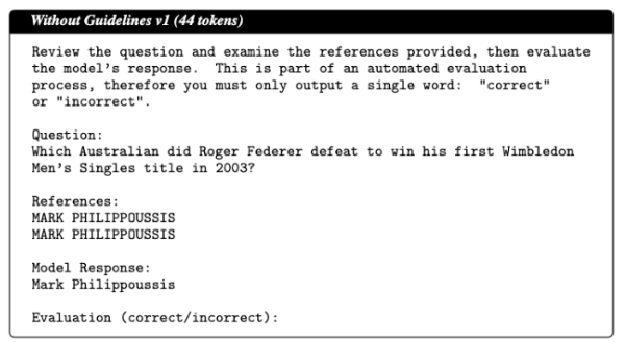
\includegraphics{figures/WithoutGuidelinesv1.pdf}
    }
    \caption{\textit{Without Guidelines v1} prompt template for the \judgemodels}
    \label{app:WithoutGuidelines_v1}
\end{figure}

\begin{figure}[t]
    \centering
    \resizebox{0.8\textwidth}{!}{
        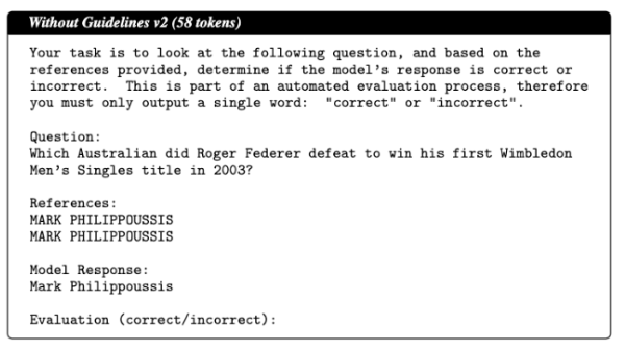
\includegraphics{figures/WithoutGuidelinesv2.pdf}
    }
    \caption{\textit{Without Guidelines v2} prompt template for the \judgemodels}
    \label{app:WithoutGuidelines_v2}
\end{figure}

\begin{figure}[h]
    \centering
    \resizebox{0.7\textwidth}{!}{
        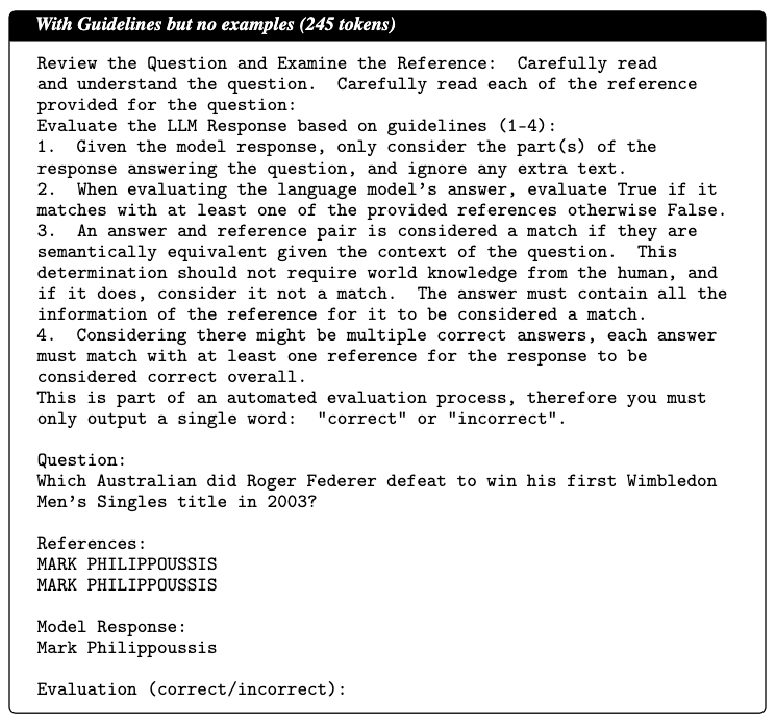
\includegraphics{figures/WithGuidelinesNoExamples.pdf}
    }
    \caption{\textit{Guidelines without examples} Prompt template for the \judgemodels}
    \label{app:GuidelinesWithoutExamples}
\end{figure}

% \vspace{-0.75cm}

\begin{figure}[ht]
    \centering
    \resizebox{0.7\textwidth}{!}{
        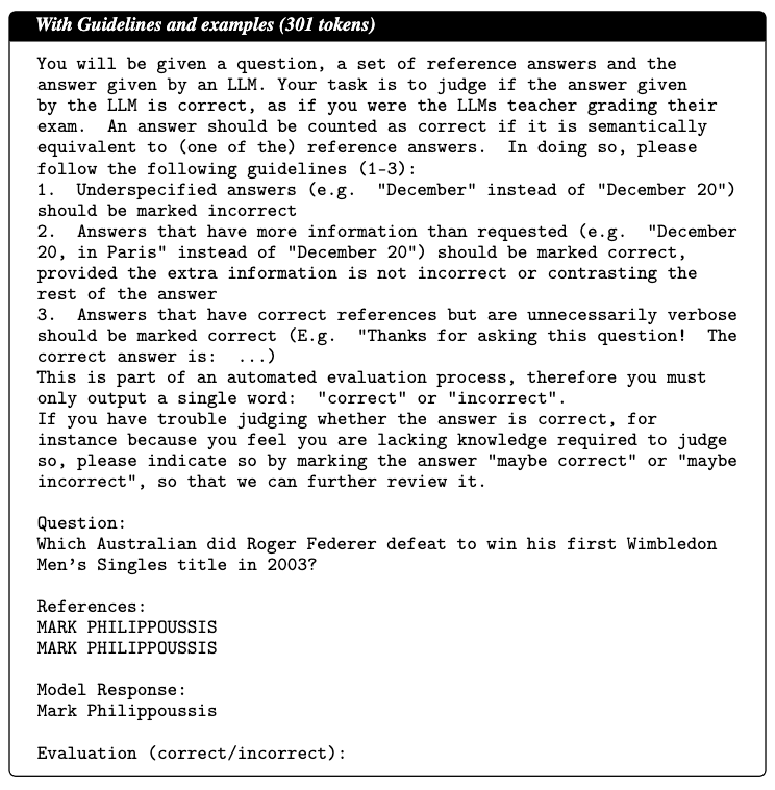
\includegraphics{figures/WithGuidelinesAndExamples.pdf}
    }
    \caption{\textit{Guidelines with Examples} Prompt template for the \judgemodels}
    \label{app:GuidelinesWithExamples}
\end{figure}

% \begin{table}[h]
%     \centering
%     \small
%     \setlength{\tabcolsep}{4pt} % Adjust column separation
%     \renewcommand{\arraystretch}{1.2} % Adjust row separation
%     \begin{tabular}{p{2.5cm}|p{1.0cm}|p{1.0cm}|p{1.0cm}|p{1.0cm}|p{1.0cm}}
%     \toprule
%     \makecell[l]{Prompt\\Template} & \makecell[l]{Llama-2\\7B} & \makecell[l]{Llama-2\\13B} & \makecell[l]{Llama-2\\70B} & \makecell[l]{Mistral\\7B} & \makecell[l]{GPT-4} \\
%     \midrule
%     \makecell[l]{Without \\ Guidelines v1 (44)} & 0.66 & 0.67 & \textbf{0.87} & 0.68 & 0.87 \\
%     \midrule
%     \makecell[l]{Without \\ Guidelines v2 (58)} & \textbf{0.67} & \textbf{0.73} & 0.82 & \textbf{0.75} & 0.89 \\
%     \midrule
%     \makecell[l]{Guidelines \\ w/o Examples (245)} & 0.43 & 0.42 & 0.73 & \textbf{0.75} & \textbf{0.93} \\
%     \midrule
%     \makecell[l]{Guidelines \\ with Examples (301)} & 0.39 & \textbf{0.73} & 0.70 & 0.61 & 0.90 \\
%     \bottomrule
%     \end{tabular}
%     \vspace{6pt} % Adjust the space here
%     \caption{Kappa scores with humans for various \judgemodels across different prompt templates.}
%     \label{tab:TMI_Kappa}
% \end{table}

\begin{figure}[htbp]
    \centering
    \resizebox{0.6\textwidth}{!}{
        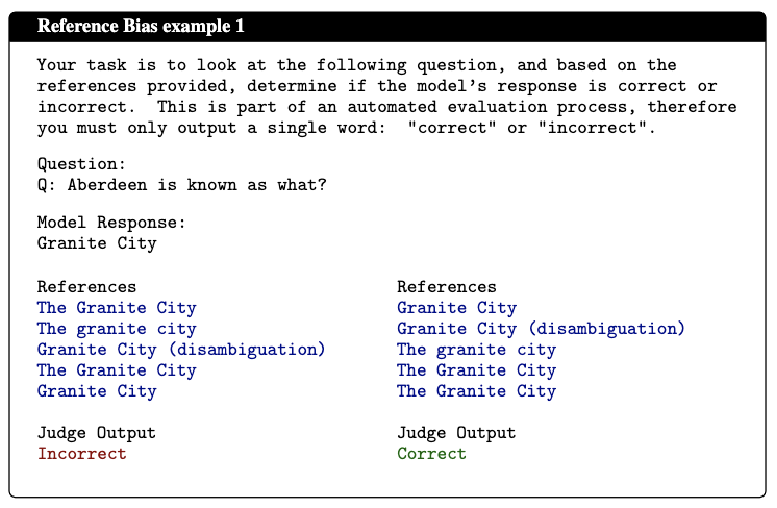
\includegraphics{figures/ReferenceBiasExample1.pdf}
    }
    \caption{Example of \judge{Llama2-7B} getting confused when the order of the references are changed}
    \label{app:ReferenceBiasExample1}
\end{figure}

\begin{figure}[H]
    \centering
    \resizebox{0.6\textwidth}{!}{
        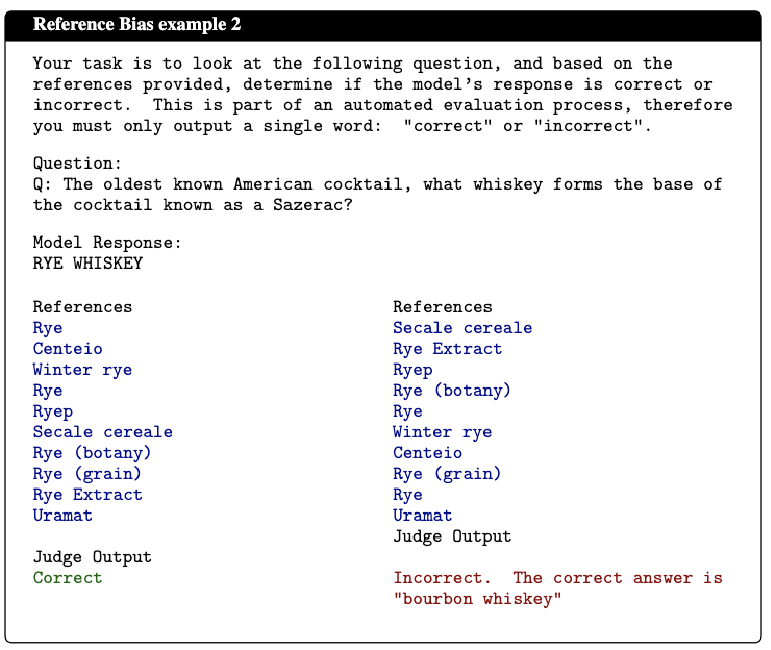
\includegraphics{figures/ReferenceBiasExample2.pdf}
    }
    \caption{Example of \judge{Llama2-7B} failing to identify the task by changing the order of the references.}
    \label{app:RefernceBiasExample2}
\end{figure}

\clearpage
\twocolumn
\section{\Judgemodels are sensitive to reference order}
\label{app:ref-bias-exp}

We investigate the judges' sensitivity to reference order by providing the same prompt, question and model response to the \judgemodels, but shuffling the reference order in three different permutations. We compute the consistency score of the model as the percentage of questions for which it gives the same judgment all the 3 times. 
%
% \dieuwke{Give formula of how we compute it.}
We observe that the model is more likely to evaluate an answer as correct if the corresponding reference appears early in the list of references (see \cref{app:ReferenceBiasExample1}).
% Additionally another factor that makes a judge LLM a good judge is consistency.
%
The smaller \judgemodels sometimes fail to capture all the information in the prompt, and provide judgement based on their own knowledge rather than going by the references (see  \cref{app:RefernceBiasExample2}).

% \begin{figure}[H]
%     \centering
%     \resizebox{0.9\textwidth}{!}{
%         \includegraphics{figures/Consistency_Plot.pdf}
%     }
%     \caption{Consistency Score and Average Kappa score with Humans for different \judgemodels for 3 random reference order permutation runs}
%     \label{app:GuidelinesWithExamples}
% \end{figure}
% \begin{table}[H]
% \centering
% \vspace{0.5em} % Adjust the spacing here
% \begin{tabular}{|c|c|c|c|c|c|c|c|c|}
% \hline
% & Exact-match & Llama2 7B & Llama2 13B & Llama2 70B & Mistral 7B & GPT 4T \\
% \hline
% Default & 42.00 & 49.50 & 52.50 & 62.00 & 61.50 & 57.25\\
% \hline
% Shuffled & 42.00 & 48.50 & 54.25 & 61.75 & 61.75 & 57.75\\
% \hline
% \end{tabular}
% \vspace{1em} % Adjust the spacing between caption and table
% \caption{judgment Scores for different ordering of the references given during judging for Llama-7B Base as the Exam-taker model}\label{table:reference_consistency}
% \end{table}


\section{Leniency Bias}\label{app:leniency-bias}

As described in \cref{sec:leniency-bias}, for the purpose of the leniency bias experiments, we assume that a judge assigns the correct judgment with a probability of $P_c$ and randomly assigns the rest of the samples to be \texttt{“correct”} with a probability $P_+$.
%
In this section, we derive the mathematical expressions for $P_c$ and $P_+$. We assume that in the case of misalignment between the evaluation criteria of guidelines and \judgemodels, the probability of getting an evaluation of \texttt{``correct''} is independent of the actual correctness of the answer (i.e.\ the \judgemodel effectively flips a coin to give out its judgement). For any given benchmark and \judgemodel, we denote the ground-truth score as $s$, and the true positive and true negative rates as $t_P$ and $t_N$, respectively, all normalized to be between $0$ and $1$.

Now, based on our assumptions, the true positives, where the \evaluatormodel response is correct, and also correctly identified by the \judgemodel to be correct, would be comprised of two possible cases: 1) The judge evaluates it correctly according to the given evaluation criteria with a probability of $P_c$; and 2) The judge does not evaluate it according to the given criteria with a probability of $1-P_c$, but the evaluation still happens to be correct with a probability of $P_+$. With the total ratio of the correct responses being $s$, the true positive rate is therefore given by --

\begin{equation}\label{eq:tp}
    t_P = s[P_c + (1-P_c)P_+]
\end{equation}

Similarly, the true negatives, where the \evaluatormodel response is incorrect, and also correctly identified by the \judgemodel to be incorrect, would also be comprised of two cases: \textbf{1)} The judge evaluates it correctly according to the given evaluation criteria with a probability of $P_c$.\textbf{2)} The judge does not evaluate it according to the given criteria with a probability of $1-P_c$, but the evaluation still happens to be correct with a probability of $1-P_+$. With the total ratio of the incorrect responses being $1-s$, the true negative rate is therefore given by --

\begin{equation}\label{eq:tn}
    t_N = (1-s)[P_c + (1-P_c)(1-P_+)].
\end{equation}

Using \cref{eq:tn}, we can derive the following. 

\begin{align}
    t_N &= (1-s)[P_c + (1-P_c)(1-P_+)] \\
    &= P_c + 1 - P_+ - P_c + P_cP_+ \\
    &\quad - sP_c  -s + sP_+ + sP_c - sP_cP_+ \\
    &=  1 - P_+ + P_cP_+ -s + sP_+  - sP_cP_+ \\
    &= 1 - s - P_+(1 - P_c - s + sP_c) \\
    &= 1 - s - P_+(1-s)(1-P_c) \\
    \implies P_+ &=\frac{1-s - t_N}{(1-s)(1-P_c)} \\
    &= \frac{1 - \frac{t_N}{1-s}}{1-P_c}
\end{align}

Substituting the value of $P_+$ in \cref{eq:tp}, we get:

\begin{align}
    t_P &= s[P_c + (1-P_c)P_+] \\
    &= s\Bigg[P_c + (1-P_c)\frac{1 - \frac{t_N}{1-s}}{1-P_c}\Bigg] \\
    &= s\bigg[P_c + 1 - \frac{t_N}{1-s}\bigg] \\
    \implies \frac{t_P}{s} &= P_c + 1 - \frac{t_N}{1-s} \\
    \implies P_c &= \frac{t_P}{s} + \frac{t_N}{1-s} - 1
\end{align}

The values of $P_c$ and $P_+$ can be estimated from observed data using the derived expressions. 
% In this experiment, we include Qwen models \citep{qwen} of varying sizes, in our judge ensemble to increase the number of data points for this study.
The estimated probabilities using this method, with human evaluation as the reference, are shown in \cref{tab:p-vals-full}.

To validate these derived values, we observe the correlation between the estimated values of $P_c$ and  Scott's Pi ($\pi$). 
As shown in \cref{fig:k-p-corr}, we observe that the estimated values of $P_c$ are highly correlated to the \scottspi values for the \judgemodels, with a Pearson correlation coefficient of $0.98$.

\begin{figure}[H]
\begin{subfigure}[b]{0.45\textwidth}
    \centering
    
    \begin{tabular}{lrrr}
      \toprule
      \Judgemodel & $\pi$ & $P_c$ & $P_+$ \\
      \midrule
          \judge{Gemma-2B} & 0.26 & 0.38 & 0.87 \\
          \judge{Llama2-7B} & 0.47 & 0.63 & 0.75 \\
          \judge{Llama3-8B} & 0.59 & 0.63 & 0.74 \\
          \judge{JudgeLM-7B} & 0.65 & 0.68 & 0.19 \\
          \judge{Mistral-7B} & 0.66 & 0.70 & 0.87 \\
          \judge{Llama2-70B} & 0.69 & 0.66 & 0.99 \\
          \judge{Llama2-13B} & 0.74 & 0.74 & 0.87 \\
          \judge{Llama3.1-8B} & 0.77 & 0.77 & 0.82 \\
           \judge{GPT-4} & 0.87 & 0.87 & 0.69 \\
          \judge{Llama3.1-70B} & 0.88 & 0.88 & 0.82 \\
          \judge{Llama3-70B} & 0.88 & 0.87 & 0.90 \\
      \bottomrule
\end{tabular}
\caption{}
\label{tab:p-vals-full}
\end{subfigure}%
%
\hspace{1cm}
%
\begin{subfigure}[t]{0.45\textwidth}
  \centering
  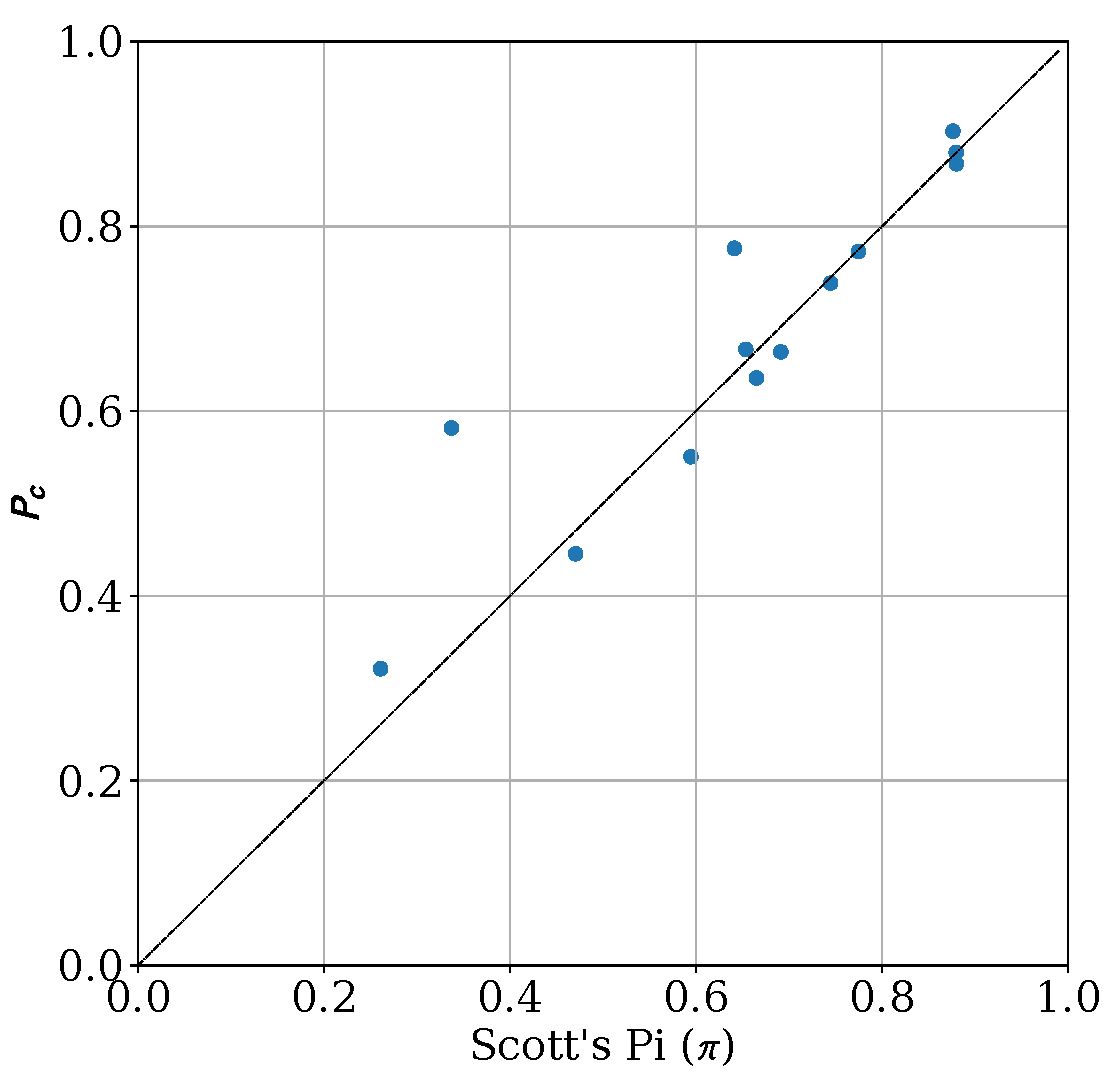
\includegraphics[width=\linewidth]{figures/corr9.pdf}
  \caption{}
  \label{fig:k-p-corr}
\end{subfigure}
\caption{a) Estimated values of $P_c$ and $P_+$ for different \judgemodels. b) Pearson's correlation coefficient between $\pi$ and $P_c$ for \judgemodels.}
\label{fig:leniency-bias-full}
\end{figure}

\begin{figure}[t]
    \centering
    \begin{subfigure}[b]{0.4\textwidth}
        \centering
        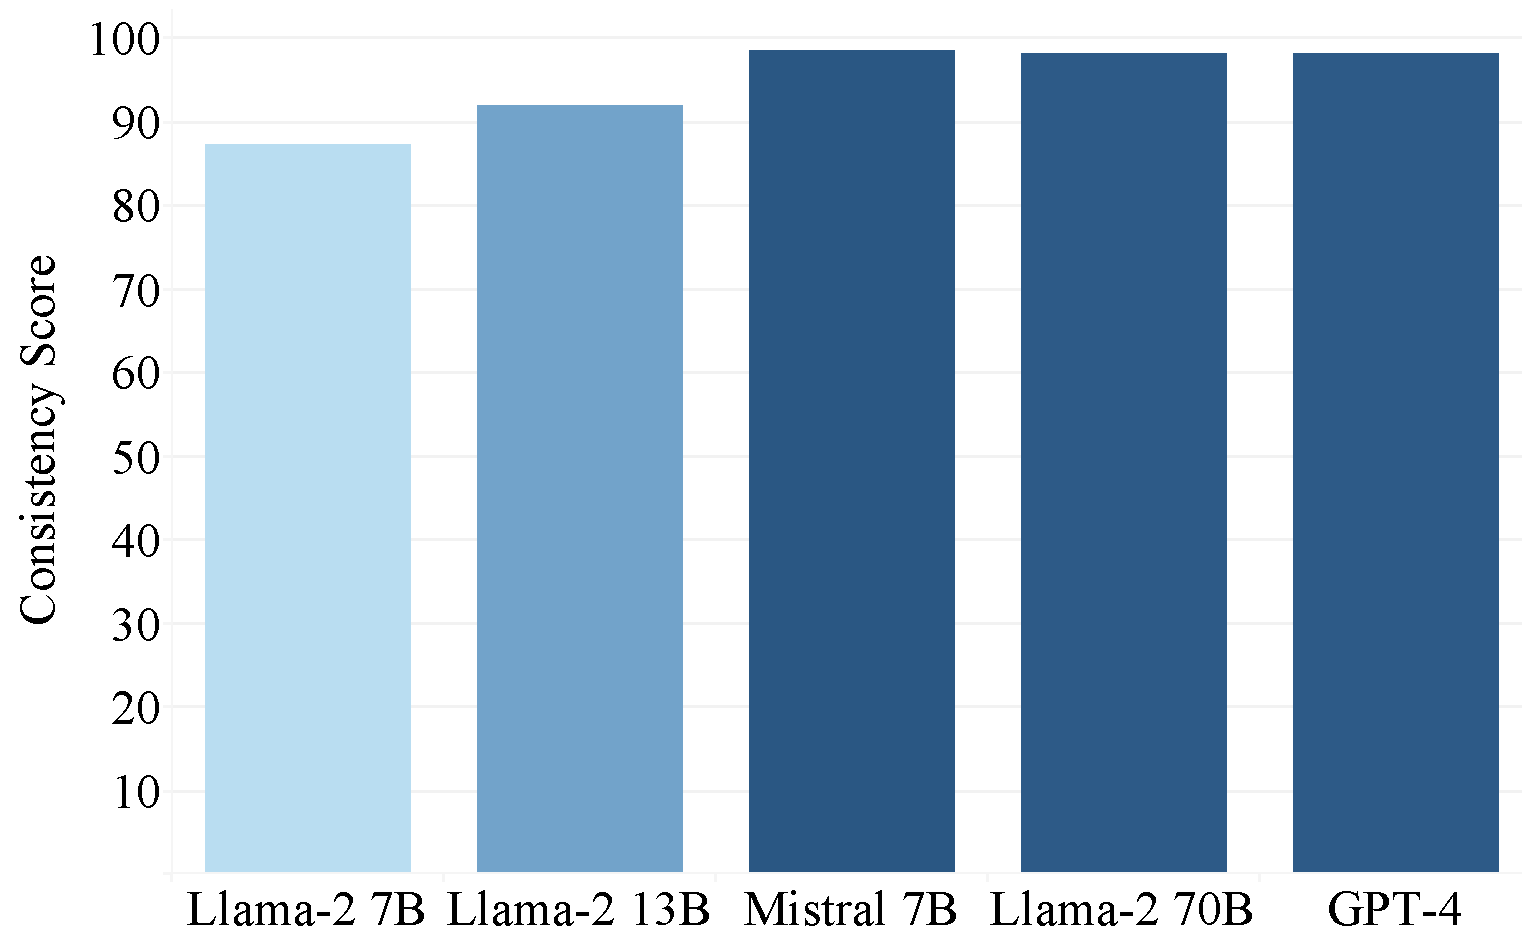
\includegraphics[width=\textwidth]{figures/Consistency.pdf}
        \label{fig:consistency}
    \end{subfigure}
    \caption{\textbf{Leniency bias and answer consistency.} Consistency score, defined as the percentage of questions for which the \judgemodel gives the same judgment for three different answer orders.}
\end{figure}

% \section{Evaluating base versus chat models} \label{sec:analysis:subsec:basevschat}

% \begin{table}[ht]
% \centering
% \vspace{0.5em} % Adjust the spacing here
% \begin{tabular}{ccccc}
% \multicolumn{1}{c}{\rule{0pt}{1em}} & \multicolumn{1}{c}{\rule{0pt}{1em}\judge{Human}} & \multicolumn{1}{c}{\rule{0pt}{1em}\judge{GPT}} & \multicolumn{1}{c}{\rule{0pt}{1em}\judge{Llama2-70B}} & \multicolumn{1}{c}{\rule{0pt}{1em}\judge{Llama2-7B}}\\ \hline
% \toprule\toprule
% Llama 7B & \rule{0pt}{1em}6.75 & \rule{0pt}{1em}9.5 & \rule{0pt}{1em}4.75 & \rule{0pt}{1em}1.75\\ 
% \midrule
% Mistral 7B & \rule{0pt}{1em}10.75 & \rule{0pt}{1em}11.5 & \rule{0pt}{1em}7.5  & \rule{0pt}{1em}6.25\\
% \midrule
% Llama 13B & \rule{0pt}{1em}16.5 & \rule{0pt}{1em}9 & \rule{0pt}{1em}3.75 & \rule{0pt}{1em}3.75\\
% \midrule
% Llama 70B & \rule{0pt}{1em}10 & \rule{0pt}{1em}10.25 & \rule{0pt}{1em}10  & \rule{0pt}{1em}7 \\
% \bottomrule
% \end{tabular}
% \vspace{1em} % Adjust the spacing between caption and table
% \caption{Difference in Evaluation Scores between different Base - Chat \evaluatormodel pairs for different \judgemodels}
% \label{tab:BasevsChat}
% \end{table} 


\end{document}
